\chapter{Geothermal Exploration Machine-Learning Results}\label{ch5:ml_results}

Chapter \ref{ch3:expl_ml_prep} outlined the machine-learning and uncertainty-analysis strategy for characterizing geothermal gradient, a proxy for the heat-risk element, across the Southwestern NM study area. This chapter reviews the results of applying that strategy with the curated data set described in Appendix \ref{app:A_data_layers}. In addition, this chapter places insights from the model results and uncertainty evaluation in context with mitigating risks associated with geothermal exploration.

\section{Logistic Regression} \label{ch5:lr_model}

\subsection{Hyperparameter Tuning} \label{ch5:lr_tuning}

\begin{wraptable}{R}{0.55\linewidth}
\centering
\begin{tabular}{c|c|c|c|}
\cline{2-4}
                                 & \textbf{WDS}   & \textbf{WDS4}  & \textbf{WDS8}  \\ \hline
\multicolumn{1}{|c|}{\bftt{C} % https://tex.stackexchange.com/questions/215482/how-do-i-get-texttt-with-bold-face-in-latex
}          & 0.170 & 0.085 & 0.085 \\ \hline
\multicolumn{1}{|c|}{\bftt{Accuracy$_{train}$}} & 0.703 & 0.701 & 0.709 \\ \hline
\multicolumn{1}{|c|}{\bftt{Accuracy$_{test}$}}  & 0.611 & 0.709 & 0.701 \\ \hline
\multicolumn{1}{|c|}{\bftt{AUC$_{train}$}} & 0.892 & 0.877 & 0.882 \\ \hline
\multicolumn{1}{|c|}{\bftt{AUC$_{test}$}}  & 0.785 & 0.891 & 0.875 \\ \hline
\end{tabular}
\singlespacing
\caption[Logistic regression hyperparameter tuning results]{Logistic regression hyperparameter tuning results for each data set. Accuracy and AUC model statistics are split into train (in-sample) and test (out-of-sample) values.}
\label{tab:logreg_tuning}
\end{wraptable}
The logistic regression (LR) model used in this analysis \citep{pedregosa_scikit-learn_2011} includes a single tunable hyperparameter, \verb|C|. Rather than rely on the pre-split training and validation subsets defined in Section \ref{ch3:strat_sample} to tune this hyperparameter, the subsets were re-combined and stratified-sampled as part of a 10-fold CV process. ROC AUC OvR was used as the scoring metric. Results vary for the different input data sets; CV results for WDS show a clear maximum AUC marking the optimal value for \verb|C|, whereas CV for WDS4 and WDS8 demonstrate a leveling-off trend, and the optimal value must be selected near the elbow (Figure \ref{fig:logreg_hp_tuning}). The chosen \verb|C| values for WDS, WDS4, and WDS8 are listed in Table \ref{tab:logreg_tuning}.

\begin{figure}%[!htp]
\centering
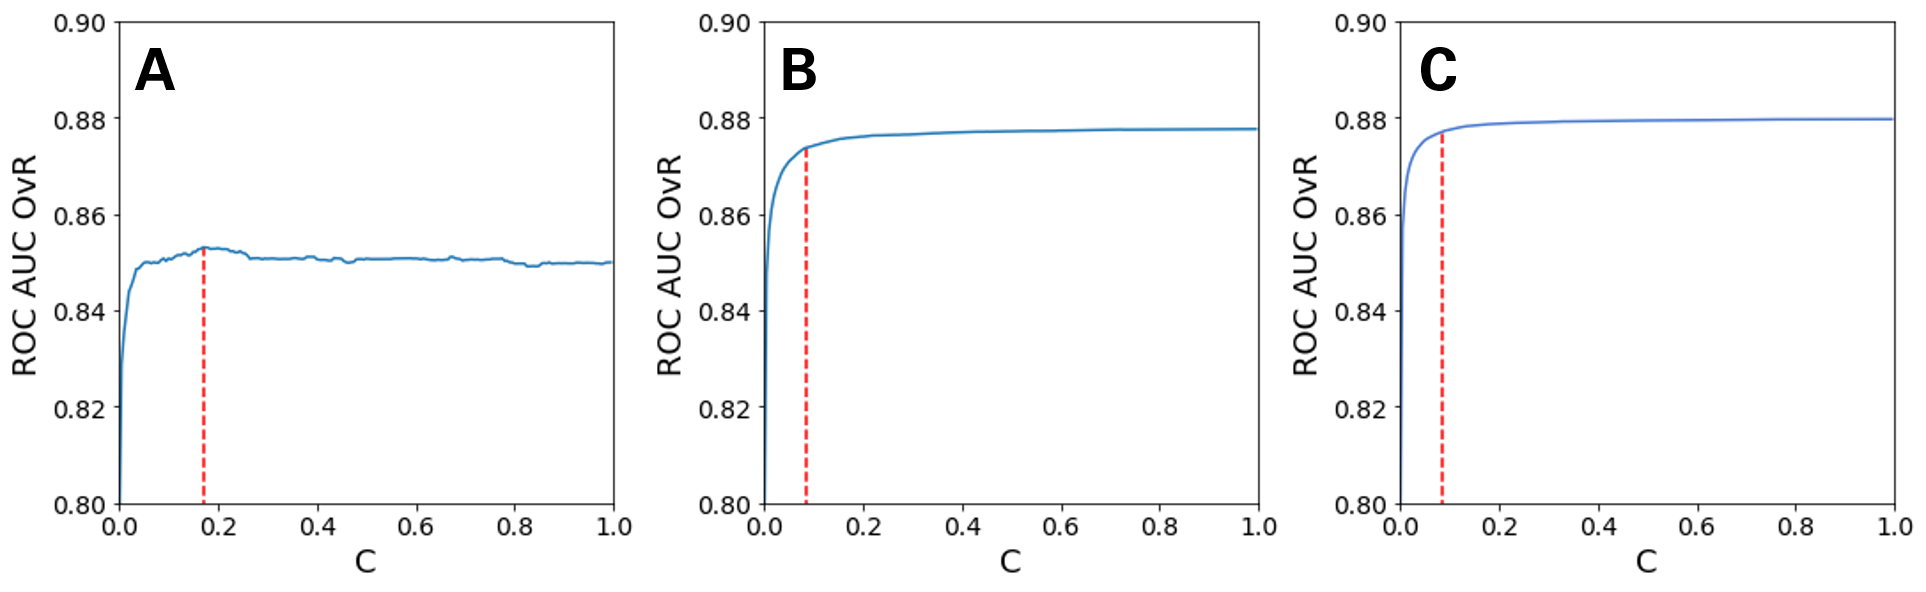
\includegraphics[width=\textwidth]{templates/images/Figure-LR_C_tuning.png}
\singlespacing
\caption[Logistic regression hyperparameter tuning]{Tuning plots for logistic regression \texttt{C} hyperparameter, based on ROC AUC OvR values for A.\ WDS,  B.\ WDS4, and C.\ WDS8. WDS value selected from the plot maximum. Selections for WDS4 and WDS8 target the elbow of the curve.}
\label{fig:logreg_hp_tuning}
\end{figure}

Out-of-sample AUC values calculated on the testing subset indicate that WDS4 has the best performance of the three data sets. Table \ref{tab:lr_coefficients} lists the feature coefficients for each of the four OvR classifiers that make up the multi-class LR model. Figure \ref{fig:logreg_coefs} illustrates these coefficients as a stacked bar chart, where each color bar depicts the magnitude of a coefficient for one of the OvR classifiers. The absolute length of the stacked bar for each feature, composed of the coefficient bars for all four classifiers, indicates the relative influence that feature has on the model prediction. Sorting the features by total stacked bar length quickly communicates the most important features for the logistic regression classifier: Si Geothermometer Temperature, Basement Depth, Drainage Density, Spring Density, and Volcanic-Dike Density.
\begin{table}[htp]
\resizebox{\textwidth}{!}{
\begin{tabular}{|l|r|r|r|r|}
\hline
 & \multicolumn{1}{l|}{\bftt{Class0 OvR}} & \multicolumn{1}{l|}{\bftt{Class1 OvR}} & \multicolumn{1}{l|}{\bftt{Class2 OvR}} & \multicolumn{1}{l|}{\bftt{Class3 OvR}} \\ \hline
\bftt{SiGeothermometry} & -0.81 & -0.17 & 0.33 & 0.65 \\ \hline
\bftt{BasementDepth} & -0.75 & -0.19 & 0.47 & 0.48 \\ \hline
\bftt{Drainage} & -0.61 & 0.19 & 0.66 & -0.25 \\ \hline
\bftt{Springs} & 0.28 & 0.02 & -0.83 & 0.53 \\ \hline
\bftt{VolcanicDikes} & -0.39 & 0.31 & 0.41 & -0.33 \\ \hline
\bftt{Boron} & -0.37 & 0.67 & -0.14 & -0.16 \\ \hline
\bftt{DEM} & 0.03 & 0.61 & -0.44 & -0.21 \\ \hline
\bftt{DosageRate} & -0.35 & 0.21 & -0.27 & 0.40 \\ \hline
\bftt{HeatFlow} & -0.08 & 0.31 & -0.49 & 0.26 \\ \hline
\bftt{StateFaults} & 0.19 & -0.54 & 0.09 & 0.26 \\ \hline
\bftt{CrustalThickness} & 0.14 & 0.40 & -0.30 & -0.24 \\ \hline
\bftt{Vents} & 0.54 & -0.15 & -0.29 & -0.10 \\ \hline
\bftt{StrainRate} & 0.14 & -0.50 & 0.27 & 0.08 \\ \hline
\bftt{Earthquakes} & -0.09 & 0.35 & -0.40 & 0.14 \\ \hline
\bftt{QFaults} & 0.13 & 0.34 & 0.00 & -0.47 \\ \hline
\bftt{Lithium} & 0.30 & -0.47 & 0.05 & 0.12 \\ \hline
\bftt{Precipitation} & 0.21 & 0.20 & -0.19 & -0.22 \\ \hline
\bftt{Gravity} & 0.12 & 0.24 & -0.29 & -0.08 \\ \hline
\bftt{WTGrad} & 0.02 & -0.26 & 0.25 & -0.01 \\ \hline
\bftt{GravityGrad} & 0.14 & -0.14 & 0.10 & -0.10 \\ \hline
\bftt{WTDepth} & 0.10 & -0.10 & 0.13 & -0.13 \\ \hline
\bftt{Magnetic} & 0.16 & 0.03 & 0.00 & -0.19 \\ \hline
\bftt{MagneticGrad} & -0.04 & -0.03 & -0.01 & 0.09 \\ \hline
\bftt{DEMGrad} & -0.02 & -0.07 & 0.03 & 0.05 \\ \hline
\end{tabular}}
\caption[Multi-class logistic regression classifier coefficients]{Feature coefficients for each of the four OvR classifiers that make up the multi-class logistic regression classifier for WDS4. Values are rounded to the nearest hundredth for display purposes.}
\label{tab:lr_coefficients}
\end{table}
\begin{figure}
\centering
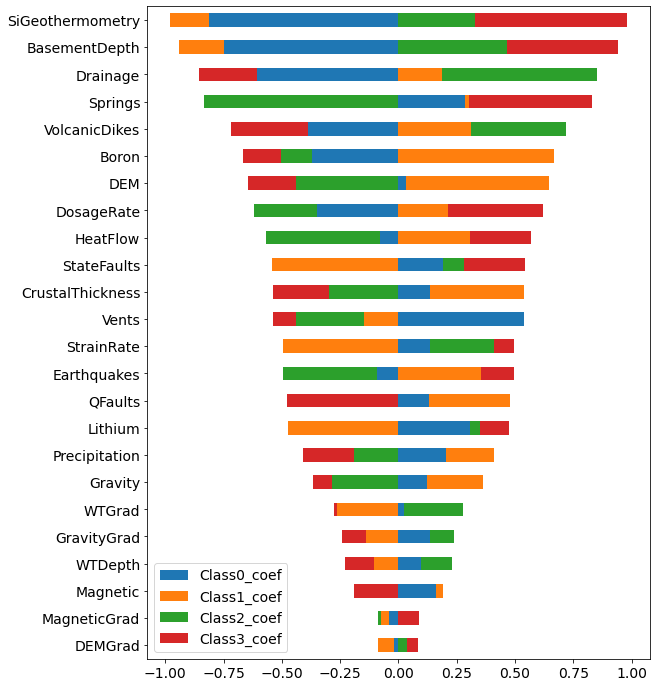
\includegraphics[width=\textwidth]{templates/images/Figure-LR-coefficients.png}
\singlespacing
\caption[Logistic regression feature coefficients]{Stacked bar chart of logistic regression coefficient values for OvR classifiers trained on WDS4. Values are also listed in Table \ref{tab:lr_coefficients}. Coefficient bars are color-coded by individual classifier. Total stacked bar length for a feature is a proxy for overall importance of that feature to the classification.}
\label{fig:logreg_coefs}
\end{figure}

\subsection{Feature Selection} \label{ch5:lr_feature_selection}

Figure \ref{fig:logreg_rfe} presents the results of Recursive Feature Selection (RFE, see Section \ref{ch3:lr_rfe}) applied to the LR model for WDS4. Based on the plot, a local peak in AUC occurs when 18 features are used. Adding the remaining features results in small gains in AUC, but with diminishing returns for six additional features of complexity. Using this threshold, the data layers removed from the model include: DEM Gradient, Gravity Gradient, Magnetic Anomaly, Magnetic-Anomaly Gradient, Water-Table Depth, and Average Precipitation. Note that Average Precipitation appears higher on the coefficients plot (Figure \ref{fig:logreg_coefs}) than other features that were not removed. Since RFE iteratively removes predictors and refits the model, relative coefficients can change, particularly if there was collinearity with a removed variable.

\begin{figure}
\centering
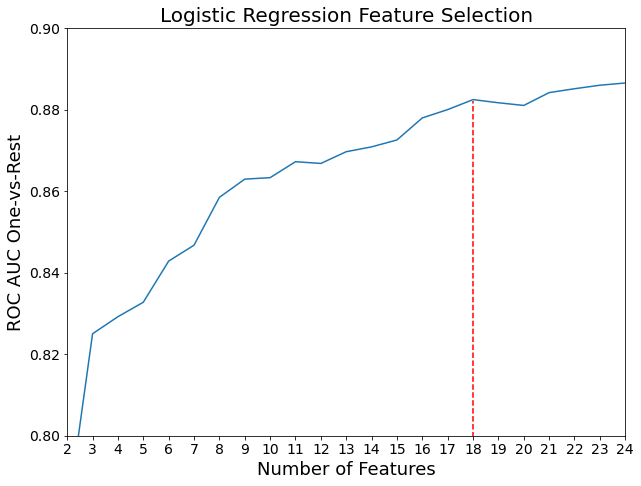
\includegraphics[width=0.70\textwidth]{templates/images/Figure-LR_feature_selection.png}
\singlespacing
\caption[Logistic regression feature selection]{Logistic regression feature selection using RFE and WDS4. Red dashed line indicates the chosen number of features to use for the LR model.}
\label{fig:logreg_rfe}
\end{figure}

\subsection{Optimized Model Results}\label{ch5:lr_final_results}

\begin{figure}
\centering
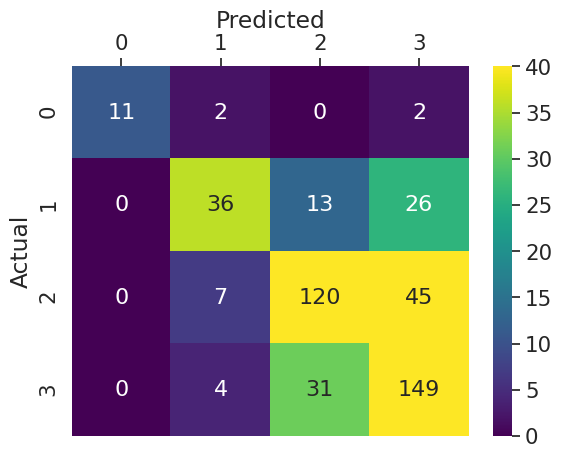
\includegraphics[width=0.5\textwidth]{templates/images/Figure-LR-ConfusionMatrix.png}
\singlespacing
\caption[Logistic regression confusion matrix]{Confusion matrix for the tuned LR model trained on WDS4.}
\label{fig:logreg_conf_matrix}
\end{figure}

A final LR model trained on WDS4 was constructed using the tuned \verb|C| hyperparameter and reduced feature set from RFE. The confusion matrix shows moderately good model performance (Figure \ref{fig:logreg_conf_matrix}). Correct predictions (TP) for each of the four classes of geothermal gradient outnumber the misclassifications (FP) for those classes. The model appears to struggle most with differentiating between class-2 mid-grade (40--60 K/km) and class-3 high-grade (> 60 K/km) gradient locations ($31+45$ misclassifications), although there are also a large number (26) of false high-grade assignments to class-1 low-grade gradient points.

Figure \ref{fig:logreg_auc} plots the macro average, micro average, and individual class ROC curves. Class-0 (non-thermal) predictive ability is quite high, pulling the micro-average AUC up to 0.88.  The macro AUC value of 0.85 is more aligned with the performance for other classes, which range over an AUC of 0.79--0.83. The trade-off between class 2 and class 3 is apparent in how the curve shapes mirror each other approximately, with respect to the anti-diagonal line TPR = 1 $-$ FPR.

\begin{figure}[!htp]
\centering
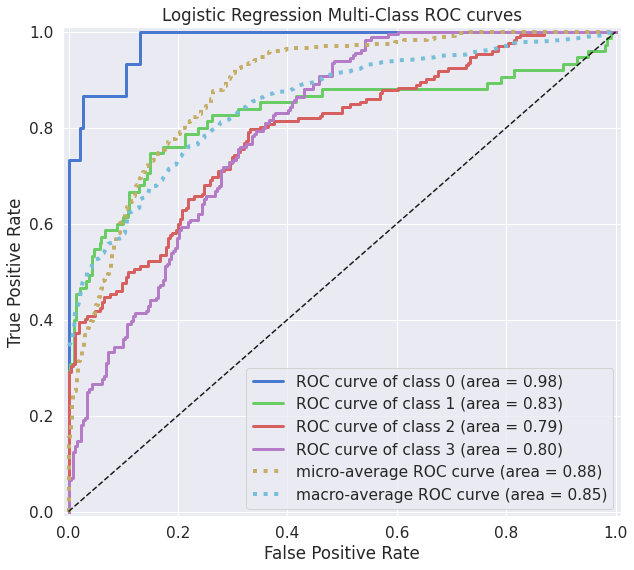
\includegraphics[width=0.9\textwidth]{templates/images/Figure-LR-AUC.png}
\singlespacing
\caption[Logistic regression ROC curves]{ROC curves for the tuned LR model trained on WDS4.}
\label{fig:logreg_auc}
\end{figure}

Model predictions for the study area are generated by passing the FDS through the final trained model. Class predictions are plotted in Figure \ref{fig:logreg_final_map}. High-grade geothermal-gradient patches are concentrated to the southeast and through the center of the AOI. Smaller high-grade regions are observed along the southwest state boundary, following the Rio Grande to the northeast, and a smaller patch directly to the north. Comparing this result to the Southwestern NM PFA geothermal-gradient data layer from \citet{bielicki_hydrogeolgic_2015}, high-grade predictions match in general spatial location except for the predicted patches to the north. The LR model tends to predict more widespread and spatially-continuous high-grade regions, while under-predicting lower gradient regions to the north (Colorado Plateau), east (Great Plains), and mid-AOI near the Rio Grande, compared to the PFA layer. Recall the PFA geothermal gradient layer is an interpolated layer from well data and not ground-truth (see Section \ref{app:dl_geothermal_gradient}). Here it simply serves as a convenient reference for comparison.

\begin{figure}[!htp]
\centering
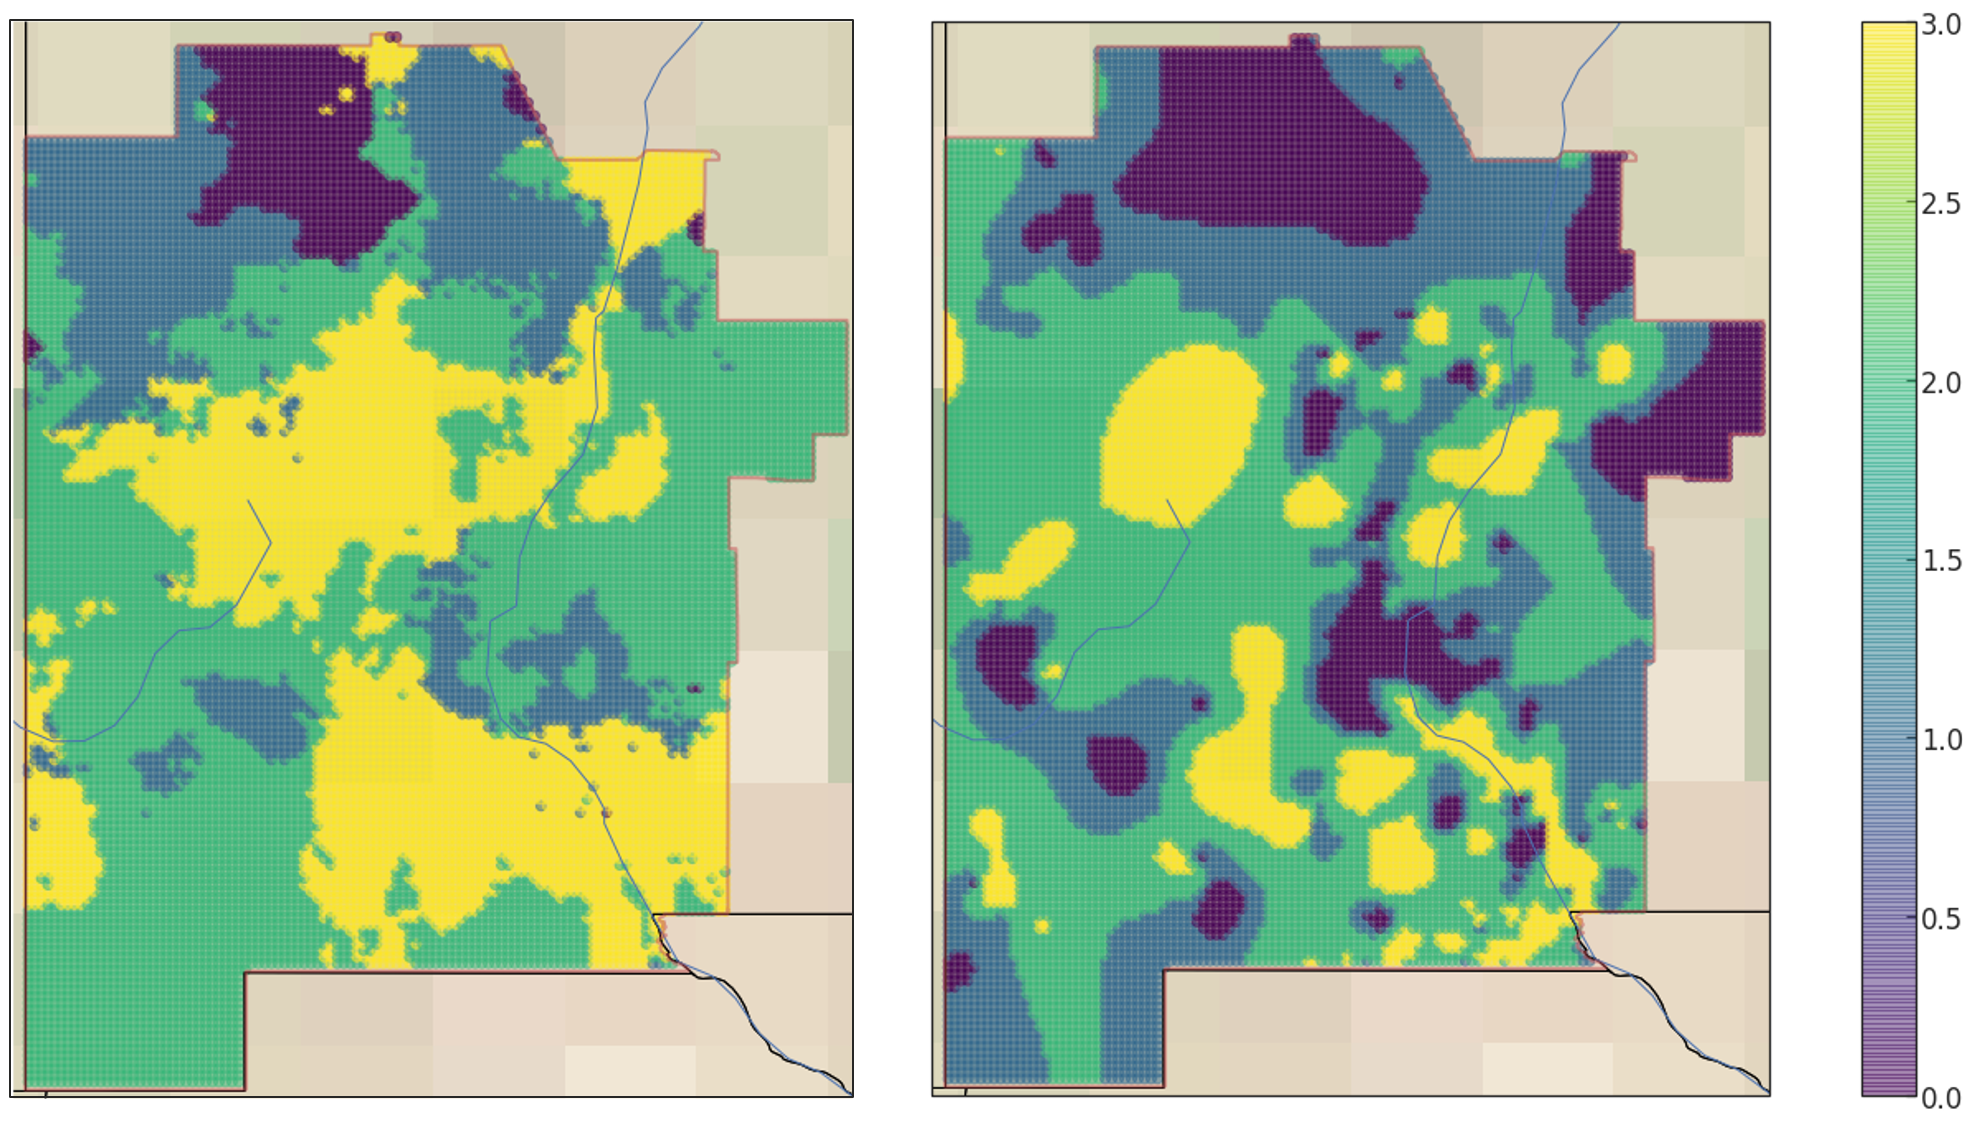
\includegraphics[width=\textwidth]{templates/images/Figure-LR-FinalMap_Joint.png}
\caption[Logistic regression prediction map]{Left: Map predictions of geothermal-gradient class from the tuned LR model trained on WDS4. Right: geothermal-gradient feature layer from Southwestern NM PFA study \protect\citep{bielicki_hydrogeolgic_2015}.}
\label{fig:logreg_final_map}
\end{figure}

\section{Decision Trees}\label{ch5:dtree_model}

\subsection{Hyperparameter Tuning}\label{ch5:dtree_tuning}

Stepping up in complexity, the scikit-learn version of the decision tree (DT) classifier has over ten adjustable hyperparameters for tuning performance \citep{pedregosa_scikit-learn_2011}. Here, six hyperparameters are tuned using the stratified $k$-fold CV method described in Section \ref{ch3:strat_kfold_cv}, with 10 folds and the multi-class OvR ROC AUC scoring metric. The tuning process relied on defaults for the scikit-learn \textit{DecisionTreeClassifier} to define initial values until a specific hyperparameter was tuned. Figures below illustrate the tuning results for the WDS4 data set.

First, \verb|max_depth| and \verb|criterion| were tuned together. \verb|max_depth| limits tree expansion by capping the number of parameter evaluations (tree nodes) considered before a classification label assignment. \verb|criterion| refers to the quality metric used for tree construction, i.e., Gini index or Entropy. The similarity of AUC curves in Figure \ref{fig:dtree_maxdepth} illustrates a relative insensitivity to \verb|criterion|, while \verb|max_depth| plays a stronger role in classifier performance. A maximum AUC score is observed with a \verb|max_depth| of 8 and \verb|criterion| choice of Entropy.

\begin{figure}[!htp]
\centering
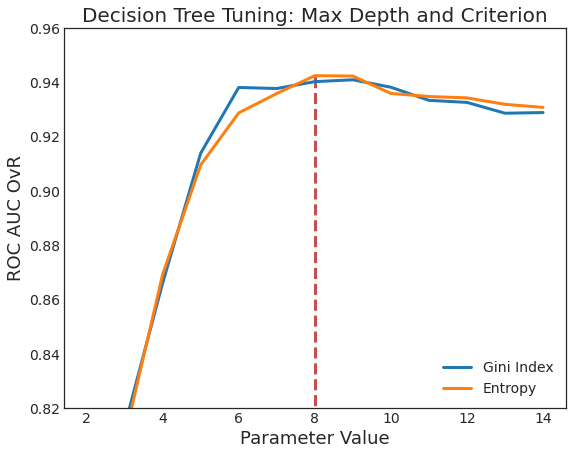
\includegraphics[width=.6\textwidth]{templates/images/Figure-DT_tuning_maxdepth_criterion.png}
\caption[Decision tree max depth tuning]{Results from stratified $k$-fold cross validation tuning of the \texttt{max\_depth} and \texttt{criterion} hyperparameters using WDS4. The red dashed line indicates the selected \texttt{max\_depth} value.}
\label{fig:dtree_maxdepth}
\end{figure}

Next, \verb|min_samples_leaf| and \verb|min_samples_split| were tuned in succession. The former defines the minimum number of samples from the training set that must be assigned to a leaf node for that leaf to remain in the tree. The latter sets a minimum number of training-set samples that must be assigned to a node before that node can be considered for a split. Figure \ref{fig:dtree_min_samples} illustrates the selected hyperparameter values, defined by maxima in the AUC vs.\ hyperparameter value plots. The insensitivity of the classifier to low values of \verb|min_samples_split| demonstrates the cascading influence of the hyperparameters in this tuning flow. When \verb|min_samples_leaf| is set to 8, a split can only occur when the node being split has at least 16 observations, so any \verb|min_samples_split| value under 16 does not influence tree construction. 

\begin{figure}[!htp]
\centering
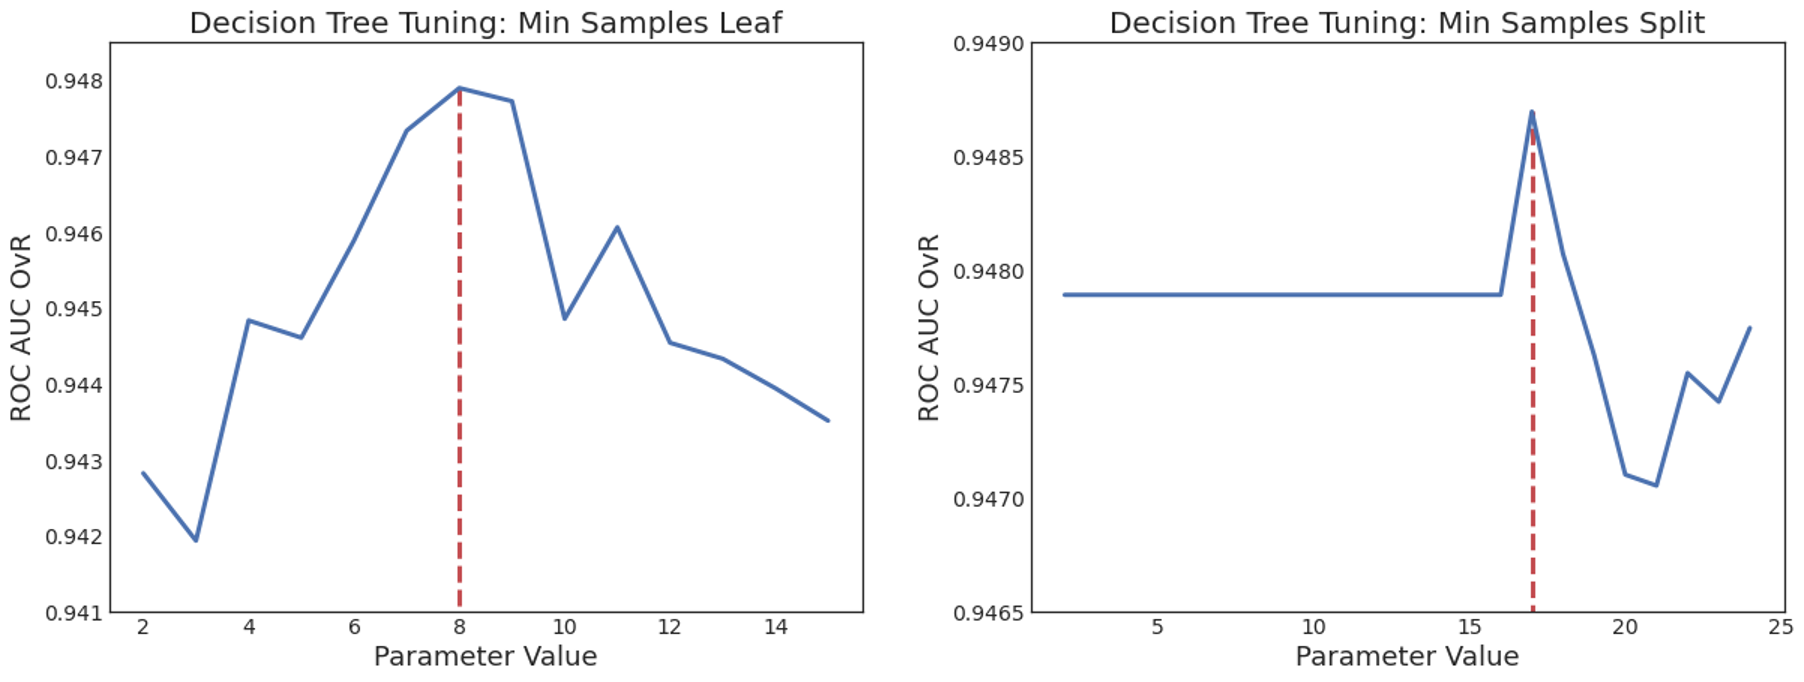
\includegraphics[width=\textwidth]{templates/images/Figure-DT_tuning_min_samp_leaf_split.png}
\caption[Decision tree min samples tuning]{Results from stratified $k$-fold cross validation tuning of the \texttt{min\_samples\_leaf} (Left) and \texttt{min\_samples\_split} (Right) hyperparameters using WDS4. The red dashed lines indicate the selected values.}
\label{fig:dtree_min_samples}
\end{figure}

One optimization trick when training DT models is to consider only a subset of the features when splitting decision tree nodes. This also adds an element of randomness to tree construction because decision trees can differ when constructed on the same training data depending on which features were considered for each split. No clear maximum appears in the AUC plot for \verb|max_features| (Figure \ref{fig:dtree_max_features}), so a value of 8 was selected using the elbow criterion. \verb|max_features| can also cause problems when performing feature selection if the feature count drops below the \verb|max_features| value, so care must be taken in using this hyperparameter.

\begin{figure}[!htp]
\centering
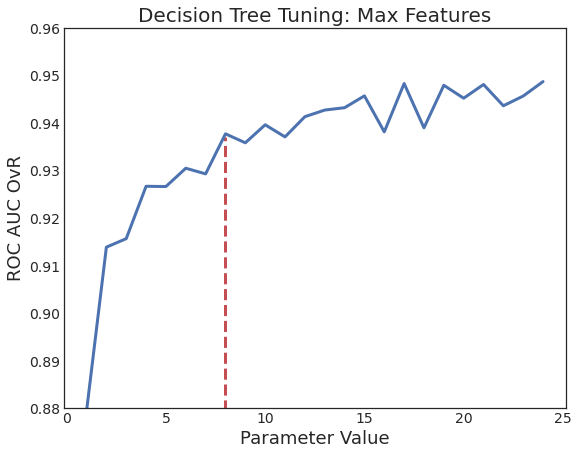
\includegraphics[width=.6\textwidth]{templates/images/Figure-DT_tuning_max_features.png}
\caption[Decision tree max features tuning]{Results from stratified $k$-fold cross validation tuning of the \texttt{max\_features} hyperparameter using WDS4. The red dashed line indicates the selected value, conservatively selected at the high end of the ``elbow'' in the plot.}
\label{fig:dtree_max_features}
\end{figure}

The final hyperparameter, \verb|ccp_alpha|, controls the trade-off between model fit and complexity during the tree-pruning backward pass of tree construction. As the alpha value increases from zero, the difference between in-sample (training) and out-of-sample (validation) performance decreases, but so does the overall performance of the classifier on the validation subset. Figure \ref{fig:dtree_alpha} shows a clear minimum in train-validate AUC difference, however the validation-set performance drops from 0.95 to under 0.85 when using this value for \verb|ccp_alpha|. The default value of \verb|ccp_alpha| = 0.0 is chosen instead to maximize out-of-sample AUC.

\begin{figure}[!htp]
\centering
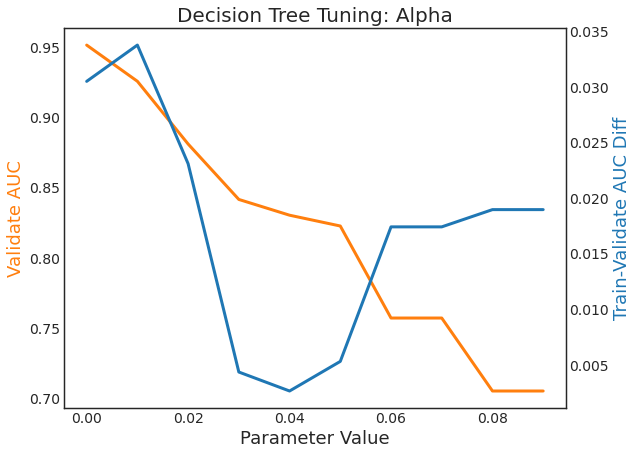
\includegraphics[width=.6\textwidth]{templates/images/Figure-DT_tuning_alpha.png}
\caption[Decision tree alpha tuning]{Results from stratified $k$-fold cross validation tuning of the \texttt{ccp\_alpha} hyperparameter. The orange line plots the validation subset AUC. The blue line plots the difference in AUC between training and validation subsets.}
\label{fig:dtree_alpha}
\end{figure}

Final hyperparameter values and performance results for WDS, WDS4, and WDS8 are listed in Table \ref{tab:dtree_tuning}. The data imputation strategy used to create WDS4 and WDS8 results in a significant improvement in classifier performance over the original WDS.

\begin{table}[!htp]
\centering
\begin{tabular}{l|c|c|c|}
\cline{2-4}
                                          & \textbf{WDS} & \textbf{WDS4} & \textbf{WDS8} \\ \hline
\multicolumn{1}{|l|}{\bftt{criterion}}           & Gini & Entropy & Entropy \\ \hline
\multicolumn{1}{|l|}{\bftt{max\_depth}}          & 5    & 8    & 10   \\ \hline
\multicolumn{1}{|l|}{\bftt{min\_samples\_leaf}}  & 7    & 8    & 10   \\ \hline
\multicolumn{1}{|l|}{\bftt{min\_samples\_split}} & 21   & 17   & 24   \\ \hline
\multicolumn{1}{|l|}{\bftt{max\_features}}       & 5    & 8    & 6    \\ \hline
\multicolumn{1}{|l|}{\bftt{ccp\_alpha}}          & 0    & 0    & 0    \\ \hline
\multicolumn{1}{|l|}{\bftt{Accuracy$_{train}$}}  & 0.767 & 0.881 & 0.880 \\ \hline
\multicolumn{1}{|l|}{\bftt{Accuracy$_{test}$}}   & 0.600 & 0.818 & 0.838 \\ \hline
\multicolumn{1}{|l|}{\bftt{AUC$_{train}$}}       & 0.909 & 0.982 & 0.985 \\ \hline
\multicolumn{1}{|l|}{\bftt{AUC$_{test}$}}        & 0.814 & 0.944 & 0.961 \\ \hline
\end{tabular}
\caption[Decision tree hyperparameter tuning results]{Tuned hyperparameter selections and resulting decision-tree model Accuracy and AUC for training and testing subsets of WDS, WDS4, and WDS8.}
\label{tab:dtree_tuning}
\end{table}

\subsection{Feature Selection}\label{ch5:dtree_feat_selection}

Figure \ref{fig:dtree_feat_import} shows the feature importances determined by models constructed using WDS, WDS4, and WDS8. Features are sorted on the sum of importance values across all 3 data sets. Although differences exist, Si Geothermometer Temperature tops the list as the most important predictor in all cases. And the bottom six features are also remarkably consistent across data sets: Water-Table Depth, Water-Table Gradient, Gravity-Anomaly Gradient, Magnetic Anomaly, Magnetic-Anomaly Gradient, and DEM Gradient. Dropping these features reduces the count to 18 features in total.

\begin{figure}[!htp]
\centering
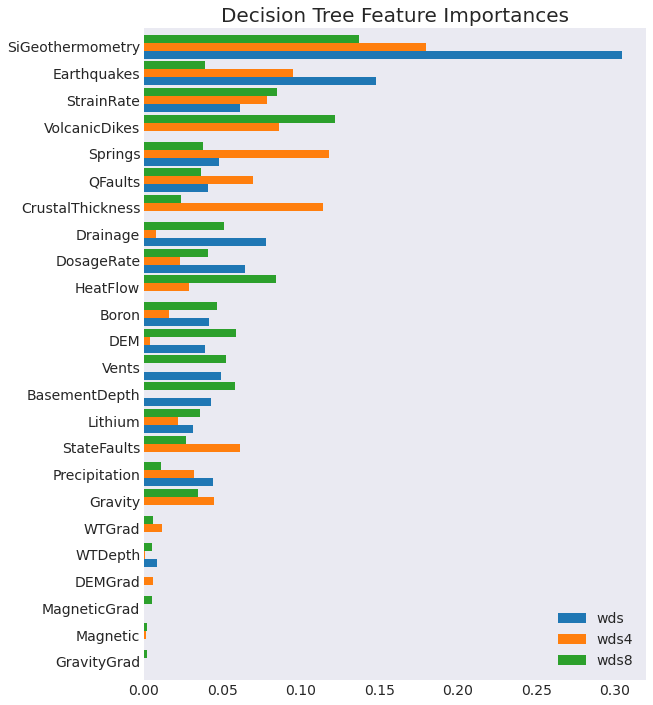
\includegraphics[width=\textwidth]{templates/images/Figure-DT_feature_importances_all.png}
\caption[Decision tree feature importances]{Decision tree feature importances for WDS, WDS4, and WDS8, sorted on the sum total importance across the 3 data sets.}
\label{fig:dtree_feat_import}
\end{figure}

\subsection{Optimized Model Results}\label{dtree_final_results}

\begin{figure}
\centering
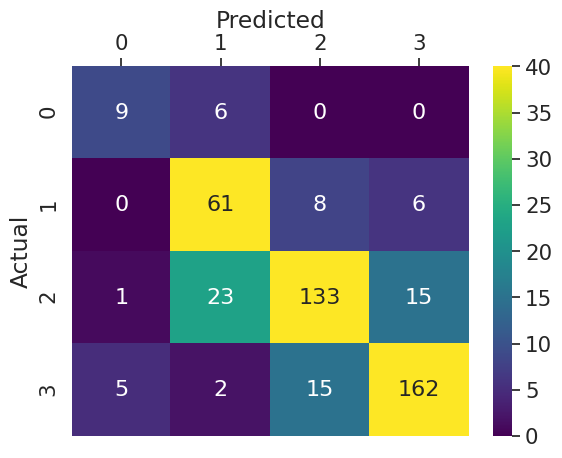
\includegraphics[width=0.5\textwidth]{templates/images/Figure-DT-ConfusionMatrix.png}
\singlespacing
\caption[Decision tree confusion matrix]{Confusion matrix for the tuned DT model trained on WDS4.}
\label{fig:dtree_conf_matrix}
\end{figure}

A final DT model trained on WDS4 was constructed using the tuned hyperparameters and 18-predictor reduced feature set. The confusion matrix (Figure \ref{fig:dtree_conf_matrix}) demonstrates an improvement in model results over the logistic-regression method. Low-grade gradient locations are correctly predicted for almost double the number of sites, and half as many misclassifications are observed between class-2 (mid-grade) and class-3 (high-grade) geothermal gradients than with the LR model.

Figure \ref{fig:dtree_auc} shows the macro average, micro average, and individual class DT ROC curves. All individual class AUC values exceed 0.90. Class 0 (non-thermal) continues to demonstrate the highest predictive performance (AUC = 0.97), but class-3 (high-grade) predictive ability boosts the micro-average AUC at higher decision thresholds, i.e., where the class-0 ROC curve steeply drops in TPR for FPR < 0.1. Class-2 (medium-grade) classification performance lags behind all other classes for the DT classifier.

\begin{figure}
\centering
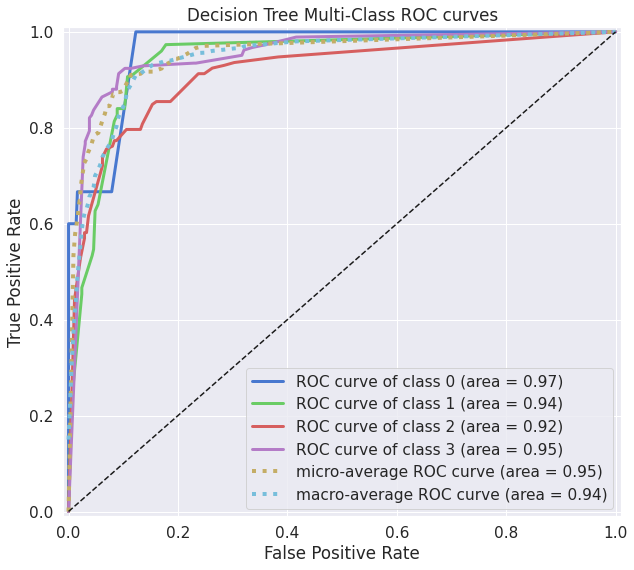
\includegraphics[width=0.6\textwidth]{templates/images/Figure-DT_AUC.png}
\caption[Decision tree ROC curves]{ROC curves for the tuned DT model trained on WDS4.}
\label{fig:dtree_auc}
\end{figure}

Model predictions for the study area are generated by passing the FDS through the DT model. Class assignments are plotted in Figure \ref{fig:dtree_final_map}. The high-grade geothermal gradient patches to the southeast and central regions of the AOI are not as broad and continuous as in the LR model (Figure \ref{fig:logreg_final_map}). Predictions for low-grade gradient or non-thermal areas are concentrated to the NW (Colorado Plateau) and central-east (Rio Grade Rift-Great Plains transition). The overall distribution of geothermal gradient classes is similar to the \citet{bielicki_hydrogeolgic_2015} PFA layer (Figure \ref{fig:dtree_final_map}) but with a greater apportionment of high-grade gradient areas and fewer low-grade or non-thermal locations in the DT model.

\begin{figure}
\centering
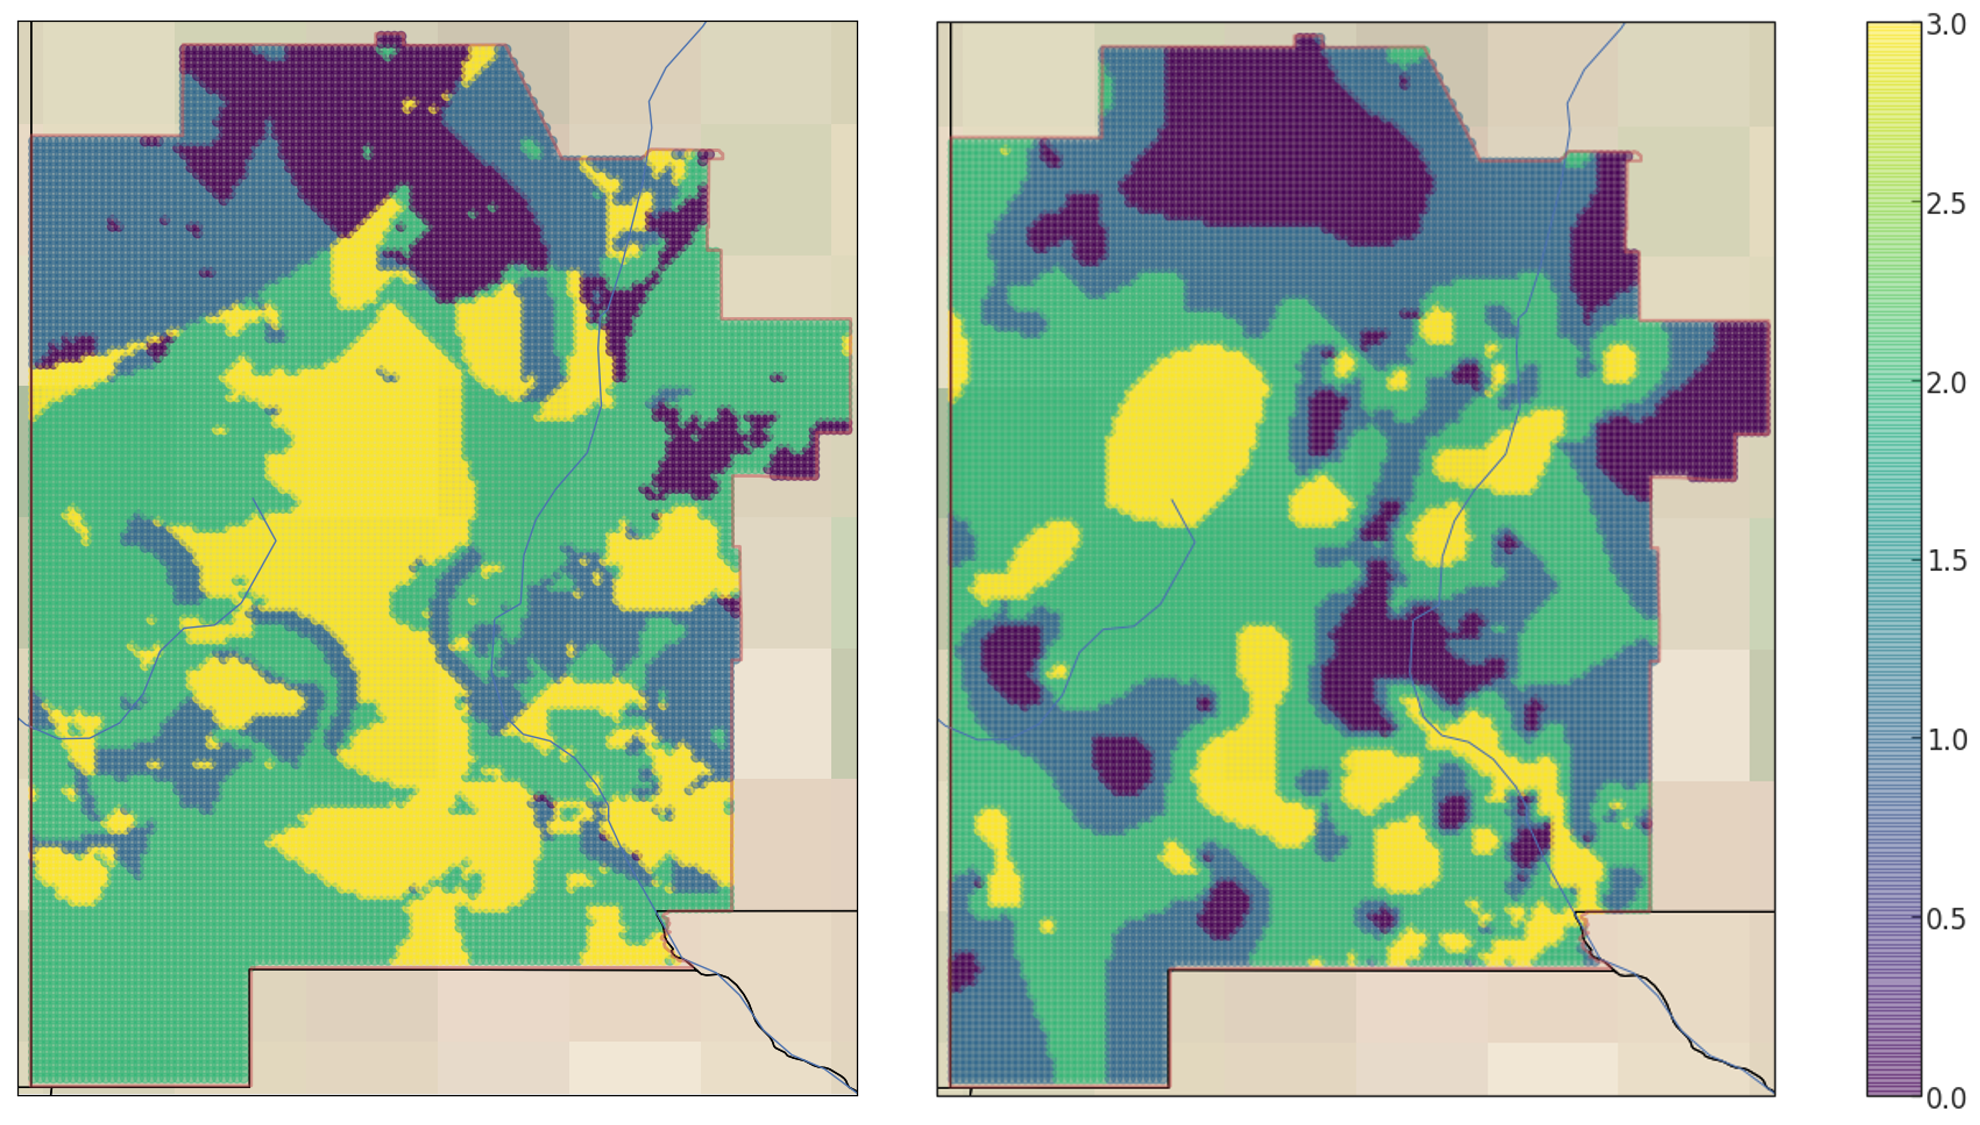
\includegraphics[width=\textwidth]{templates/images/Figure-DT-FinalMap_Joint.png}
\caption[Decision tree prediction map]{Left: Map predictions of geothermal gradient class from the tuned DT model trained on WDS4. Right: geothermal gradient feature layer from Southwestern NM PFA study \protect\citep{bielicki_hydrogeolgic_2015}}
\label{fig:dtree_final_map}
\end{figure}

Note that if the random seed (fixed in the present study for solution repeatability) is free to change and new DT models are constructed, some of the characteristics of this DT prediction will also change. In fact, one downside of the DT model is this randomness; decision trees will structurally rearrange each time the algorithm is run, even on the same training data, due to randomness in the node splitting process. Nevertheless, tree performance remains relatively stable overall. And the ability to plot and visually step through the model makes it one of the most accessible and interpretable methods to use (see Figure \ref{fig:dtree_viz}).

\begin{figure}[!htp]
\centering
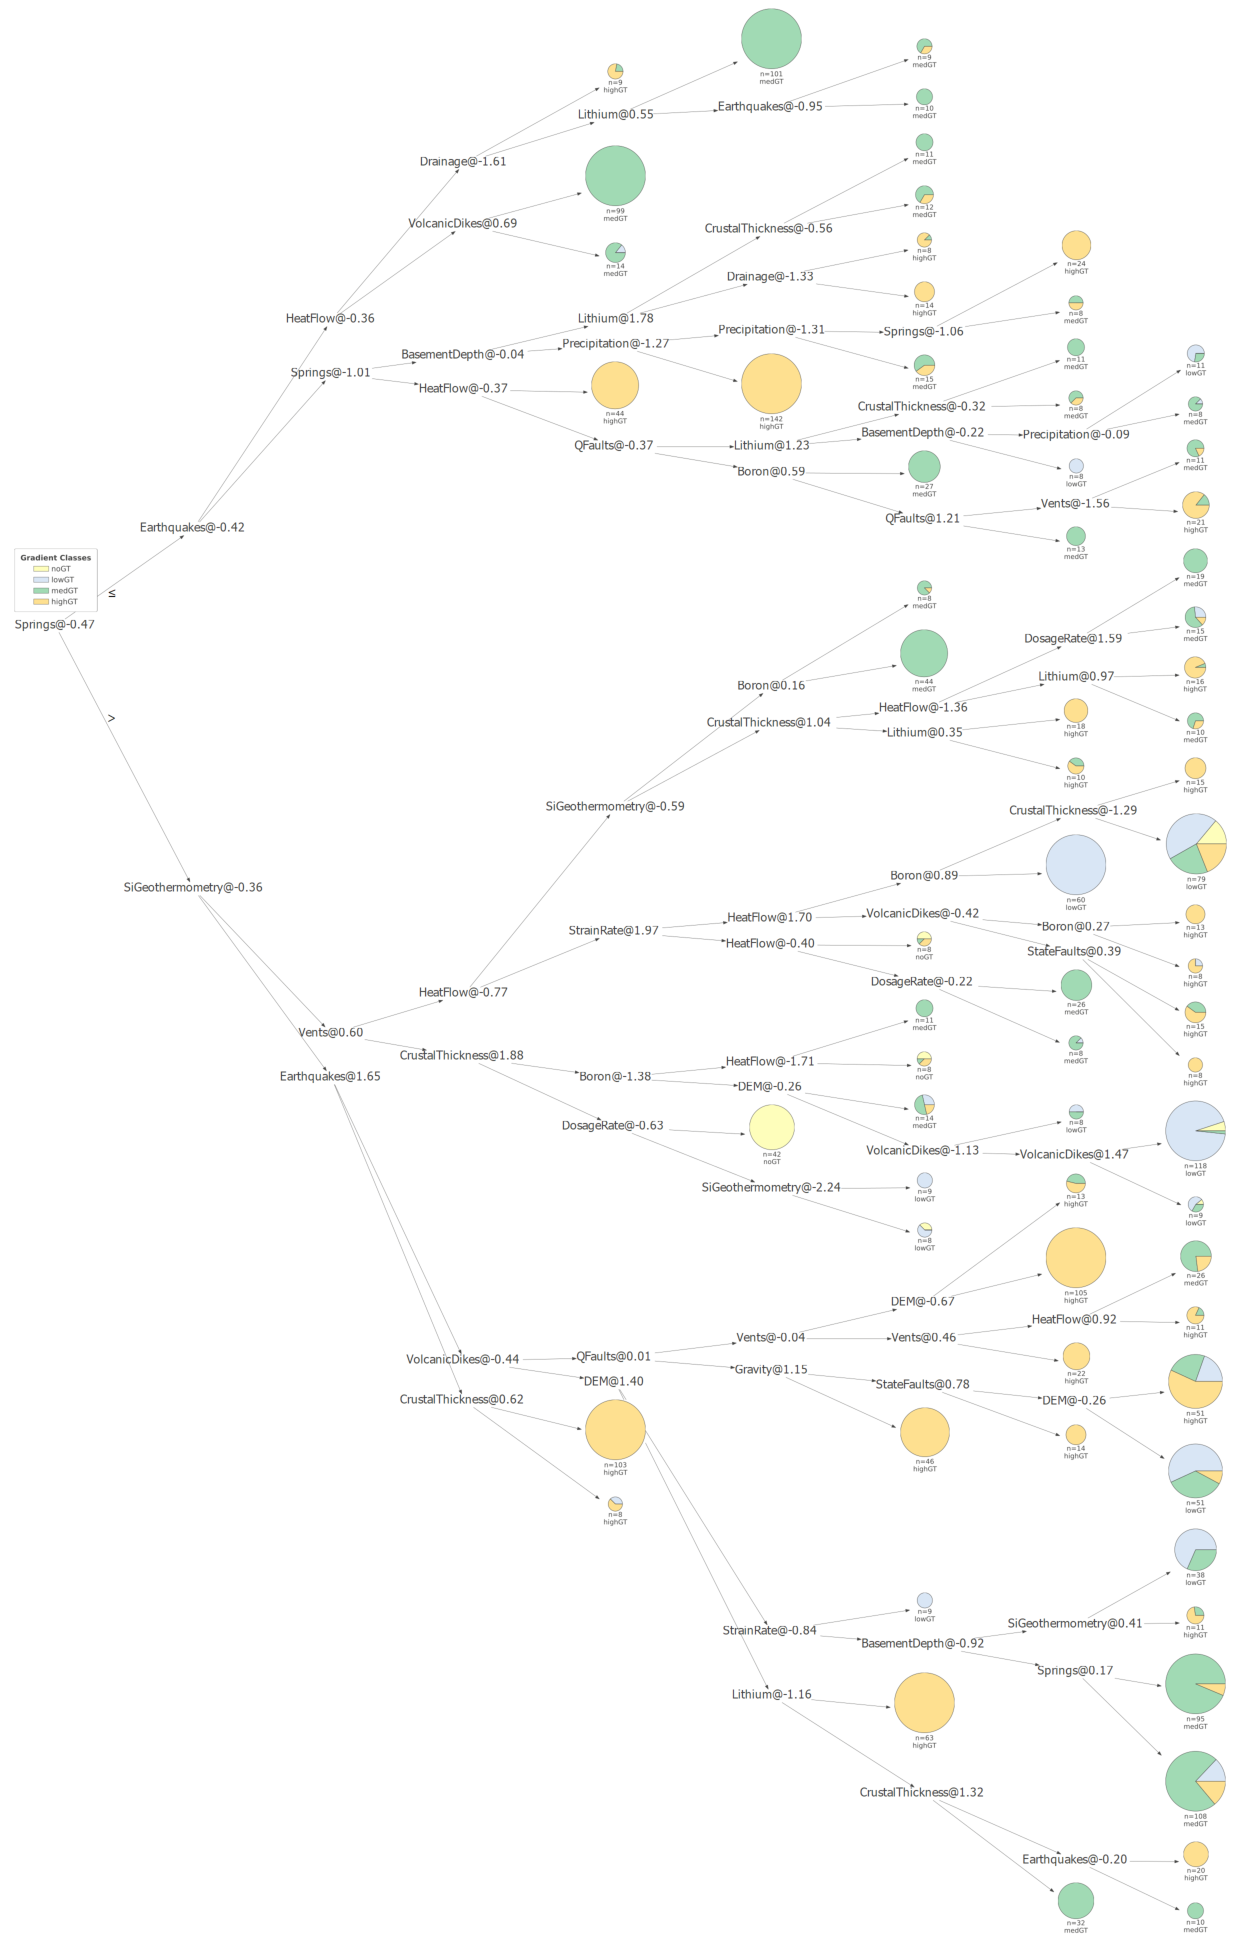
\includegraphics[height=0.85\textheight,keepaspectratio]{templates/images/Figure-DT_viz_portrait.pdf}
\caption[Decision tree visualization]{Decision-tree visualization for the final decision-tree model. Nodes are noted by predictor labels with their decision threshold. Bubbles illustrate the final distribution of classes in a leaf node, sized by number of observations. The majority class determines the classification label.}
\label{fig:dtree_viz}
\end{figure}

\section{Tree Ensembles (XGBoost)}\label{ch5:xgb_model}

\subsection{Hyperparameter Tuning}\label{ch5:xgb_tuning}

XGBoost comes with many of the same hyperparameters as decision trees, plus additional parameters related to boosting and optimization. With so many hyperparameters, tuning the model becomes a time-consuming and complex process. The method followed here was adapted from an online tutorial covering the topic \citep{jain_xgboost_2016}.

The following hyperparameters were tuned for the final model:
\begin{itemize}[itemsep=2pt]
    \item \textbf{Maximum depth}: same as the \verb|max_depth| hyperparameter for decision trees, restricts how deep each tree can grow during construction. Initially set to 5.
    \item \textbf{Minimum child weight}: sets a minimum weight requirement for a leaf node during the backward-pass pruning process. Similar to \verb|min_samples_leaf| in decision trees, except this uses the XGBoost-specific weights ($\theta$) noted in equation \ref{eq:xgb_objective}. Initially set to 1.0.
    \item \textbf{Gamma}: defines a minimum reduction in the loss function necessary for a split to be preserved during tree pruning. Initially set to 0.2.
    \item \textbf{Learning rate}: a.k.a.\ shrinkage factor, scales the impact of each tree on the boosted model prediction, i.e., the $\alpha_s$ in equation \ref{eq:xgb_form}. Initially set to 0.01.
    \item \textbf{Lambda}: L2 regularization term on the leaf scores, i.e., the $\lambda$ in equations \ref{eq:xgb_objective} and \ref{eq:xgb_obj_simple}. Initially set to 1.0.
    \item \textbf{Subsample}: defines the fraction of observations in the full training set that are randomly selected as a limited training set for each tree. Initially set to 1.0.
    \item \textbf{Column sample by tree}: sets the fraction of predictors in the full training set that are randomly selected as a limited feature set for constructing each tree. Initially set to 1.0.
    \item \textbf{Number of estimators}: controls the number of sequential trees in the model, i.e., $B$ in equation \ref{eq:xgb_form}. Initially set to 200.
    \item \textbf{Scale positive weight}: scales the gradient for the positive class to influence model corrections during training, helping manage imbalanced classification. Initially set to 1.0.
\end{itemize}

The preferred tuning method for XGBoost is the cross-validation strategy described in Section \ref{ch3:strat_kfold_cv}. Since this method uses the input data to both train and validate, the pre-generated training and validation subsets (Table \ref{tab:stratified_split_counts}) were re-combined before using CV. An initial trial-and-error testing of different hyperparameter combinations found the best starting values for \verb|learning_rate| and \verb|n_estimators| were 0.01 and 200, respectively. Higher learning rates like those suggested by \citet{jain_xgboost_2016} led to a nearly perfect-fitting model before hyperparameters could be tuned, and more estimators created undesirably long training times. In the figures and discussion that follow, results are described for WDS4. Full results for all three data sets are provided in Table \ref{tab:xgb_tuning}.

\begin{figure}[!htp]
\centering
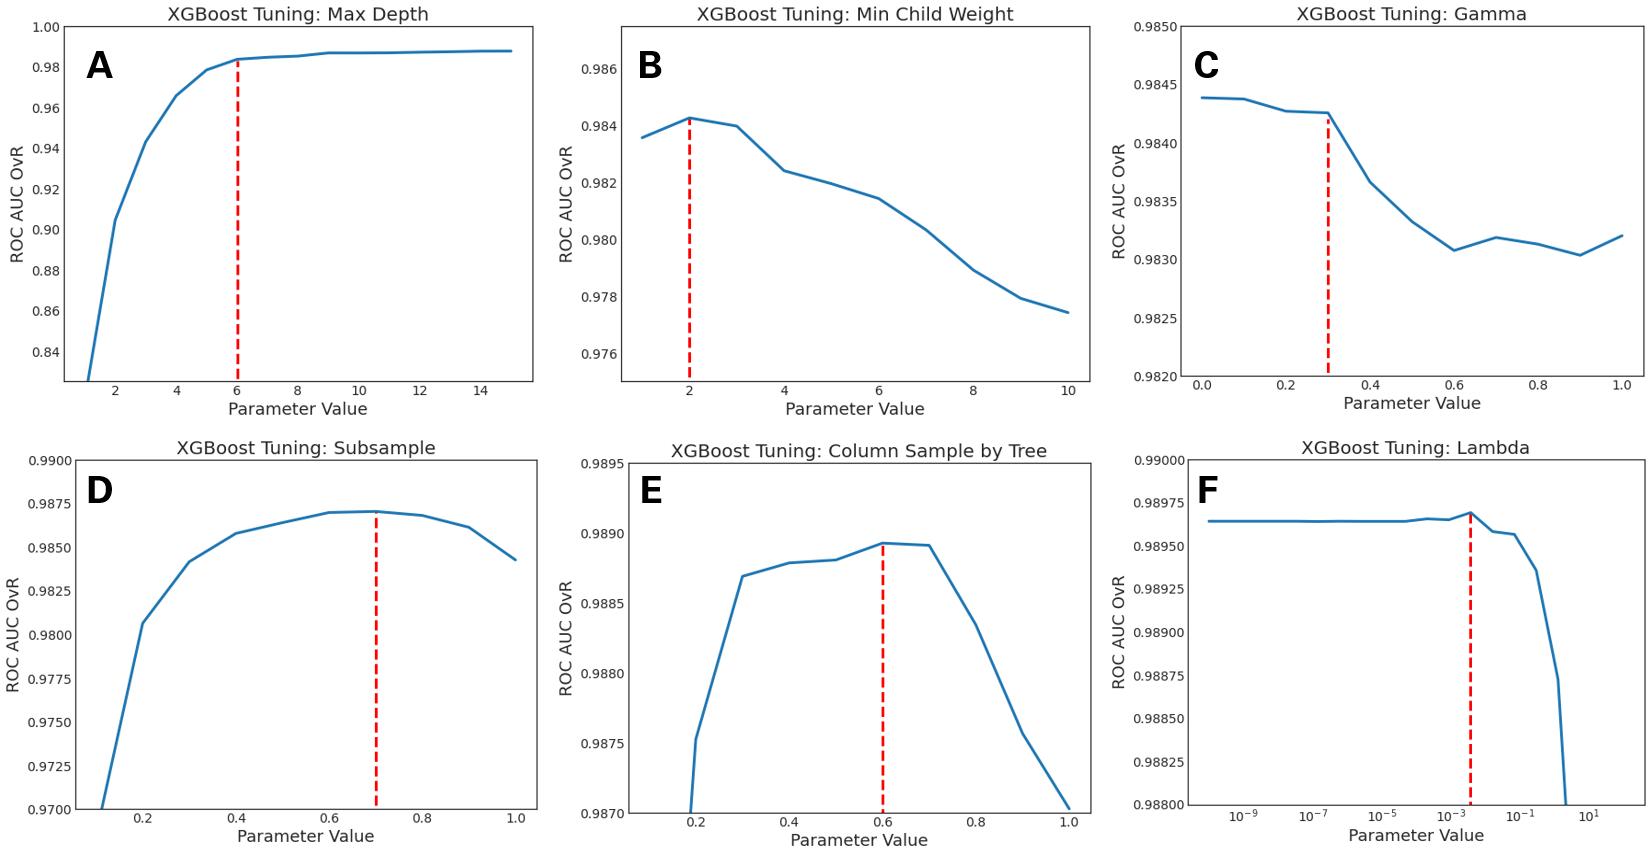
\includegraphics[width=\textwidth]{templates/images/Figure-XGB_Hyperparameters.png}
\caption[XGBoost hyperparameter tuning]{Hyperparameter tuning results for XGBoost modeling. A.\ \bftt{max\_depth}, B.\ \bftt{min\_child\_weight}, C.\ \bftt{gamma}, D.\ \bftt{subsample}, E.\ \bftt{colsample\_bytree}, F.\ \bftt{lambda}. Red dashed lines indicate values selected for the final model.}
\label{fig:xgb_hyperparam}
\end{figure}

XGBoost hyperparameters were tuned in succession using stratified 10-fold CV and a grid search across potential hyperparameter values. Figure \ref{fig:xgb_hyperparam}A shows the results for \verb|max_depth|. As noted when tuning the DT model (Section \ref{ch5:dtree_tuning}), \verb|max_depth| does not exhibit a clear maximum in the AUC vs.\ hyperparameter value plot. A preferred value of 6 was selected to ensure sufficient tree performance while balancing tree complexity.

Next, tuning was performed on the \verb|min_child_weight| hyperparameter. Results of the stratified 10-fold CV method revealed a clear maximum AUC when \verb|min_child_weight| is 2 (Figure \ref{fig:xgb_hyperparam}B).

XGBoost uses a default value of 0 for the \verb|gamma| hyperparameter, which controls when tree partitioning should stop based on loss reduction. Cross-validation shows nearly level AUC values out to \verb|gamma| = 0.3, after which the AUC score quickly drops. This threshold value was selected for the model (Figure \ref{fig:xgb_hyperparam}C).

Trees in the XGBoost model can be trained on random subsets of training data observations and individual feature columns. Tuning of \verb|subsample| identified a broad maximum in AUC when using 60--80\% of the training observations to build decision trees (Figure \ref{fig:xgb_hyperparam}D). The selected \verb|subsample| value is 70\%. For \verb|colsample_bytree|, the best AUC results occur when 60\% of the features are included in the training (Figure \ref{fig:xgb_hyperparam}E). A value below 100\% for \verb|colsample_bytree| suggests that removing features based on importance estimates could be beneficial, as previously discussed for both logistic regression (Section \ref{ch5:lr_feature_selection}) and decision trees (Section \ref{ch5:dtree_feat_selection}). A more robust method for feature attribution and selection using Shapley values is considered in Section \ref{ch5:xgb_feature_selection}.

Tuning results show model AUC remains flat, then quickly drops for increasing values of the \verb|lambda| hyperparameter (Figure \ref{fig:xgb_hyperparam}F). This behavior shows how higher levels of regularization can cause data underfitting. The largest \verb|lambda| value just short of this drop-off was selected for the final model.

\verb|scale_pos_weight| was similarly tuned, but AUC results remained unchanged for all hyperparameter values tested. The multi-class XGBoost classifier appears to be insensitive to this hyperparameter.

As a final step in model tuning, \verb|learning_rate| was decreased to 0.005 and \verb|n_estimators| increased to 1000. Using the slower learning rate reduces the chance of overfitting the training data, while the increased number of sequential trees in the model ensures a good fit can be learned. Final hyperparameter values and performance results for WDS, WDS4, and WDS8 are listed in Table \ref{tab:xgb_tuning}. Once again, WDS4 and WDS8 out-perform the original WDS based on AUC values for the test set.

\begin{table}
    \centering
    \begin{tabular}{l|c|c|c|}
    \cline{2-4}
                                             & \textbf{WDS}   & \textbf{WDS4}    & \textbf{WDS8}  \\ \hline
    \multicolumn{1}{|l|}{\bftt{max\_depth}}         & 6     & 6       & 6     \\ \hline
    \multicolumn{1}{|l|}{\bftt{min\_child\_weight}} & 2     & 2       & 5     \\ \hline
    \multicolumn{1}{|l|}{\bftt{gamma}}              & 0.5   & 0.3     & 0.5   \\ \hline
    \multicolumn{1}{|l|}{\bftt{subsample}}          & 0.8   & 0.7     & 0.7   \\ \hline
    \multicolumn{1}{|l|}{\bftt{colsample\_bytree}}  & 0.4   & 0.6     & 0.6   \\ \hline
    \multicolumn{1}{|l|}{\bftt{reg\_lambda}}        & 0.30  & 0.0038 & 1.3   \\ \hline
    \multicolumn{1}{|l|}{\bftt{scale\_pos\_weight}} & 0.0   & 0.0     & 0.0   \\ \hline
    \multicolumn{1}{|l|}{\bftt{learning\_rate}}     & 0.005 & 0.005   & 0.005 \\ \hline
    \multicolumn{1}{|l|}{\bftt{n\_estimators}}      & 1000  & 1000    & 1500  \\ \hline
    \multicolumn{1}{|l|}{\bftt{Accuracy$_{train}$}} & 0.995 & 0.991   & 0.988 \\ \hline
    \multicolumn{1}{|l|}{\bftt{Accuracy$_{test}$}}  & 0.767 & 0.944   & 0.955 \\ \hline
    \multicolumn{1}{|l|}{\bftt{AUC$_{train}$}}      & 1.000 & 1.000   & 1.000 \\ \hline
    \multicolumn{1}{|l|}{\bftt{AUC$_{test}$}}       & 0.938 & 0.995   & 0.995 \\ \hline
    \end{tabular}
    \caption[XGBoost hyperparameter tuning results]{Tuned hyperparameter selections and resulting XGBoost model Accuracy and AUC for training and test subsets of WDS, WDS4, and WDS8.}
    \label{tab:xgb_tuning}
\end{table}

\subsection{Feature Selection}\label{ch5:xgb_feature_selection}

\begin{figure}
\centering
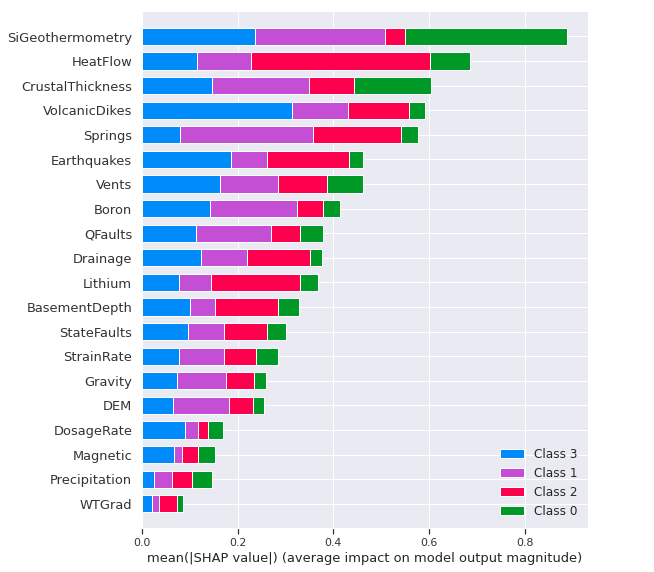
\includegraphics[width=\textwidth]{templates/images/Figure-Shapley_notitle.png}
\caption[XGBoost SHAP variable importance]{SHAP variable importance plot for the XGBoost classifier, derived using the testing data subset of WBS4. Colors illustrate feature importances for specific classes of geothermal gradient. The sum of colored bar lengths indicates overall feature importance for the model. Nearby values in sorted stacked bar length suggest the model has five key predictive features, eleven features with moderate influence on the model, and four features with low predictive value.}
\label{fig:xgb_shap_global}
\end{figure}

Section \ref{ch3:xgb_shapley} noted several desirable attributes of feature importances derived from Shapley analysis. Figure \ref{fig:xgb_shap_global} plots the results of SHAP value calculations for the WDS4 XGBoost classifier. Recall that SHAP values have local significance on a per-observation basis (i.e., local accuracy). This plot illustrates the mean absolute SHAP value of each feature across all instances in the test data subset, giving an average global impact. The colored bars illustrate relative importance of that feature in the prediction for the respective geothermal gradient class. Global importance is indicated by the sum of colored bar lengths (stacked length) for each feature. The order of the features is sorted on stacked length to highlight both the most and least important features. The top five most important features for the WDS4 model include Si Geothermometer Temperature, Heat Flow, Crustal Thickness, Volcanic-Dike Density, and Spring Density. Features not shown in the plot were deemed to have zero predictive value (i.e., DEM Gradient, Gravity Gradient, Magnetic-Anomaly Gradient, and Water-Table Depth). The lowermost four features on the plot ---Gamma Ray Absorbed-Dose Rate, Magnetic Anomaly, Average Precipitation, and Water-Table Gradient --- are also selected for elimination, reducing the final feature set for the XGBoost model to sixteen predictors.

\subsection{Optimized Model Results}\label{ch5:xgb_final_results}

A final XGBoost model parameterized with the tuned hyperparameter values (Table \ref{tab:xgb_tuning}) was trained on the reduced sixteen-feature version of WDS4. The resulting confusion matrix (Figure \ref{fig:xgb_conf_matrix}) demonstrates why XGBoost receives best-in-class praise as a predictive model. Test set accuracy for WDS4 is 94\%. The largest number of misclassifications ($6+6$) occur between high-grade (class 3) and medium-grade (class 2) geothermal gradient. Ten additional locations are mistakenly labeled low-grade (class 1) for medium-grade or vice-versa. Only two test set locations were off by more than one consecutive class.

\begin{figure}[!htp]
\centering
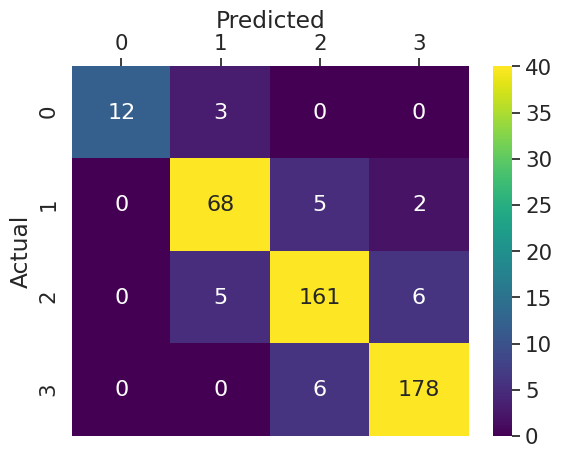
\includegraphics[width=0.5\textwidth]{templates/images/Figure-XGB16-ConfusionMatrix.png}
\singlespacing
\caption[XGBoost confusion matrix]{Confusion matrix for the tuned XGBoost model trained on WDS4.}
\label{fig:xgb_conf_matrix}
\end{figure}
\pagebreak
Figure \ref{fig:xgb_auc} shows the macro average, micro average, and individual class XGBoost ROC curves. All individual class AUC values are at or above 0.99. This is close to an ideal ROC plot for a classifier.

\begin{figure}[htp]
\centering
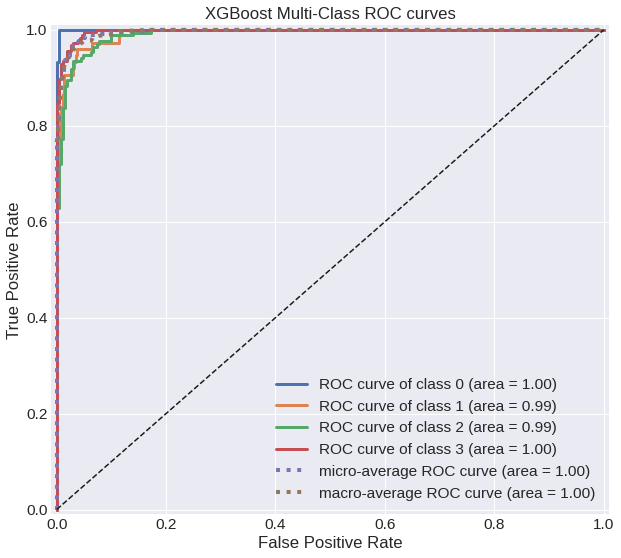
\includegraphics[width=.6\textwidth]{templates/images/Figure-XGB16-AUC.png}
\caption[XGBoost ROC curves]{ROC curves for tuned XGBoost model trained on WDS4.}
\label{fig:xgb_auc}
\end{figure}

Geothermal gradient predictions for the study area are generated by passing the FDS through the XGBoost model, as shown in Figure \ref{fig:xgb_final_map}. High-grade gradient areas to the southeast and central regions of the AOI align with the class 3 locations in the \citet{bielicki_hydrogeolgic_2015} Southwestern NM PFA map. XGBoost predicts more spatially continuous and connected high-grade regions, with a limited number of isolated patches to the southwest and on the northern section of the Rio Grande. Both maps have a similar non-thermal class 0 region to the north (Colorado Plateau), but they differ most significantly midway along the Rio Grande, to the southwest (Basin and Range), and in the eastern panhandle (Great Plains) where the PFA map predicts low-grade gradient or non-thermal classifications.

\begin{figure}[!htp]
\centering
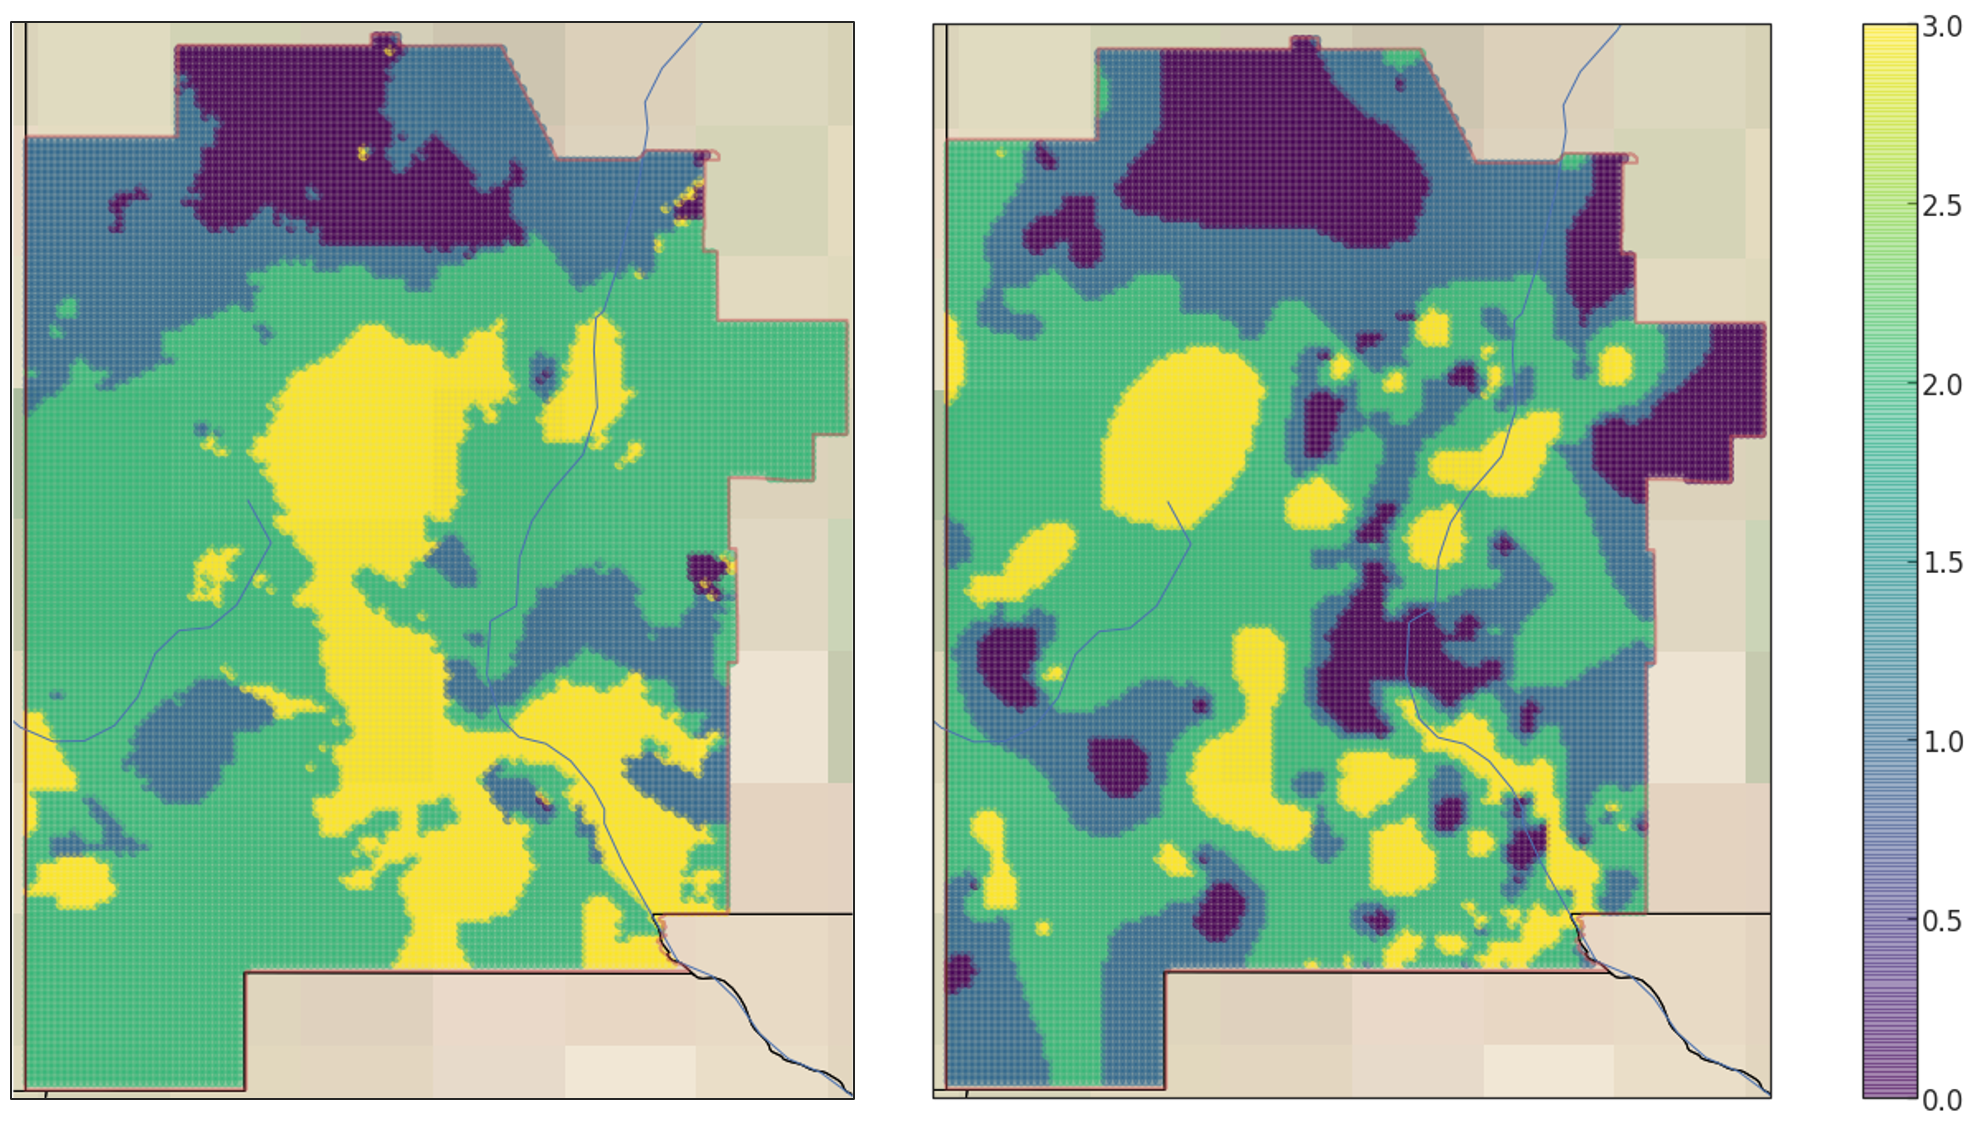
\includegraphics[width=\textwidth]{templates/images/Figure-XGB-FinalMap_Joint.png}
\caption[XGBoost prediction map]{Left: Map predictions of geothermal gradient from the tuned XGBoost model trained on WDS4. Right: geothermal gradient feature layer from Southwestern NM PFA study \protect\citep{bielicki_hydrogeolgic_2015}.}
\label{fig:xgb_final_map}
\end{figure}

\section{Neural Networks}\label{ch5:ann_model}

\subsection{Network Architecture}\label{ch5:ann_structure}

\begin{figure}[!htp]
\centering
\begin{minipage}[b][][b]{.35\linewidth}
    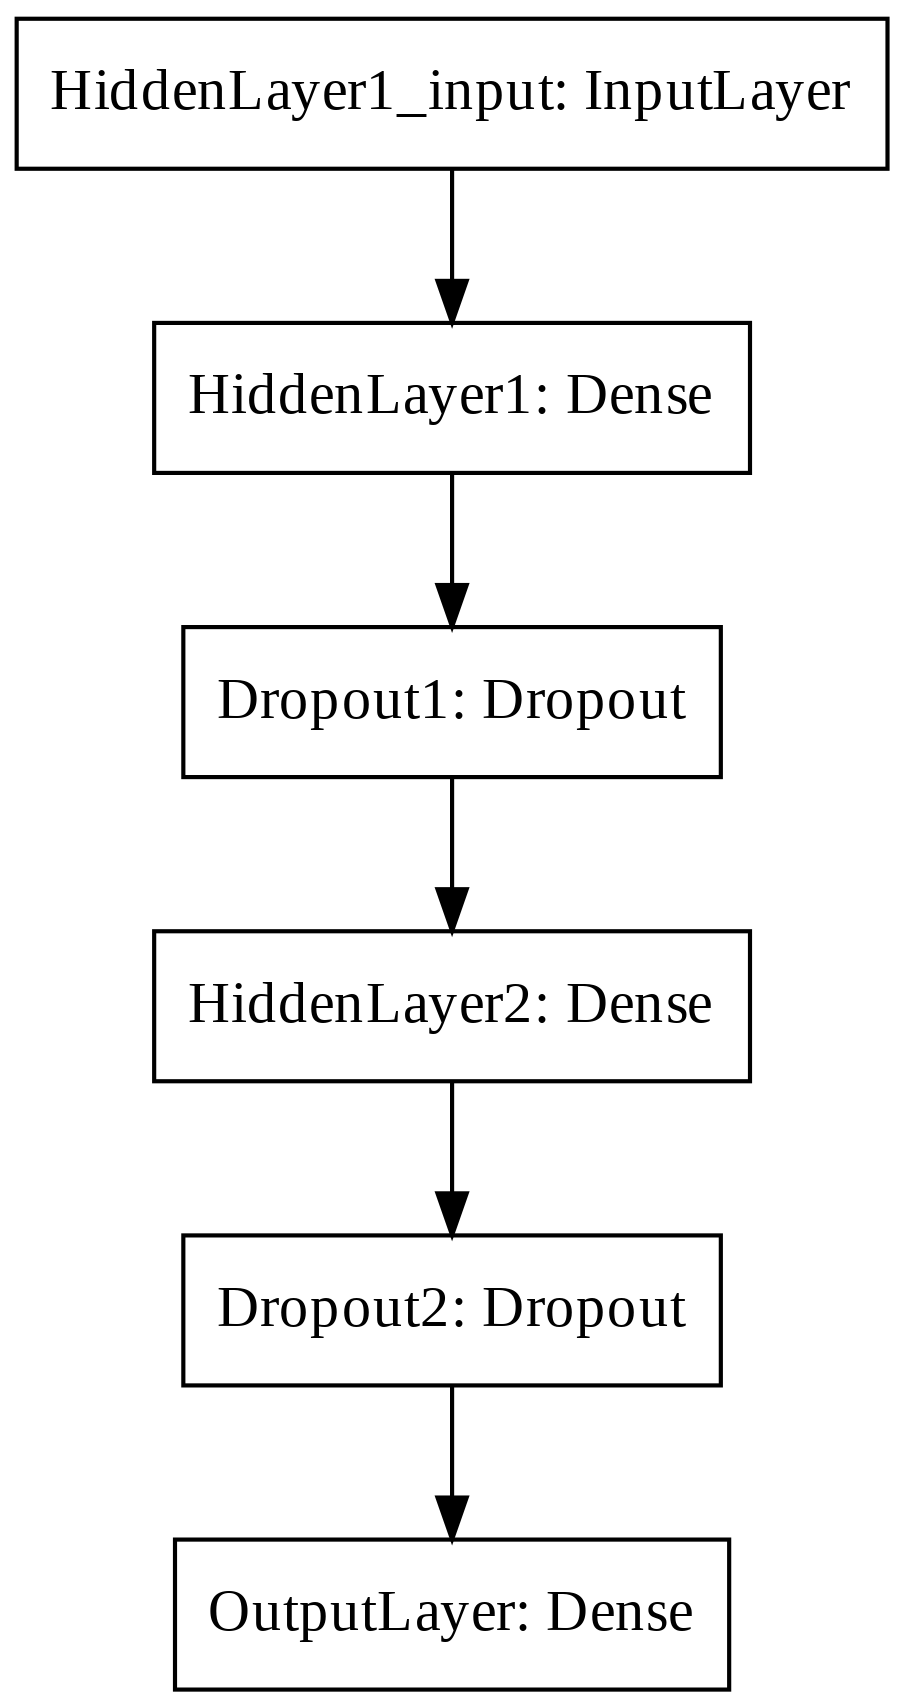
\includegraphics[width=\linewidth]{templates/images/Figure-TF_NN_Structure.png}
    \caption[Neural network structural flow]{Structural flow chart for the TensorFlow-based neural networks.}
    \label{fig:nn_text_structure}
\end{minipage}
\hfill
\begin{minipage}[b][][b]{.61\linewidth}
    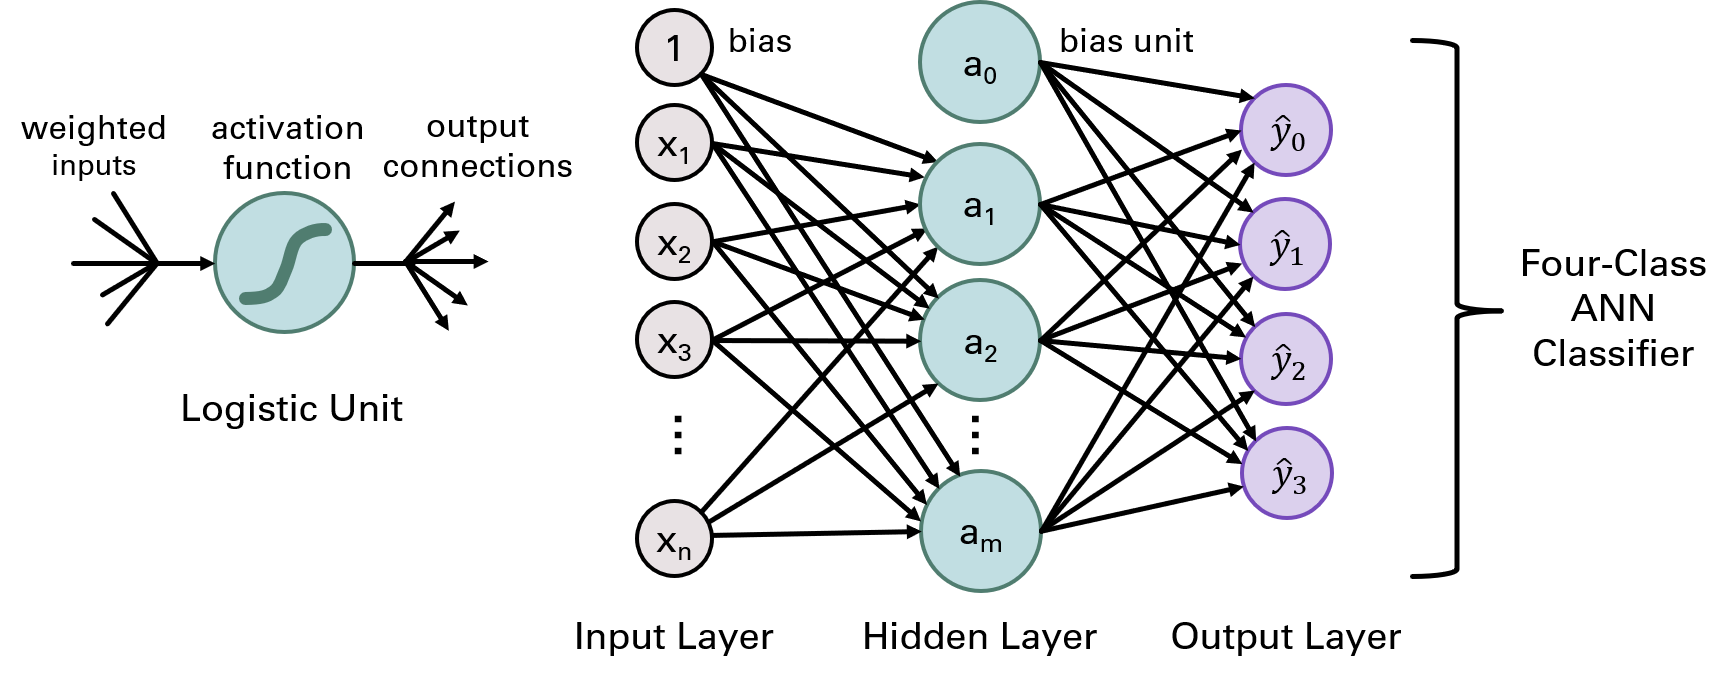
\includegraphics[width=\linewidth]{templates/images/Figure-ANN.png}
    \caption[Neural network structural schematic]{Schematic diagram of the artificial neural networks. Not shown are the dropout operations after each hidden layer.}
    \label{fig:nn_dot_structure}
\end{minipage}
\end{figure}

This thesis uses a neural network constructed using TensorFlow \citep{abadi_tensorflow_2016} to test geothermal gradient classification performance for the Southwestern NM study area. The network design is a 4-layer structure starting with an input layer of size \({(1\times24)}\), followed by two hidden layers sized ($1\times24$), and ending in a four-class output layer ($1\times4$) (Figures \ref{fig:nn_text_structure}, \ref{fig:nn_dot_structure}). Layer sizes assume all original features except Average Air Temperature (see Section \ref{ch3:feat_corr}) are included in the training. In addition, the network applies dropout after each of the hidden layers. Dropout helps prevent overfitting by randomly assigning inputs to zero, temporarily severing a defined percentage of node connections (a hyperparameter) during each step of the training process.

\subsection{Hyperparameter Tuning}\label{ch5:ann_tuning}

Tuning of the network focuses on five key hyperparameters:
\begin{itemize}[itemsep=2pt]
    \item \textbf{Learning rate}: controls the magnitude of adjustments to the network weights during each step of the training process. The Adam optimizer adjusts this rate during training, so the value here defines a starting learning rate. Initially set to 0.001.
    \item \textbf{Lambda ($\lambda$)}: the L2 weight regularization term, i.e., the $\lambda$ in equation \ref{eq:nn_cost_function}. Initially set to $1\times10^{-4}$.
    \item \textbf{Batch size}: the number of training samples included in each mini-batch when calculating training gradients for updating the network weights. Initially set to one tenth the number of samples.
    \item \textbf{Dropout rate}: the fraction of network connections zeroed-out during each step of the training process. Initially set to 0.2.
    \item \textbf{Number of epochs}: the number of training repetitions when fitting the model to the data. Initially set to 100.
\end{itemize}

\begin{figure}[htp]
\centering
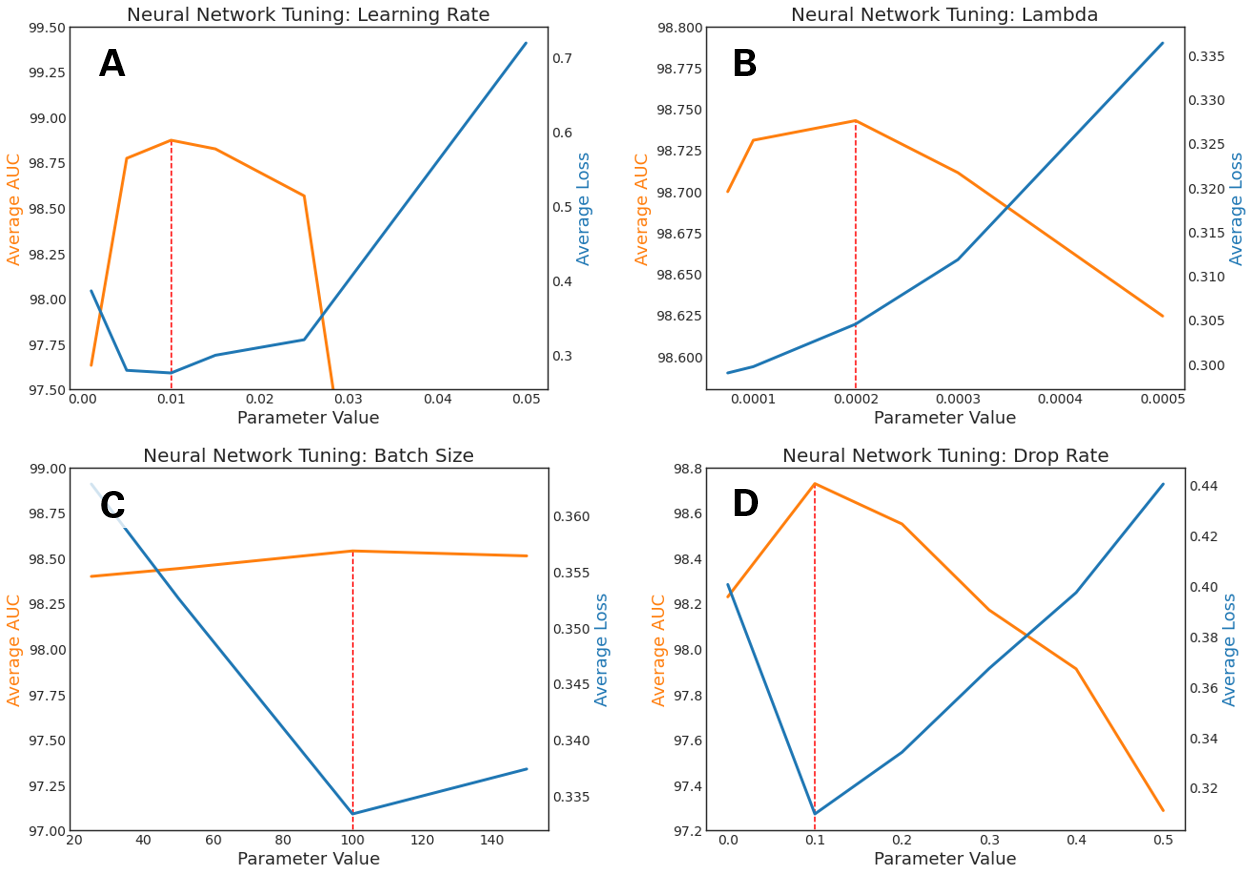
\includegraphics[width=\textwidth]{templates/images/Figure-NN_Hyperparameters.png}
\caption[Neural network hyperparameter tuning]{ANN hyperparameter tuning results for A.\ learning rate, B.\ lambda ($\lambda$), C.\ batch size, and D.\ dropout rate, using WDS4. The orange lines track AUC after 100 training epochs, averaged over 10-folds of stratified cross-validation for each hyperparameter value. The blue lines show average loss after 100 epochs. Red dashed lines mark the selected values for the final model.}
\label{fig:nn_tuning_plots}
\end{figure}

The stratified $k$-fold CV strategy described in Section \ref{ch3:strat_kfold_cv} was used for tuning ANN hyperparameters. Training continued for 100 epochs, and since TensorFlow models easily track metric values for both the training and validation sets at each epoch, the two sets were kept separate during the 10-fold CV process. In the figures and discussion that follow, results are described for WDS4. Full results for all three data sets are provided in Table \ref{tab:nn_tuning}. 

\begin{table}[htp]
\centering
\begin{tabular}{l|c|c|c|}
\cline{2-4}
                                      & \textbf{WDS}   & \textbf{WDS4}  & \textbf{WDS8}  \\ \hline
\multicolumn{1}{|l|}{\bftt{learning rate}}   & 0.005 & 0.010 & 0.010 \\ \hline
\multicolumn{1}{|l|}{\bftt{lambda ($\lambda$)}}          & 0.0001 & 0.0002 & 0.0001 \\ \hline
\multicolumn{1}{|l|}{\bftt{batch size}}      & 50    & 100   & 150   \\ \hline
\multicolumn{1}{|l|}{\bftt{dropout rate}}    & 0.3   & 0.1   & 0.1   \\ \hline
\multicolumn{1}{|l|}{\bftt{epochs}}          & 25    & 100   & 200   \\ \hline
\multicolumn{1}{|l|}{\bftt{Accuracy$_{train}$}} & 0.777 & 0.959 & 0.965 \\ \hline
\multicolumn{1}{|l|}{\bftt{Accuracy$_{test}$}}  & 0.742 & 0.949 & 0.957 \\ \hline
\multicolumn{1}{|l|}{\bftt{AUC$_{train}$}}      & 0.952 & 0.998 & 0.999 \\ \hline
\multicolumn{1}{|l|}{\bftt{AUC$_{test}$}}       & 0.863 & 0.992 & 0.992 \\ \hline
\end{tabular}
\singlespacing
\caption[Neural network hyperparameter tuning results]{ANN hyperparameter tuning results for each data set. Accuracy and AUC metrics are split into train (in-sample) and test (out-of-sample) values.}
\label{tab:nn_tuning}
\end{table}

\begin{figure}[htp]
\centering
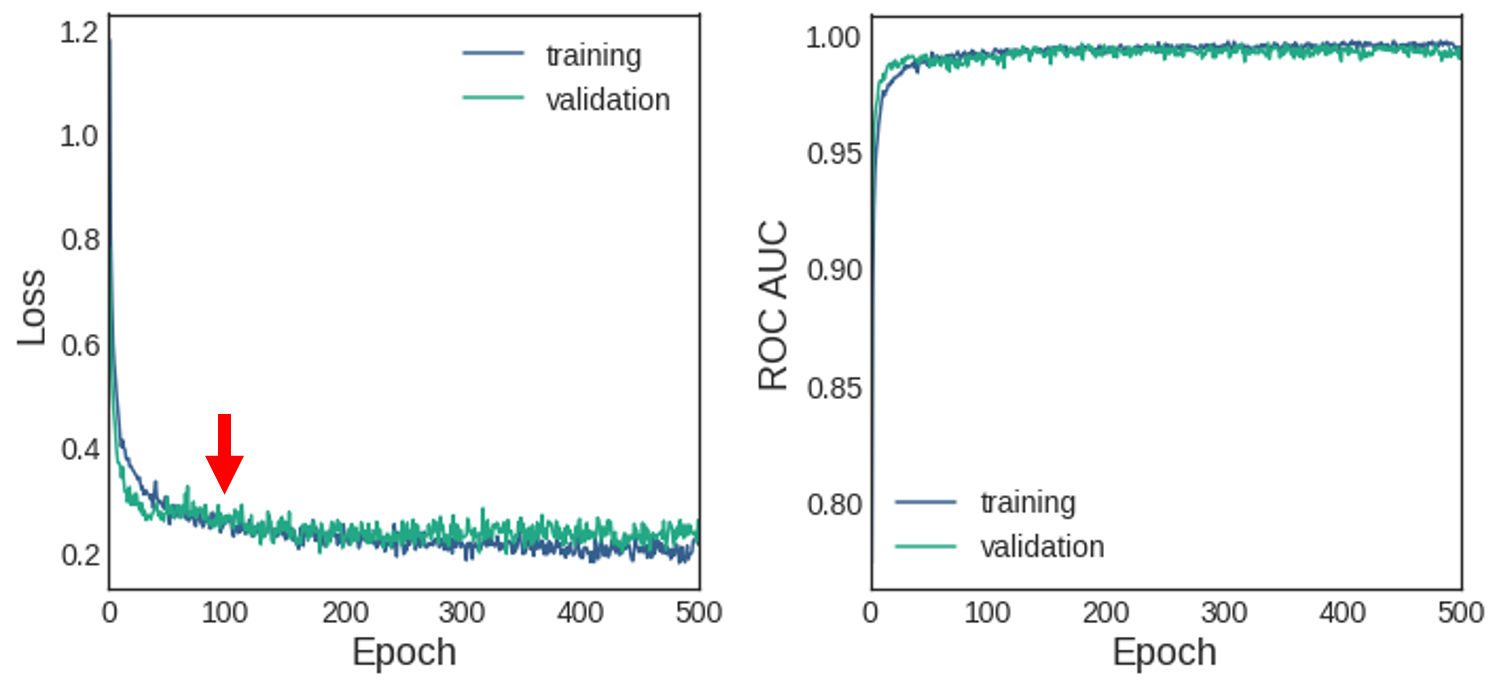
\includegraphics[width=\textwidth]{templates/images/Figure-NN-Training-Loss.png}
\caption[Neural network training loss]{ANN training results as a function of epoch count for WDS4. Calculated loss (Left) and AUC (Right) for the training (blue) and validation (green) subsets converge and start to separate near the 100-epoch mark (red arrow). Mini-batch related noise obscures the exact cross-over location.}
\label{fig:nn_loss_plot}
\end{figure}

Tuning was conducted in the same order as listed in Figure \ref{fig:nn_tuning_plots}. Distinct maxima in CV-averaged AUC are observed for each hyperparameter. The selected values for the final WDS4 model include: \verb|learning_rate| of 0.01, \verb|lambda| value of $2\times10^{-4}$, \verb|batch_size| of 100, and \verb|dropout_rate| of 0.1. Minima in the average loss curves align with the selected hyperparameter values for all except \verb|lambda|, the regularization parameter on model weights. This matches the expected behavior described in Equation \ref{eq:nn_cost_function}, where \verb|lambda| controls the balance between loss and sum of squared weights in the cost function. As Figure \ref{fig:nn_tuning_plots}B shows, the loss term decreases as \verb|lambda| approaches zero.

Figure \ref{fig:nn_loss_plot} illustrates the WDS4 training progress as a time series of loss and AUC. The variance in both plots reflects noise introduced by mini-batch training, but convergence takes place quickly. The growing separation between the training and validation loss at greater epoch counts indicates the model is overfitting the training data. The cross-over of the training and validation lines, which corresponds with the tuned value for the \verb|epoch| hyperparameter, occurs somewhere close to 100 epochs for WDS4.

\subsection{Optimized Model Results}\label{ch5:nn_final_results}

The ANN model was re-trained for each of the three data sets using the hyperparameter values listed in Table \ref{tab:nn_tuning}. Data sparsity is problematic for the WDS model; even after careful tuning, the out-of-sample accuracy does not exceed 75\%, and test set AUC is just $\approx86\%$. Models trained and tested on respective subsets of WDS4 and WDS8 demonstrate $\approx95\%$ accuracy and AUC values $>99\%$ (Table \ref{tab:nn_tuning}). Although there is the concern of added spatial correlation through the kriging approach to geothermal gradient imputation described in Section \ref{ch3:imputation}, the imputed data sets provide much-needed constraints for training the many ANN model parameters. 
 
\begin{figure}[htp]
\centering
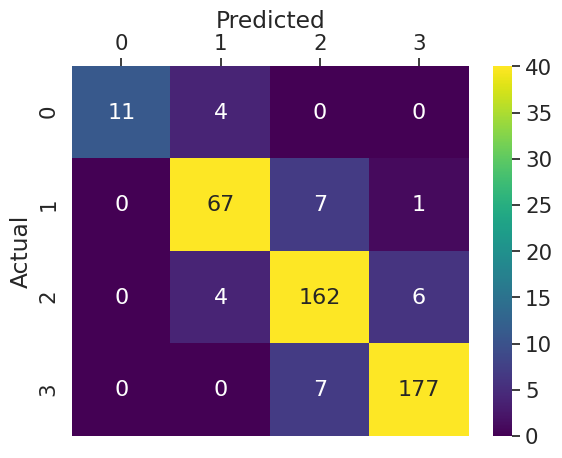
\includegraphics[width=.5\textwidth]{templates/images/Figure-NN-ConfusionMatrix_WDS4.png}
\singlespacing
\caption[Neural network confusion matrix]{Confusion matrix for the tuned ANN model trained on WDS4.}
\label{fig:nn_confusion_matrix}
\end{figure}

Figure \ref{fig:nn_confusion_matrix} depicts the confusion matrix constructed from WDS4 model results. Similar to XGBoost model performance, nearly all of the misclassifications are off by only a single sequential class assignment, the most prevalent being between medium-grade (class 2) and high-grade (class 3) geothermal gradient. Overall, these are very strong results for a predictive classifier.

Figure \ref{fig:nn_auc} shows the macro average, micro average, and individual class ANN ROC curves. All individual class AUC values are at or above 0.99, as was the case for the XGBoost model. This is close to an ideal ROC plot for a classifier.

\begin{figure}[htp]
\centering
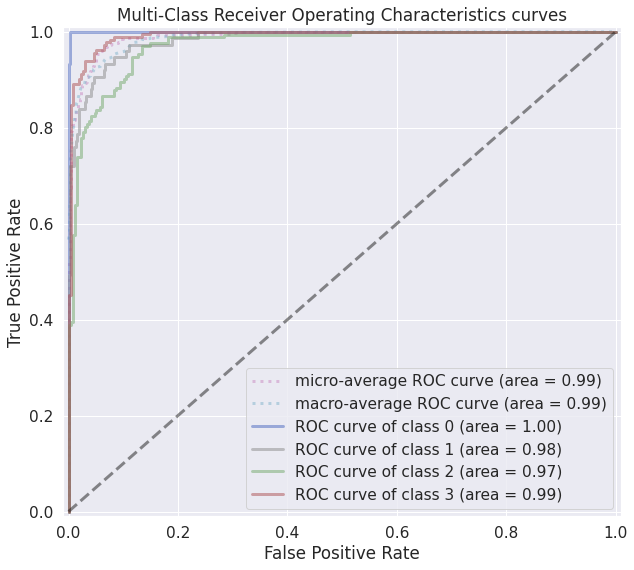
\includegraphics[width=0.7\textwidth]{templates/images/Figure-NN-AUC.png}
\caption[Neural network ROC curves]{ROC curves for tuned ANN model trained on WDS4.}
\label{fig:nn_auc}
\end{figure}

\begin{figure}[!htp]
\centering
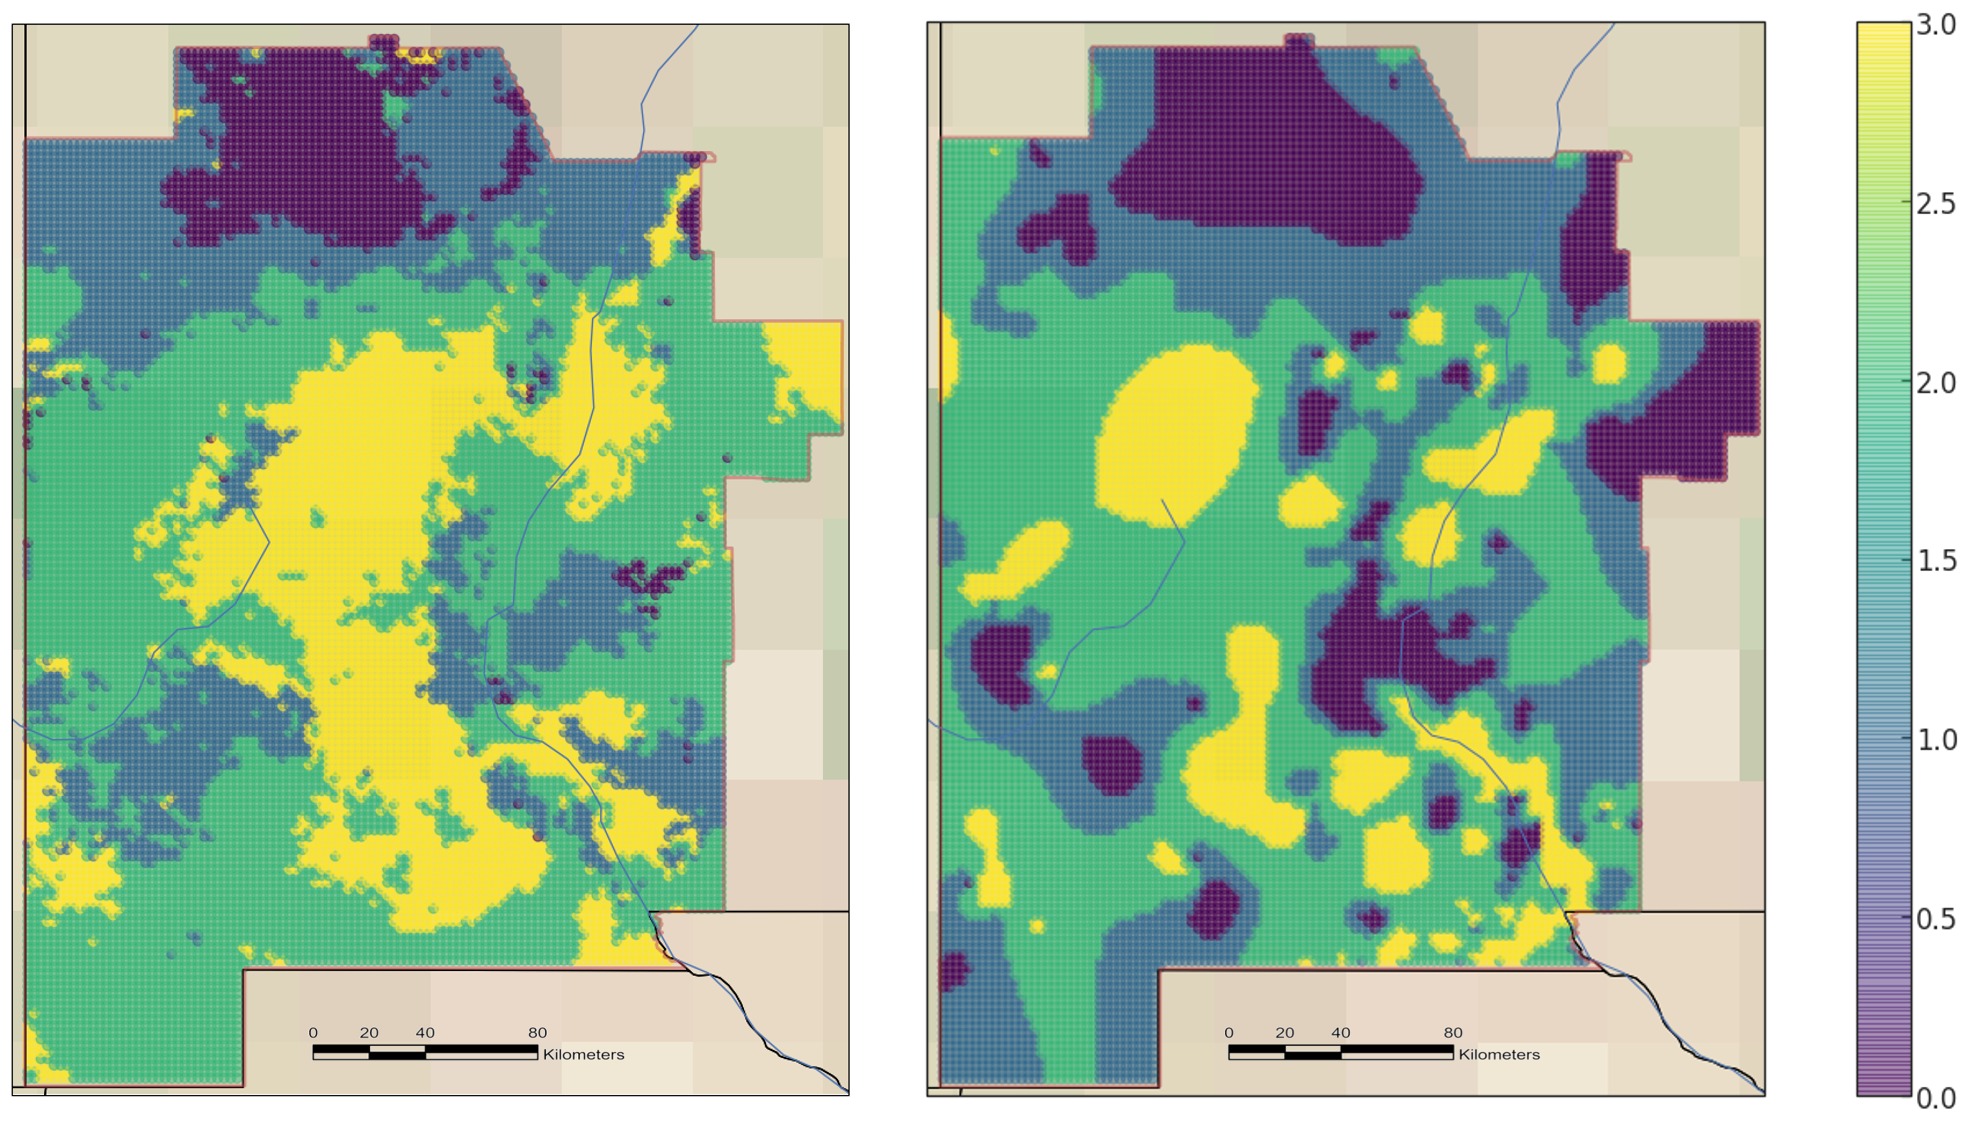
\includegraphics[width=\textwidth]{templates/images/Figure-NN-FinalMap_Joint.png}
\caption[Neural network prediction map]{Left: Map predictions of geothermal gradient from the tuned ANN model trained on WDS4. Right: geothermal gradient feature layer from Southwestern NM PFA study \protect\citep{bielicki_hydrogeolgic_2015}.}
\label{fig:nn_final_map}
\end{figure}

The FDS was passed through the final ANN model to generate predictions for the full study area, as shown in Figure \ref{fig:nn_final_map}. Class-3 high-grade geothermal-gradient regions to the southeast in the \citet{bielicki_hydrogeolgic_2015} PFA layer are well captured by the ANN model. The class-3 swath though the center of the AOI describes a broader, more continuous region of gradient potential than suggested by the PFA map. Additional high-gradient patches unique to the ANN map appear along the study-area edges –- in the southwest corner (Basin and Range), eastern panhandle (Great Plains), and to the northeast, following the Rio Grande. The low-gradient zone to the north (Colorado Plateau) matches between the two maps, but most other class-0 areas in the \citeauthor{bielicki_hydrogeolgic_2015} map are not observed in the ANN map. Interestingly, there appears to be greater overall similarity between the ANN map in Figure \ref{fig:nn_final_map} and the XGBoost map in Figure \ref{fig:xgb_final_map} than with the PFA map.

\section{Uncertainty Analysis}\label{ch5:uncertainty_analysis}

\subsection{Structural Uncertainty}\label{ch5:structural_uncertainty}

Figure \ref{fig:combined_maps} shows all four machine learning model predictions for the SW NM study area. The models differ in how individual areas are classified, as well as overall character of the predictions, suggesting each model has a signature predictive style.

\begin{figure}[!htp]
\centering
\includegraphics[width=\textwidth]{templates/images/Figure-All_Models.png}
\caption[Combined machine learning results]{Machine learning results for WDS4 using A. logistic regression, B. a decision tree, C. XGBoost, and D. an artificial neural network. Results match those already shown in Figures \ref{fig:logreg_final_map}, \ref{fig:dtree_final_map}, \ref{fig:xgb_final_map}, and \ref{fig:nn_final_map}.}
\label{fig:combined_maps}
\end{figure}

Figure \ref{fig:avg_final_map}A illustrates an ensemble average map, where each location is assigned the class with the maximum average probability across the four model predictions. Aspects of all four models in Figure \ref{fig:combined_maps} can be identified in this result, but the overall effect is a simpler model with a more spatially-conservative high-grade class-3 predictions. Also missing are many of the probably spurious high-gradient patches along the AOI boundaries and within the eastern panhandle or southern boot-heel. The \citeauthor{bielicki_hydrogeolgic_2015} gradient-feature map (Figure \ref{fig:avg_final_map}B) shows much more structure in geothermal-gradient predictions by comparison, with a pock-marked appearance typical of interpolation bulls-eye patterns.

\begin{figure}[!htp]
\centering
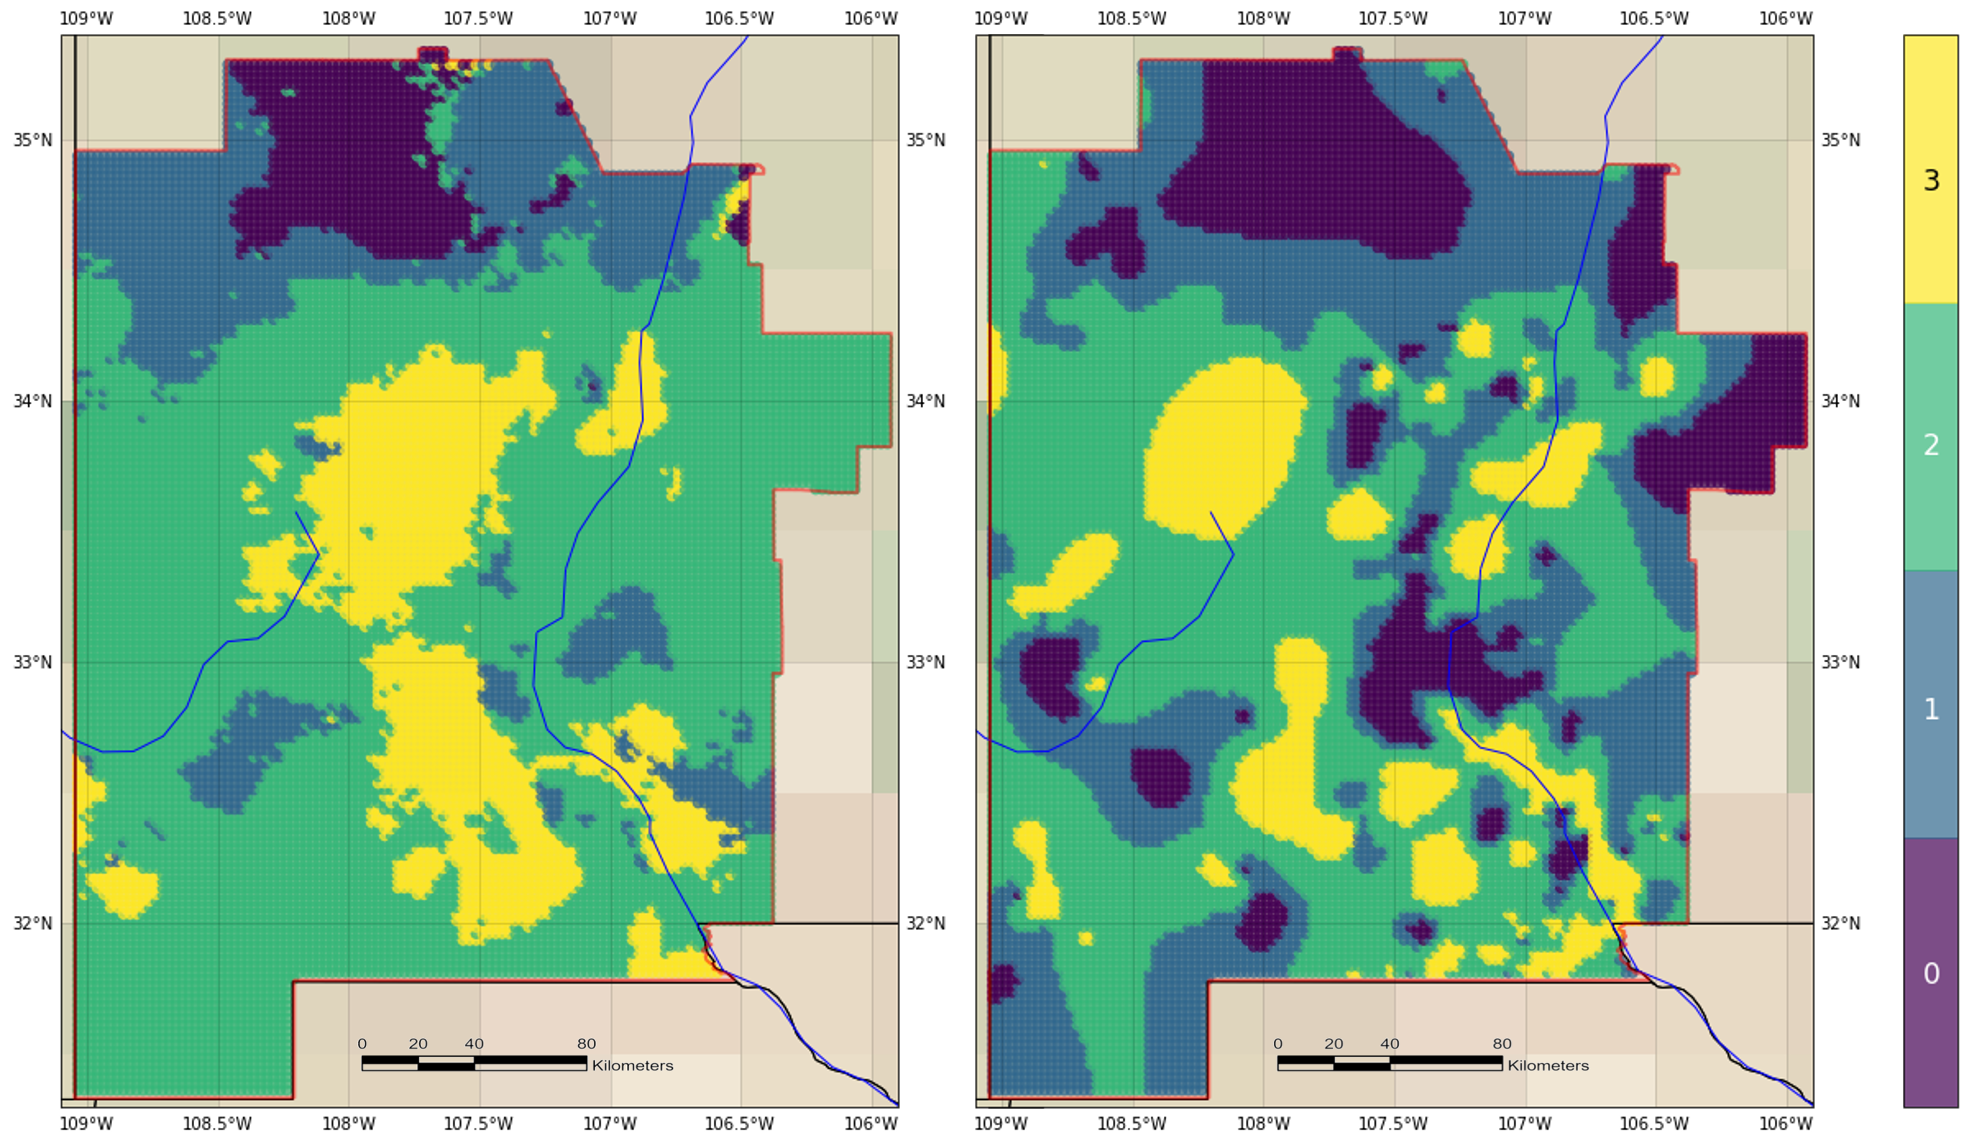
\includegraphics[width=\textwidth]{templates/images/Figure-Average_Gradient_Map_Joint.png}
\caption[Combined model prediction map]{Left: Geothermal gradient classification map from combining the four predictive models shown in Figure \ref{fig:combined_maps}. Results are for WDS4. Right: geothermal-gradient feature layer from Southwestern NM PFA study \protect\citep{bielicki_hydrogeolgic_2015}.}
\label{fig:avg_final_map}
\end{figure}

Shannon entropy is calculated on this same averaged model using the underlying class probabilities. The result is shown in Figure \ref{fig:structural_entropy_map}. Normalized entropy values vary from 0 to 1, with high entropy defining locations where there is no clear differentiation between gradient-class label probabilities. Regions colored red thus identify locations that are difficult for any model to classify, due to inconclusive feature inputs, or alternatively, locations where the predicted class probabilities from the different models varied enough that, upon averaging, they converged to similar values and could not be disentangled.

Figure \ref{fig:avg_gradient_masked_map} illustrates an alternative way of presenting these results. Regions of high entropy (> 0.7) are masked in dark gray because of the uncertainty in their classifications. All other points have a color transparency that scales with entropy. Low uncertainty/entropy areas are uncommon, focused primarily in the southwest and in small patches to the central west and central east areas. High uncertainties trace the boundaries between areas of consistent gradient classifications to the north and southeast. For example, the non-thermal region (class 0) in the Colorado Plateau to the north is ringed by high uncertainties. This highlights model inconsistencies on exactly where the class 0-class 1 boundary should appear based on trends in the input feature data.

\begin{figure}
\centering
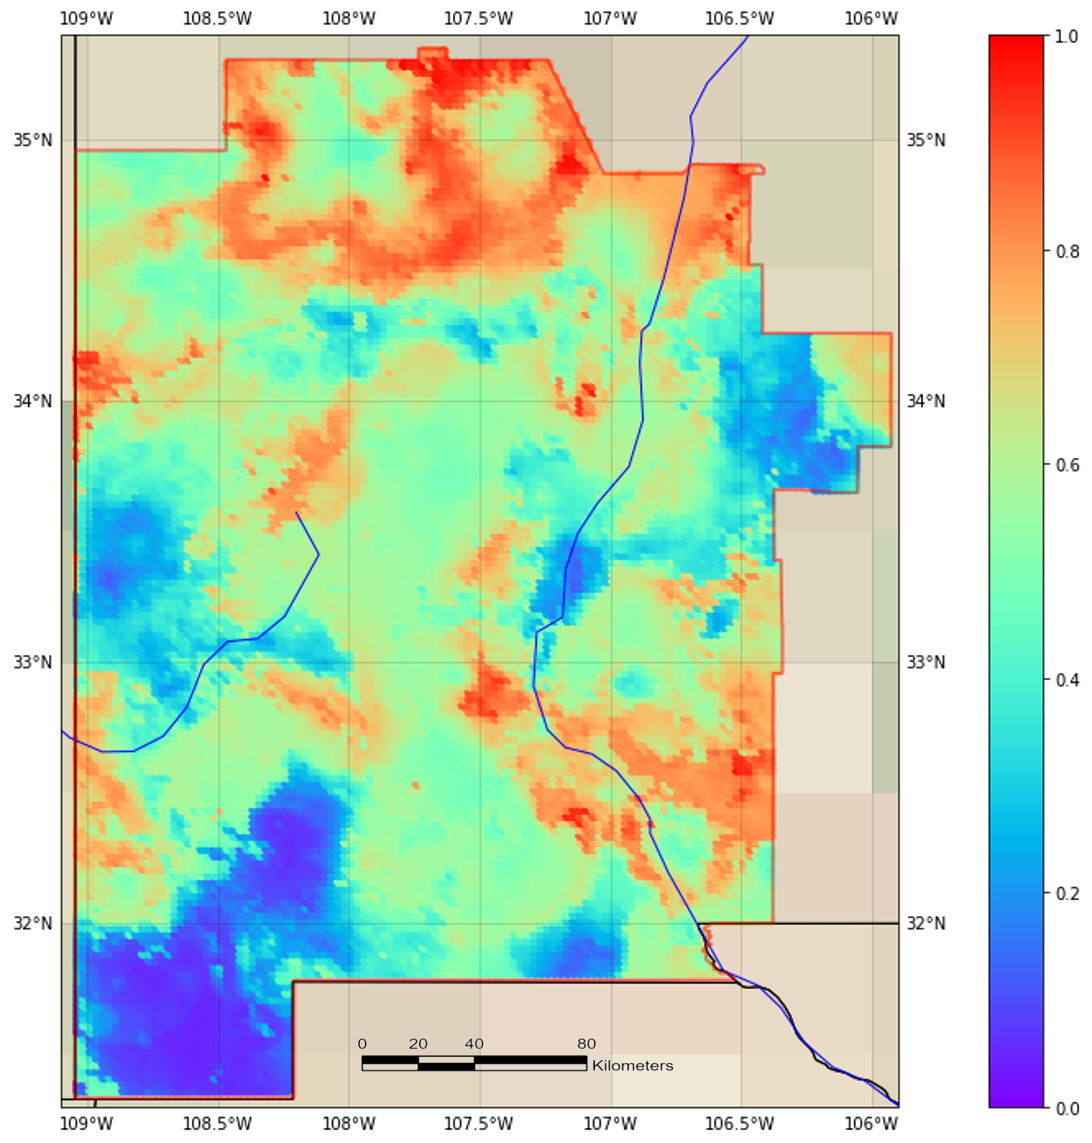
\includegraphics[width=.75\textwidth]{templates/images/Figure-Structural_Entropy_Map.png}
\caption[Structural uncertainty map]{Structural uncertainty from the choice of models, measured using Shannon entropy. Values are normalized to range from 0 for low entropy, low uncertainty (blue) to 1 for high entropy, high uncertainty (red).}
\label{fig:structural_entropy_map}
\end{figure}

\begin{figure}
\centering
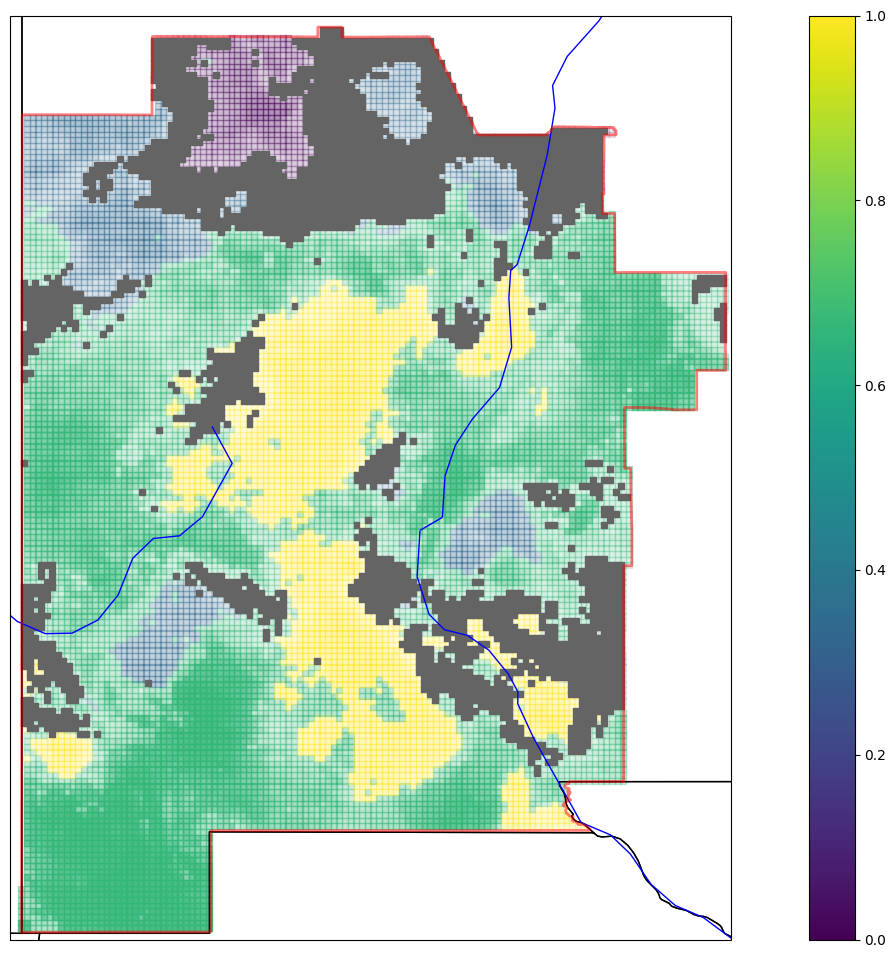
\includegraphics[width=.75\textwidth]{templates/images/Figure-Masked_Average_Gradient_Map.png}
\caption[Structural uncertainty mask on prediction map]{Combined-model prediction map with uncertainty masking. Normalized entropy values > 0.7 are grayed out and values $\leq0.7$ determine transparency of the colored scatter plot. Transparency increases from none at entropy values close to 0 to full for entropy values close to 1. The background topographic raster has been removed to better visualize the transparency effect.}
\label{fig:avg_gradient_masked_map}
\end{figure}

\subsection{Parameter Uncertainty}\label{ch5:param_uncertainty}

The TensorFlow Probability package \citep{dillon_tensorflow_2017} was used to transform the ANN from Section \ref{ch5:ann_model} into a Bayesian Neural Network (BNN) for uncertainty estimation. Given the sparsity of training data available and the multiplier effect that probabilistic layers have on the number of trainable parameters in a BNN, only the second hidden layer was converted to a TensorFlow \textit{DenseVariational} layer (Figures \ref{fig:bnn_text_structure} and \ref{fig:bnn_dot_structure}). Standard normal ($N(\mu=0, \sigma=1)$) distributions were used as priors for the layer nodes. The same tuned hyperparameter values applied to the ANN (Table \ref{tab:bnn_metrics}) were also applied to the BNN with one exception: the number of epochs was increased by a factor of 3-4. Figure \ref{fig:bnn_loss} shows the training loss and AUC curves for WDS4, which justify this larger number of epochs for training. Table \ref{tab:bnn_metrics} notes the accuracy and AUC scores for the BNNs calculated from a single predictive run on the respective test data subsets.

\begin{figure}[!htp]
\centering
\begin{minipage}[b][][b]{.35\linewidth}
    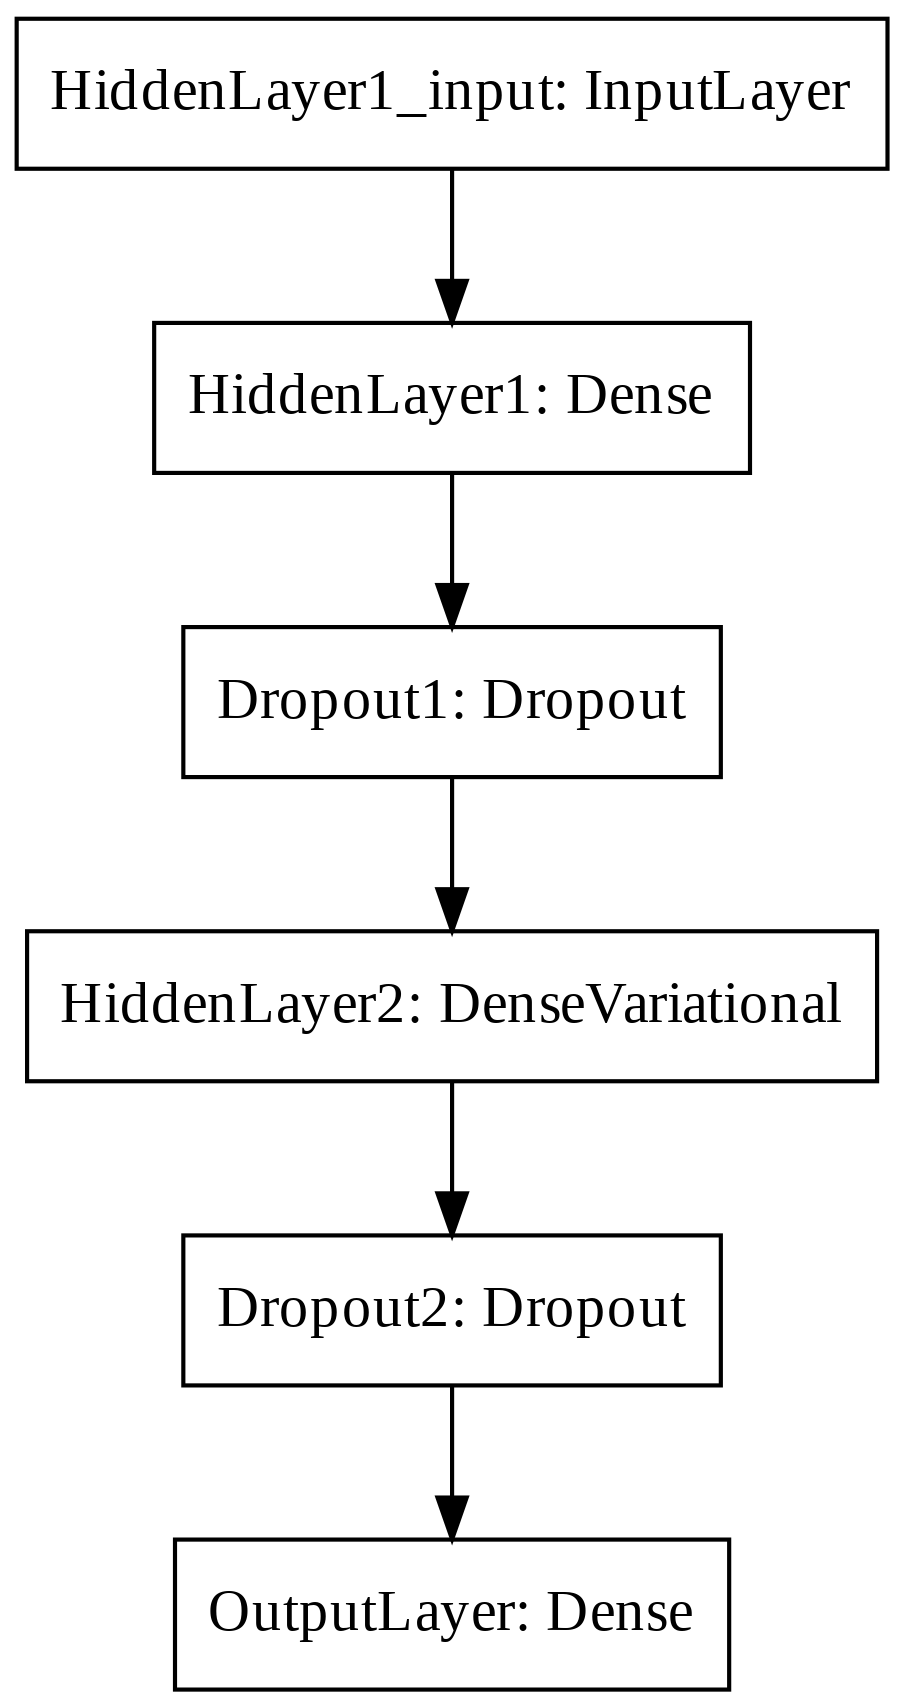
\includegraphics[width=\linewidth]{templates/images/Figure-TF_BNN_Structure.png}
    \caption[Bayesian neural network structural flow]{Structural flow chart for the Bayesian neural networks.}
    \label{fig:bnn_text_structure}
\end{minipage}
\hfill
\begin{minipage}[b][][b]{.61\linewidth}
    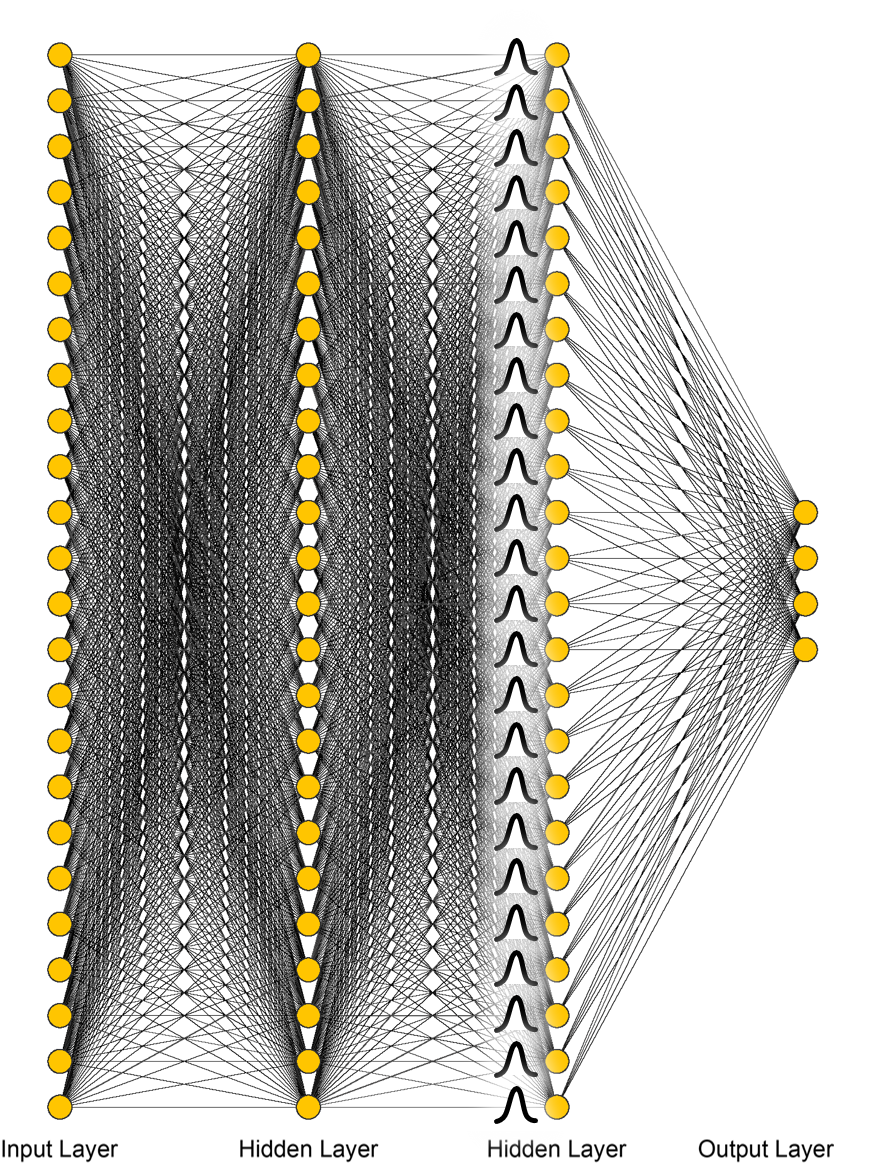
\includegraphics[width=\linewidth]{templates/images/Figure-BNN.png}
    \caption[Bayesian neural network structural schematic]{Schematic diagram of the Bayesian neural networks. Not shown are the dropout operations after each hidden layer.}
    \label{fig:bnn_dot_structure}
\end{minipage}
\end{figure}

\begin{table}[htp]
\centering
\begin{tabular}{l|c|c|c|}
\cline{2-4}
                                      & \textbf{WDS}   & \textbf{WDS4}  & \textbf{WDS8}  \\ \hline
\multicolumn{1}{|l|}{\bftt{learning rate}}   & 0.005 & 0.010 & 0.010 \\ \hline
\multicolumn{1}{|l|}{\bftt{lambda ($\lambda$)}} & 0.0001 & 0.0002 & 0.0001 \\ \hline
\multicolumn{1}{|l|}{\bftt{batch size}}      & 50    & 100   & 150   \\ \hline
\multicolumn{1}{|l|}{\bftt{dropout rate}}    & 0.3   & 0.1   & 0.1   \\ \hline
\multicolumn{1}{|l|}{\bftt{epochs}}          & 100   & 300   & 600   \\ \hline
\multicolumn{1}{|l|}{\bftt{Accuracy$_{train}$}} & 0.516 & 0.867 & 0.902 \\ \hline
\multicolumn{1}{|l|}{\bftt{Accuracy$_{test}$}}  & 0.483 & 0.869 & 0.894 \\ \hline
\multicolumn{1}{|l|}{\bftt{AUC$_{train}$}}      & 0.798 & 0.976 & 0.990 \\ \hline
\multicolumn{1}{|l|}{\bftt{AUC$_{test}$}}       & 0.762 & 0.961 & 0.980 \\ \hline
\end{tabular}
\singlespacing
\caption[Bayesian neural network hyperparameters and single-run metrics]{BNN hyperparameters and results for each data set. Accuracy and AUC metrics are split into train (in-sample) and test (out-of-sample) values. Results reflect a single prediction from the BNNs and will vary due to the stochastic nature of the feed-forward BNN operation.}
\label{tab:bnn_metrics}
\end{table}

\begin{figure}
\centering
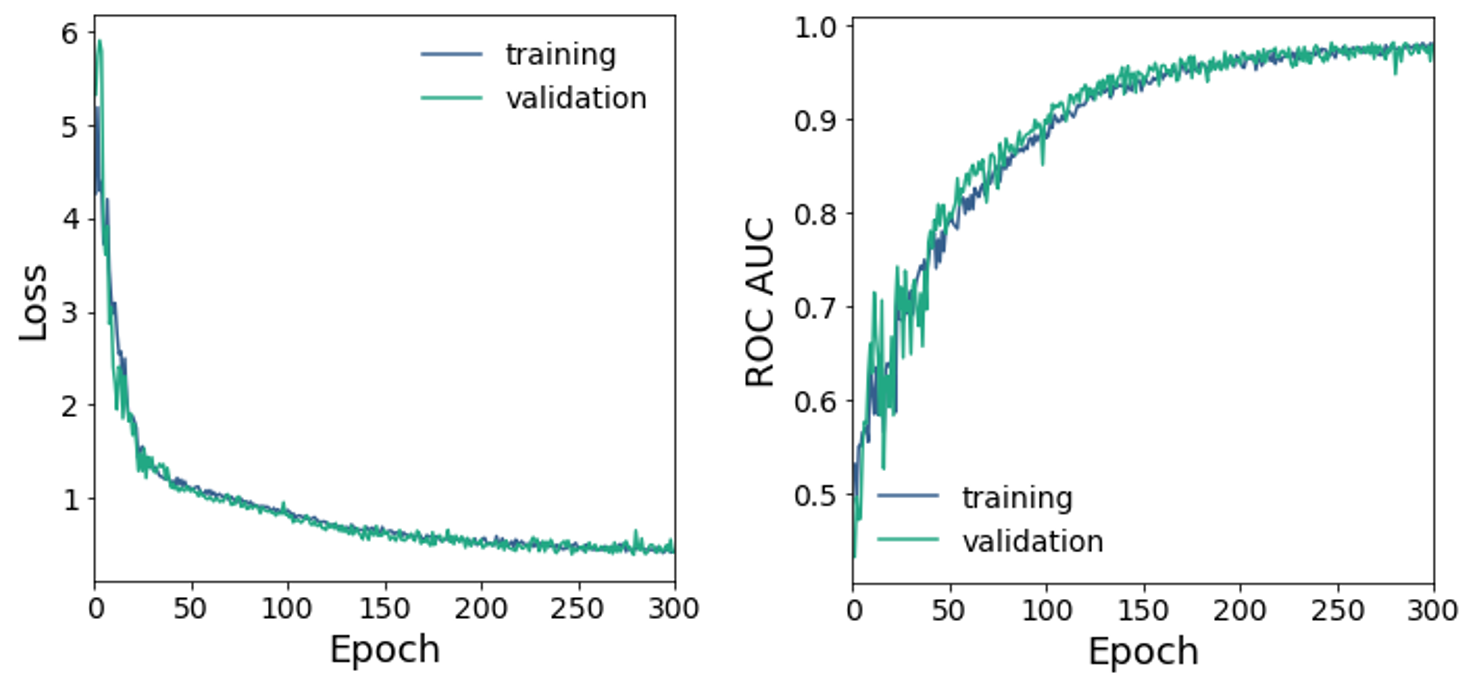
\includegraphics[width=\textwidth]{templates/images/Figure-BNN_Loss_AUC_WDS4.png}
\caption[Bayesian neural network training loss]{BNN training results as a function of epoch count for WDS4. Calculated loss (Left) and AUC (Right) for the training (blue) and validation (green) subsets show training convergence by $\approx 300$ epochs. The stochastic nature of the BNN makes the AUC/epoch curve noisier than for the deterministic ANN (Figure \ref{fig:nn_loss_plot})}
\label{fig:bnn_loss}
\end{figure}

Running the BNN multiple times will produce a collection of different model solutions. Figure \ref{fig:bnn_class_pdfs} shows the range of class label probabilities after predicting the classification of three well records 100 times using a BNN trained on the WDS4 training subset. Here, the relationship between entropy values and the overlap in class-label probabilities is apparent. A low-entropy scenario (Figure \ref{fig:bnn_class_pdfs}A) has strong stand-out between the maximum-probability class label and others, while high-entropy situations (Figure \ref{fig:bnn_class_pdfs}C) have less certainty on the class-label assignment.

\begin{figure}
\centering
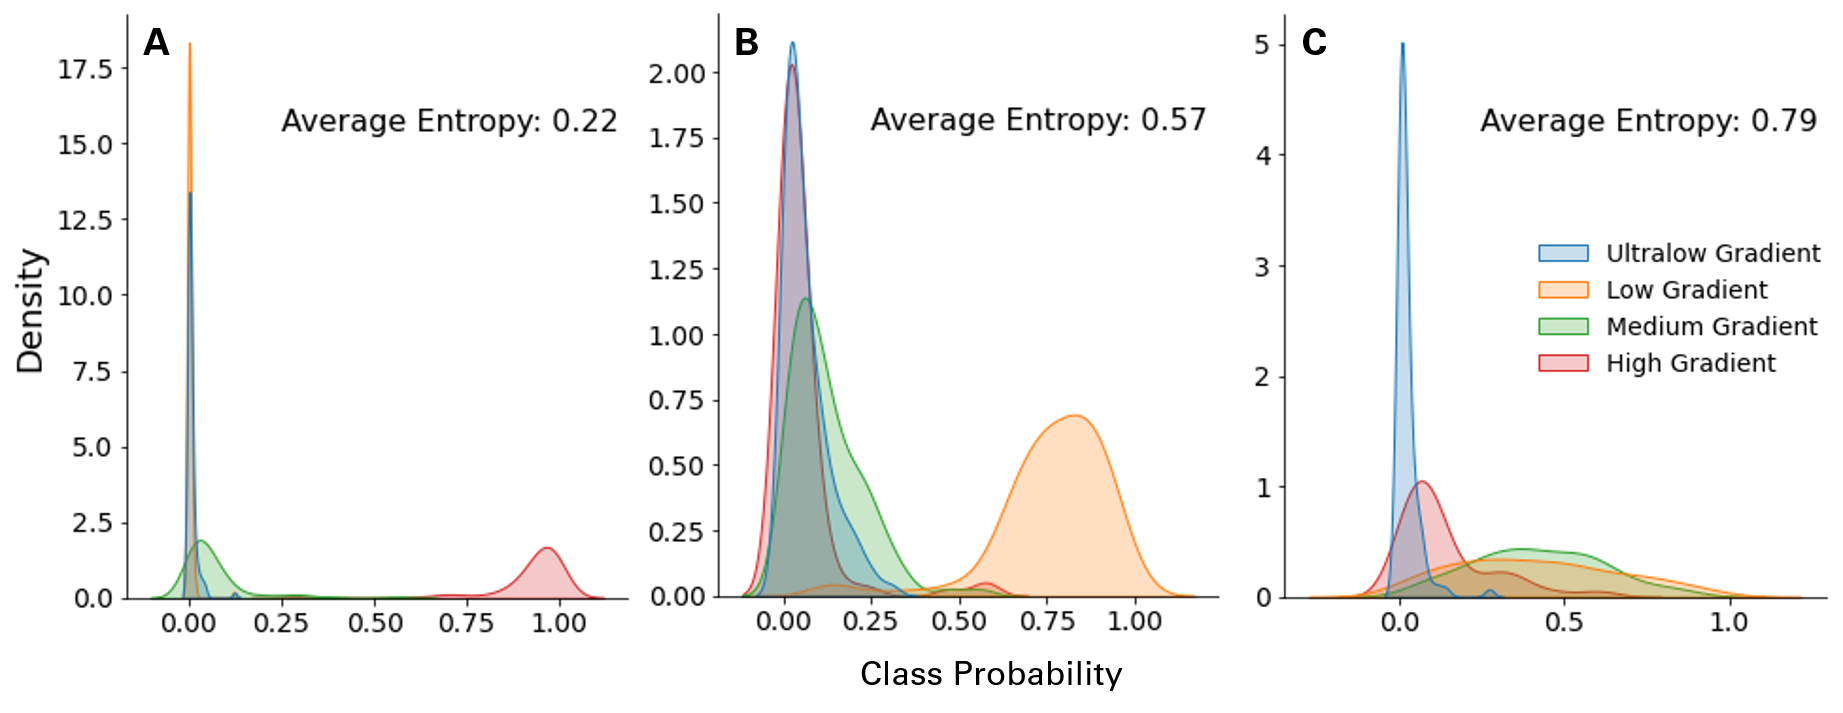
\includegraphics[width=\textwidth]{templates/images/Figure-BNN_100trials_WDS4.png}
\caption[Bayesian neural network class PDFs]{Example class label probability density functions for A.\ well record 34, B.\ well record 20, and C.\ well record 35 from WDS4. Distributions are constructed from 100 passes through the WDS4 BNN. Entropy values scale with label distribution entanglement. The predicted label is the one with the highest mean probability: A.\ High gradient, B.\ Low gradient, C.\ Medium gradient.}
\label{fig:bnn_class_pdfs}
\end{figure}

After re-training the BNN on the full WDS4 data set, predictions for the entire AOI were generated 1000 times. Geothermal-gradient class probabilities from these realizations were averaged by class for each point location, and the maximum probability class was selected as the predicted label. Entropy values calculated from the ensemble-averaged probabilities are shown in Figure \ref{fig:bnn_entropy_map}. Figure \ref{fig:bnn_masked_pred_map} combines the 1000-run average prediction map with parameter uncertainties using a layer mask and transparency. Concentrated areas of high entropy/uncertainty appear to the southeast to either side of the Rio Grande, and to the north near the edge of the Colorado Plateau (Figure \ref{fig:bnn_masked_pred_map}). Overall, there appear to be fewer locations with high entropy in the parameter uncertainty assessment compared to the structural uncertainty analysis for the four model architectures (Figure \ref{fig:avg_gradient_masked_map}).

\begin{figure}
\centering
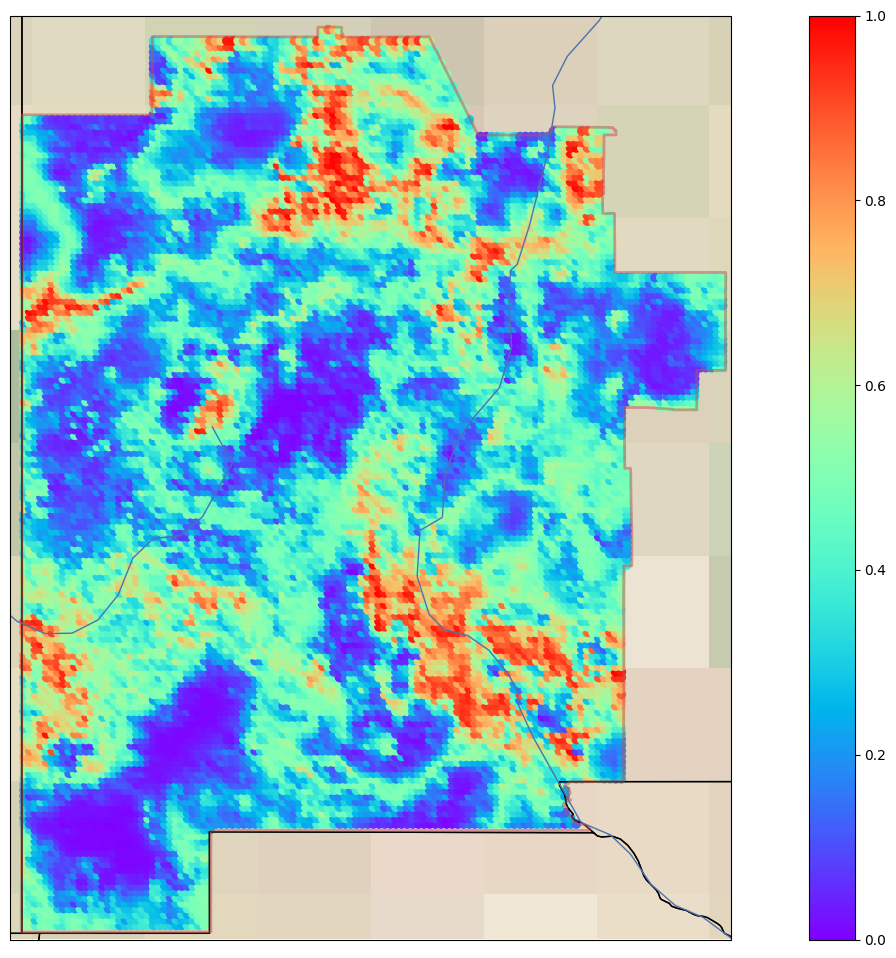
\includegraphics[width=.75\textwidth]{templates/images/Figure-BNN_Entropy_Map.png}
\caption[Bayesian neural network parameter uncertainty map]
{BNN parameter uncertainty determined from class probability averages after 1000 runs of the WDS4 predictive model. Uncertainty is measured with normalized Shannon entropy values ranging from 0 for low entropy, low uncertainty (blue) to 1 for high entropy, high uncertainty (red).}
\label{fig:bnn_entropy_map}
\end{figure}

\begin{figure}
\centering
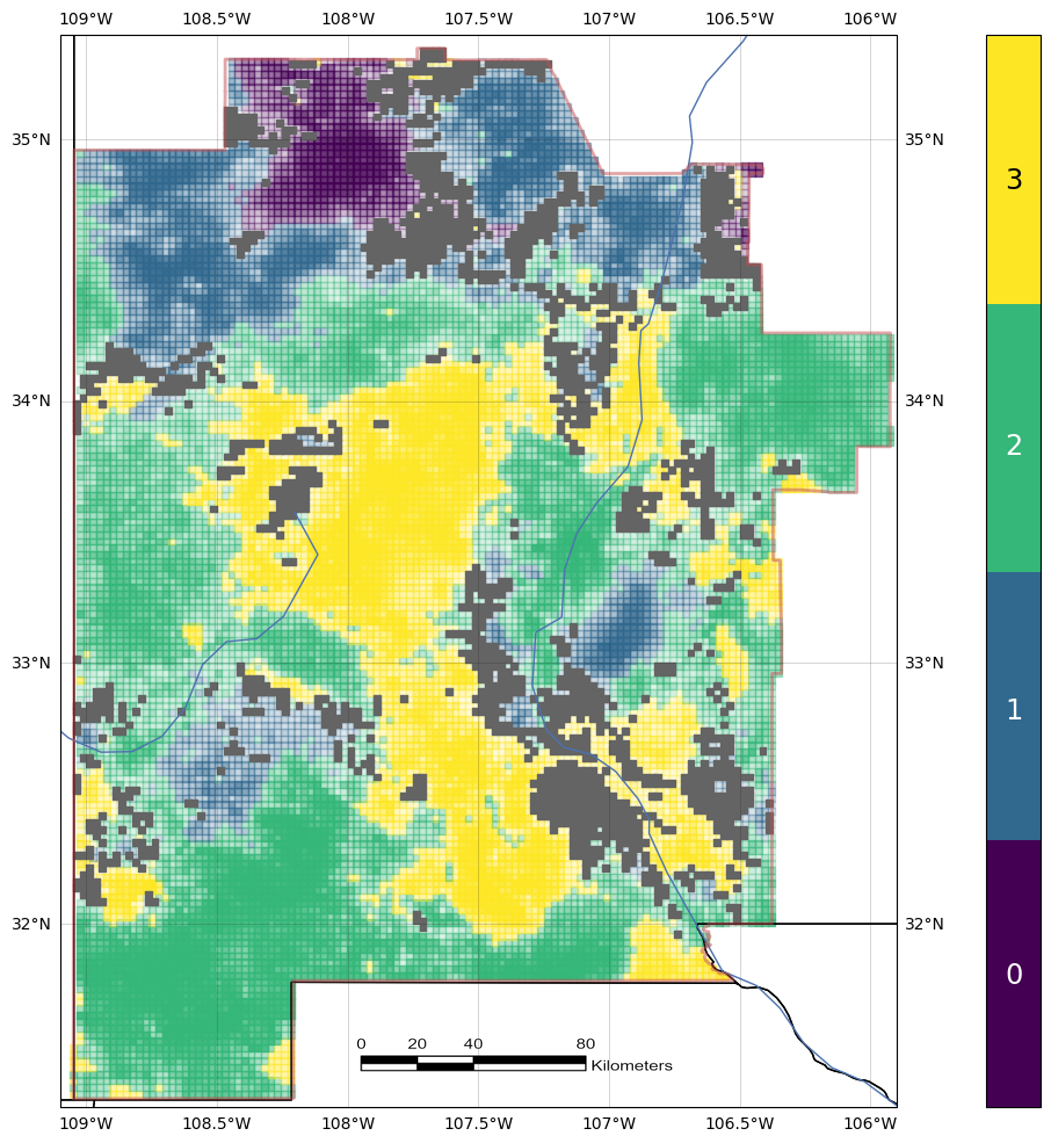
\includegraphics[width=.75\textwidth]{templates/images/Figure-BNN_All_Gradient_Map_Masked_whitebackground.png}
\caption[Parameter uncertainty mask on prediction map]
{Ensemble-averaged WDS4 BNN prediction map with uncertainty masking. Normalized entropy values > 0.7 are grayed out, values $\leq0.7$ determine transparency of the colored scatter plot. Transparency increases from none at entropy values close to 0 to full for entropy values close to 1. The background topographic raster has been removed to better visualize the transparency effect.}
\label{fig:bnn_masked_pred_map}
\end{figure}

\subsection{Measurement Uncertainty}\label{ch5:measure_uncertainty}

In the present study, the sources of data, types of data, and options for error estimation vary greatly. Several features were acquired as pre-gridded raster files without accompanying error assessments or access to the original source data (Table \ref{tab:features}), e.g., air temperature, precipitation, strain rate, and layers from the \citeauthor{bielicki_hydrogeolgic_2015} OpenEI submission \citep{kelley_geothermal_2015}. Table \ref{tab:feature_std_error} shows the top ten features identified by Shapley analysis for the XGBoost model in Section \ref{ch5:xgb_feature_selection}. Among those variables, \acrlong{sigt} (\acrshort{sigt}), Heat Flow, and Boron Concentration have readily-available standard error estimates either from the original source or data preparation process. Crustal Thickness standard error is both unknown and difficult to ascertain; the feature grid comes from contours fit to 2-D seismic models \citep{keller_comparative_1991}, which are unavailable for further analysis. The remaining top-ten features consist of point or line data converted to density layers using KDE. Standard errors could be estimated for these features by performing bootstrap or jackknife resampling, applying KDE on the derived data sets, and calculating standard errors from that sample population \multicitep{james_introduction_2013, p.\ 187--190;mcintosh_jackknife_2016}.

\begin{table}[htp]
\centering
\resizebox{\textwidth}{!}{
\begin{tabular}{|c|c|c|p{7cm}|}
\hline
\textbf{Name}                     & \textbf{Type}         & \textbf{Std Err Estimation} & \multicolumn{1}{c|}{\textbf{Comments}}             \\ \hline
Si-Geotherm.\ Temperature & Overlapping points & Kriging & Standard error estimates directly from kriging. \\ \hline
Heat Flow & Non-overlapping points & Directly provided & Standard error estimates provided for each grid point. \\ \hline
Crustal Thickness & Lines & Unknown & Contours based on 2-D seismic lines. Uncertainty in interpretation   (e.g., velocity model) unavailable. \\ \hline
Volcanic Dike Density & Lines & Resampling & Jackknife/bootstrap resample and generate density estimates. \\ \hline
Spring Density & Non-overlapping points & Resampling & Jackknife/bootstrap resample and generate density estimates. \\ \hline
Earthquake Density & Overlapping Points & Resampling & Jackknife/bootstrap resample and generate density estimates. \\ \hline
Volcanic Vent Density & Non-overlapping points & Resampling & Jackknife/bootstrap resample and generate density estimates. \\ \hline
Boron Concentration & Overlapping points & Kriging & Standard error estimates directly from kriging. \\ \hline
Quaternary Fault Density & Lines & Resampling & Jackknife/bootstrap resample and generate density estimates. \\ \hline
Drainage Density & Lines & Resampling & If extracted from DEM, relates to DEM slope error. However, can probably use jackknife/bootstrap method. \\ \hline
\end{tabular}}
\caption[Feature standard error estimation]{Methods of determining standard error estimates for the top ten most important features, identified from Shapley analysis of the WDS4 XGBoost classifier (see Figure \ref{fig:xgb_shap_global}).}
\label{tab:feature_std_error}
\end{table}

Shapley results show that SiGT values influence the XGBoost model predictions more than any other feature (Figure \ref{fig:xgb_shap_global}). Uncertainty in the values for this feature should therefore translate into uncertainty in the classification results. To examine this relationship further, the SiGT values assigned to well locations in WDS4 were perturbed to create a range of statistically-similar derived data sets. Variability in the classification results after training on these data sets highlights model sensitivity to uncertainties in the feature measurements.

\begin{figure}
\centering
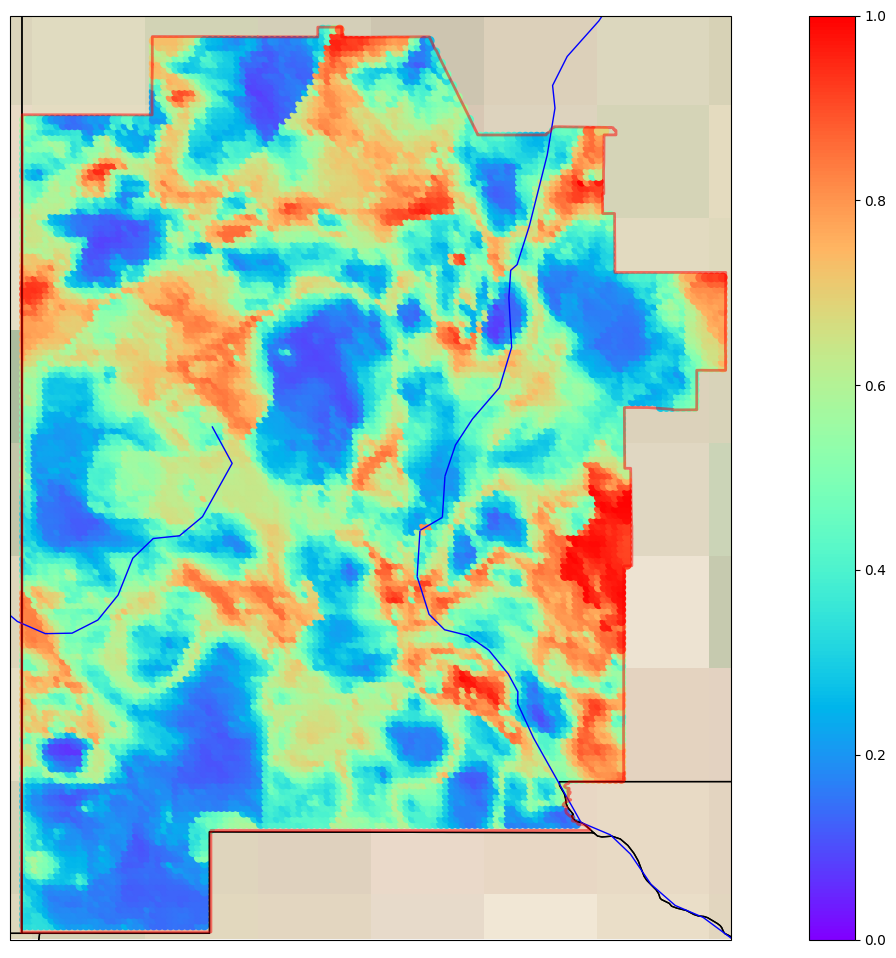
\includegraphics[width=.75\textwidth]{templates/images/Figure-MU_Entropy_Map.png}
\caption[SiGT measurement uncertainty map]
{SiGT measurement uncertainty based on normalized Shannon entropy. Calculations were made on class probability averages after modeling 100 randomly-perturbed realizations with the WDS4 XGBoost classifier. Values range from 0 for low entropy, low uncertainty (blue) to 1 for high entropy, high uncertainty (red).}
\label{fig:mu_entropy_map}
\end{figure}

A SiGT standard error estimate map (Figure \ref{fig:mu_stderr_entropy}A) was derived using the ArcGIS \textit{Empirical Bayes Kriging} method as described in Section \ref{ch3:ebk}. All SiGT observations were included in the algorithm, so variability in coincident points due to repeated field measurements influences the estimate. Standard errors were sampled from this map at WDS4 well locations and used to construct a normal distribution ($N(0,\sigma)$) for each location. A total of 100 variants of WDS4 were created by applying perturbations to the WDS4 SiGT values sampled from these distributions. 

\begin{figure}
\centering
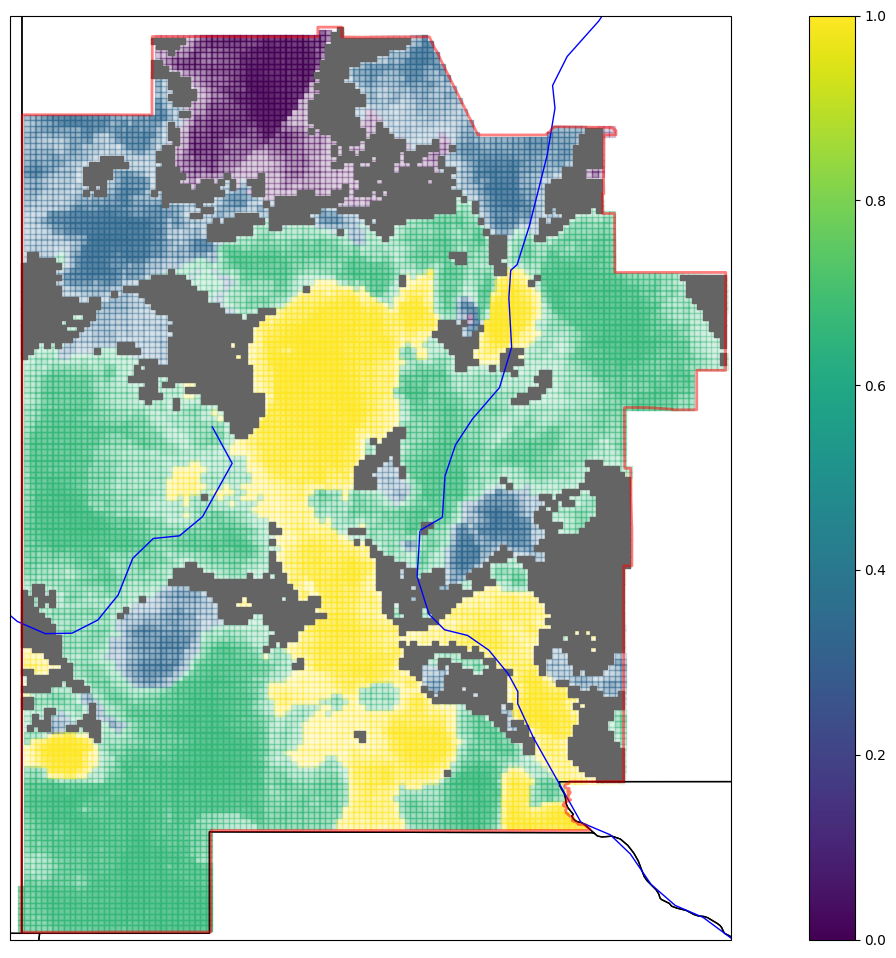
\includegraphics[width=.75\textwidth]{templates/images/Figure-MU_Masked_Average_Gradient_Map.png}
\caption[SiGT measurement uncertainty mask on prediction map]
{Ensemble-averaged WDS4 XGBoost prediction map with SiGT measurement uncertainty masking. Normalized entropy values (> 0.7) are grayed out, and values $\leq0.7$ determine transparency of the colored scatter plot. Transparency increases from none at entropy values close to 0, to full for entropy values close to 1. The background raster has been removed to better visualize the transparency effect.}
\label{fig:mu_masked_pred_map}
\end{figure}

XGBoost models, parameterized as described for WDS4 in Table \ref{tab:xgb_tuning}, were trained on the perturbed data sets and used to predict geothermal gradient classifications for the FDS covering the full AOI. After ensemble-averaging the class probabilities at each point, the maximum probability class was selected as the class assignment for the average geothermal-gradient classification map. Shannon entropy values calculated from the average class probabilities are shown in Figure \ref{fig:mu_entropy_map}. Figure \ref{fig:mu_masked_pred_map} combines both maps using entropy values > 0.7 as a layer mask and assigning increasing transparency with greater entropy for the remaining points.

\begin{figure}[!htp]
\centering
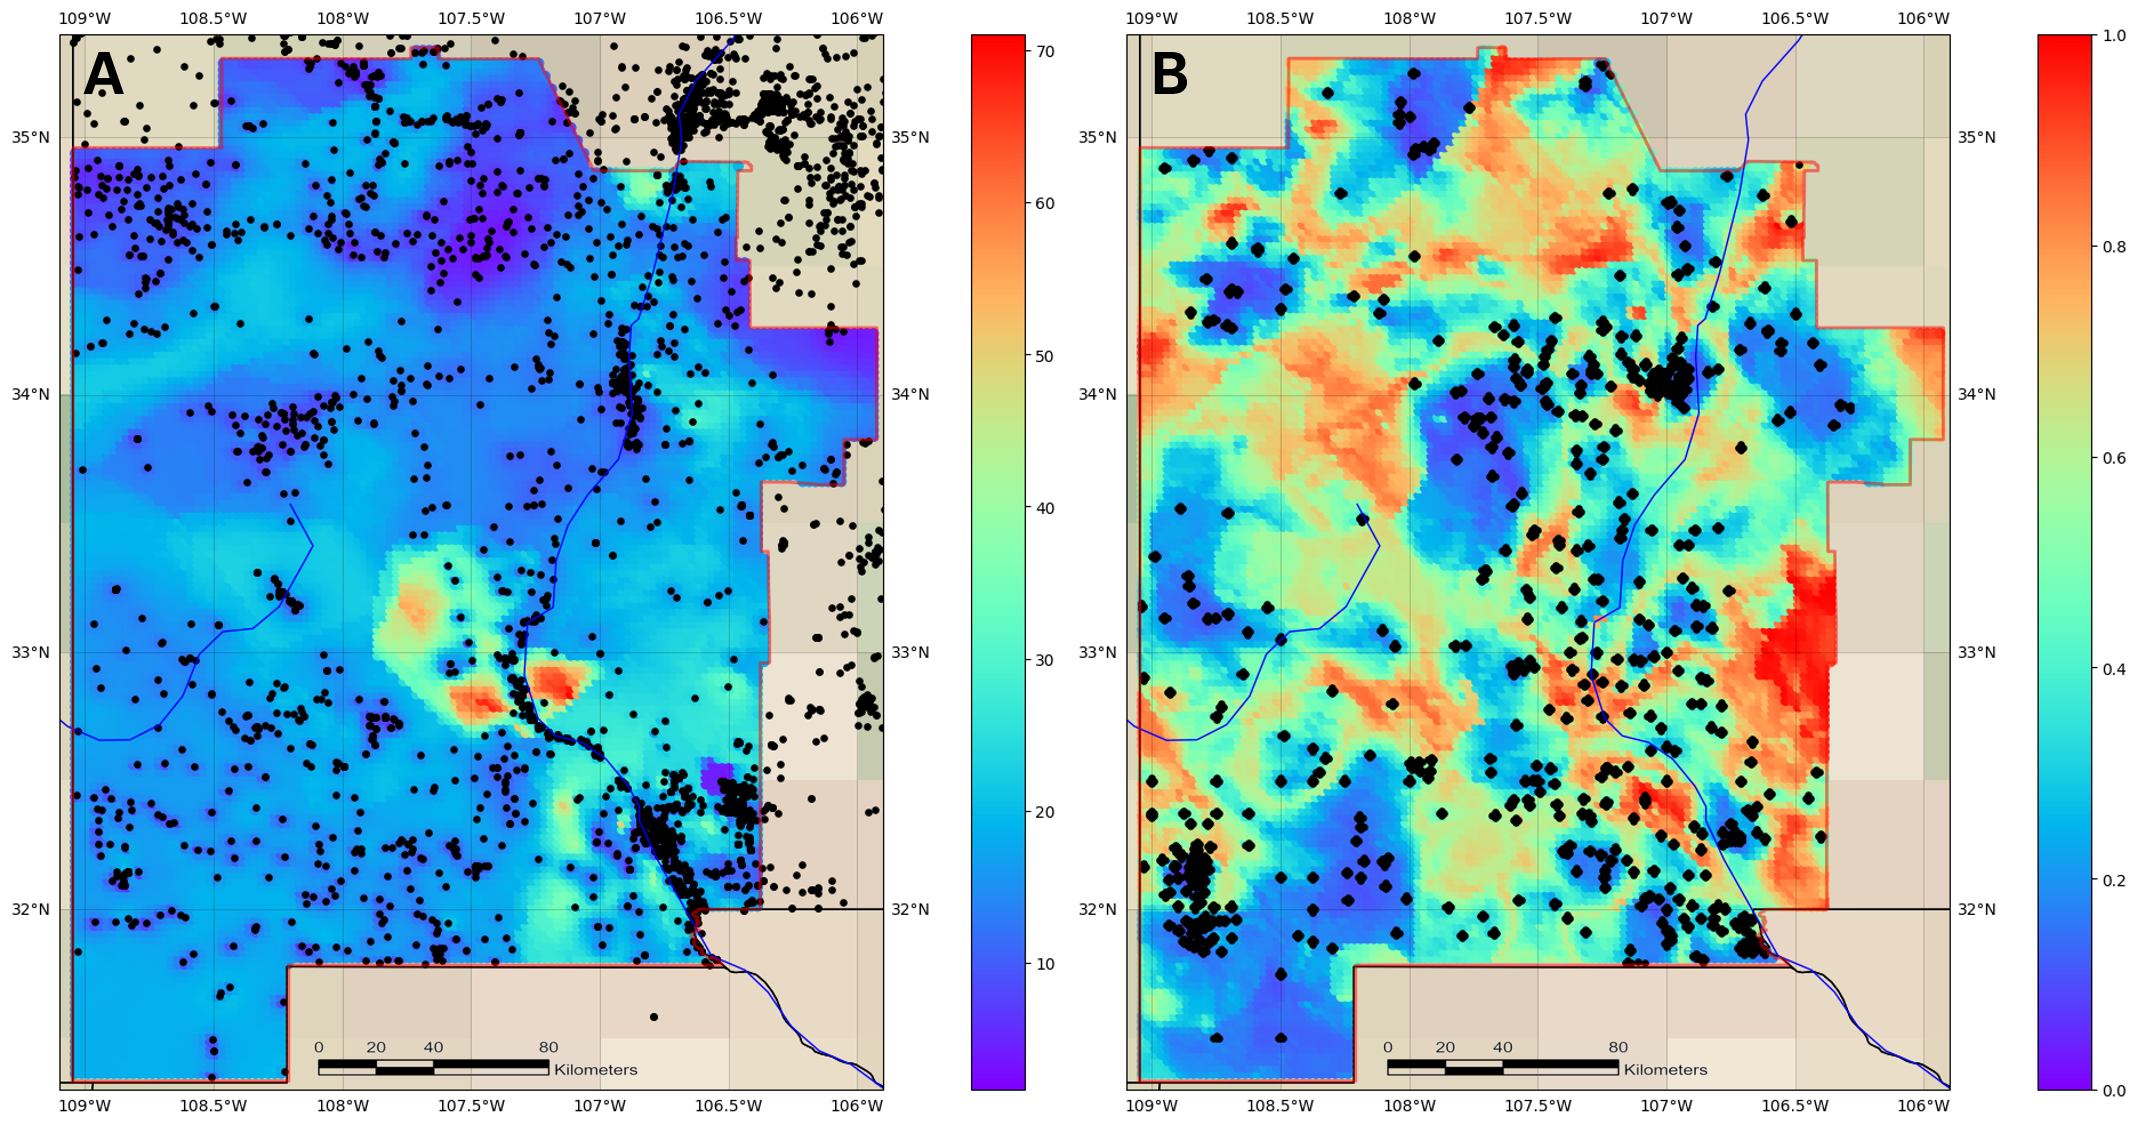
\includegraphics[width=\textwidth]{templates/images/Figure-MU_StdErr_vs_Uncert.png}
\caption[SiGT standard error and model entropy]
{A.\ SiGT standard-error map derived from kriging operation in ArcGIS. Block dots show the locations of the silica concentration samples that are the feature source data. B.\ WGS4 XGBoost measurement-uncertainty entropy map. Black circles indicate well locations in WDS4 used for training the final XGBoost classifier. }
\label{fig:mu_stderr_entropy}
\end{figure}

Interestingly, variations in SiGT values result in high classification uncertainty in many locations across the AOI (Figure \ref{fig:mu_masked_pred_map}). Concentrated areas of uncertainty are observed in the east-southeast ---an area where silica samples were collected but not where many WDS4 well observations are located (Figure \ref{fig:mu_stderr_entropy}A-B). Similarly, large patches of higher entropy appear in the north and just west of the AOI center. These are also under-sampled regions in WDS4 (Figure \ref{fig:mu_stderr_entropy}B). It appears that as training data values for SiGT change due to perturbations, thresholds for XGBoost decision trees shift enough to significantly impact the stability of model predictions away from wells. SiGT-related splits will appear near the root node of decision trees based the dominance of SiGT over other features for classification importance. Changes to the decision thresholds will thus have a strong cascading effect on the final classification choices for XGBoost models. The problem lies in both the magnitude of SiGT standard errors as well as the heterogeneous sampling of the study area by WDS4 well locations. The degree of uncertainty seen here would likely be reduced if WDS4 had more comprehensive coverage of the study area.

\section{Comparative Study Insights}\label{ch5:case_insights}

\subsection{Southwestern New Mexico PFA}\label{ch5:caase_nm_pfa}

In the Southwestern NM PFA project, \citet{bielicki_hydrogeolgic_2015} focused on hydrogeologic windows, defined as areas where erosion, faulting, or volcanic intrusions breach regional sealing layers and allow heated groundwater to reach the surface. Fundamentally, their work targeted hydrothermal systems when assigning geothermal favorability scores, treating heat, fluid volume, and flow path/reservoir as the key risk elements. The last risk element combines particle tracking of geochemical signatures (lithium, boron) with fluid recharge-discharge pathways, effectively replacing permeability and seal risk elements with a model of the subsurface water cycle. Although interesting in its own right, the integrated nature of the PFA favorability map makes it a poor benchmark for the machine-learning results here which focus on the heat-risk element alone. Instead, the geothermal-gradient feature map described in Figure \ref{app:dl_geothermal_gradient}, which \citet{bielicki_hydrogeolgic_2015} derived from NGDS data paired with additional oil \& gas well measurements, serves as the best reference for comparison. 

\begin{figure}
\centering
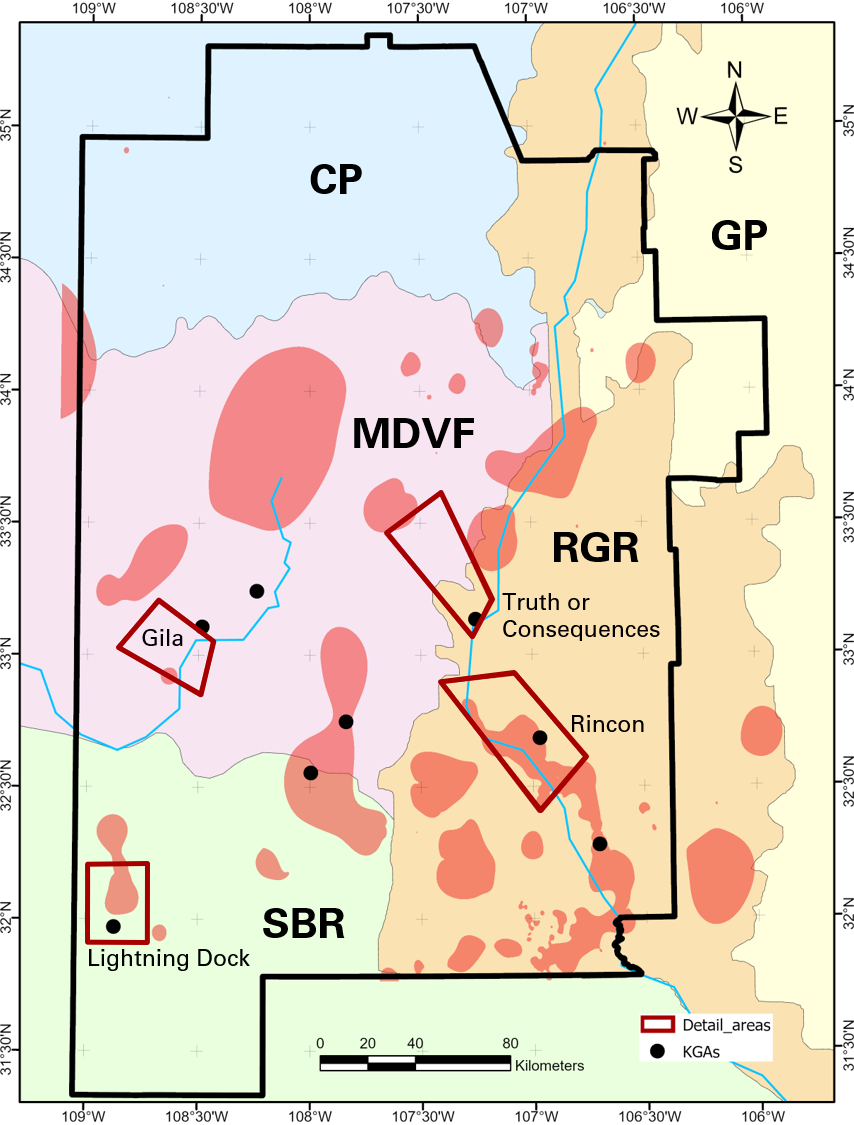
\includegraphics[width=.75\textwidth]{templates/images/Figure-PFA_Gradient_Labels.png}
\caption[SW New Mexico PFA prospective areas]
{Four prospective areas (dark red quadrangles) selected among several in the Southwestern NM PFA study \protect\citep{bielicki_hydrogeolgic_2015}, including the Gila region, Lightning Dock, Rincon, and Truth or Consequences. Filled red regions contain areas with high-grade geothermal gradients in the \citeauthor{bielicki_hydrogeolgic_2015} feature map. Black dots mark locations of USGS Known Geothermal Areas with most-likely resource temperatures > 60 $^\circ$C. Labeled physiographic regions include Colorado Plateau (CP), Great Plains (GP), Mogollon-Datil Volcanic Field (MDVF), Rio Grande Rift (RGR), and Southern Basin and Range (SBR).}
\label{fig:pfa_prospects}
\end{figure}

The PFA study also honed in on specific locations in the study area due to perceived geothermal favorability. Figure \ref{fig:pfa_prospects} highlights four regions of interest combined with the SW NM physiographic province outlines and areas noted for high geothermal gradients (> 60 K/km) in the \citeauthor{bielicki_hydrogeolgic_2015} gradient-feature map. To the southwest in the BR province lies Lightning Dock, the focus of the cost model case study in Chapters \ref{ch4:cm_prep} and \ref{ch6:cm_results} and a USGS-designated hydrothermal KGRA since 1974. To the south in the RGR province, the Rincon geothermal region is marked by high boron concentrations, high heat flow, and shallow geothermal gradients exceeding 300 K/km \citep{witcher_deep_2002}. North of Rincon is Truth or Consequences, an area locally known for low-temperature hot springs, high permeability, and elevated concentrations of both boron and lithium \citep{pepin_deep_2015}. Finally, a region near the Gila River within the MDVF province was flagged as prospective based on known hot springs, high heat flow, and positive well geochemistry \citep{bielicki_hydrogeolgic_2015} .

In Figure \ref{fig:ml_models_prospects}, the same prospect quadrangles are superimposed on the geothermal gradient solutions for the four supervised machine-learning models. All models identify high-grade geothermal gradients in the Lightning Dock (LD) and Rincon (RC) areas. Interestingly, the decision tree model predicts a relatively lower gradient at the Radium Springs KGA (marker in RC polygon, Figure \ref{fig:ml_models_prospects}B) where high gradient values have been  directly measured. This serves as a good example of where individual models can deviate from a multi-model consensus. All models predict high gradients in the NW part of the Truth or Consequences (TC) polygon, but not at the marked TC spring (Figure \ref{fig:ml_models_prospects}). Gila (GL) also has mixed signals; the decision tree (Figure \ref{fig:ml_models_prospects}B) and neural network (Figure \ref{fig:ml_models_prospects}D) models suggest isolated patches of high gradient potential, but logistic regression (Figure \ref{fig:ml_models_prospects}A) and XGBoost (Figure \ref{fig:ml_models_prospects}C) make Gila look fairly unremarkable.

\begin{figure}
\centering
\includegraphics[width=\textwidth]{templates/images/Figure-AllModels-ProspectiveAreas.png}
\caption[Machine learning models with prospective areas]
{Machine learning results for WDS4 from A.\ logistic regression, B.\ decision tree, C.\ XGBoost, and D.\ neural network models. Dark red quadrangles and labels identify prospective locations discussed in the text. Bold black lines depict the boundaries between the main physiographic regions in the study area. White markers plot KGAs related to the prospects with most-likely resource temperatures > 60 $^\circ$C.}
\label{fig:ml_models_prospects}
\end{figure}

The uncertainty analysis from Section \ref{ch5:uncertainty_analysis} reveals more on how to manage the four areas as exploration prospects. Figure \ref{fig:structural_uncertainty_prospects} quickly confirms some of the observations just outlined. There is low to moderate-low structural uncertainty (i.e., model agreement) for mid-grade gradients in GL and high-grade gradients at LD. High structural uncertainties appear in the TC and RC polygons. For TC, models disagree on the exact boundary between mid- and high-gradient zones. RC uncertainty is more pervasive, so additional modeling or model rationalization would be advised before executing expensive field operations (e.g., drilling) in that area.

\begin{figure}
\centering
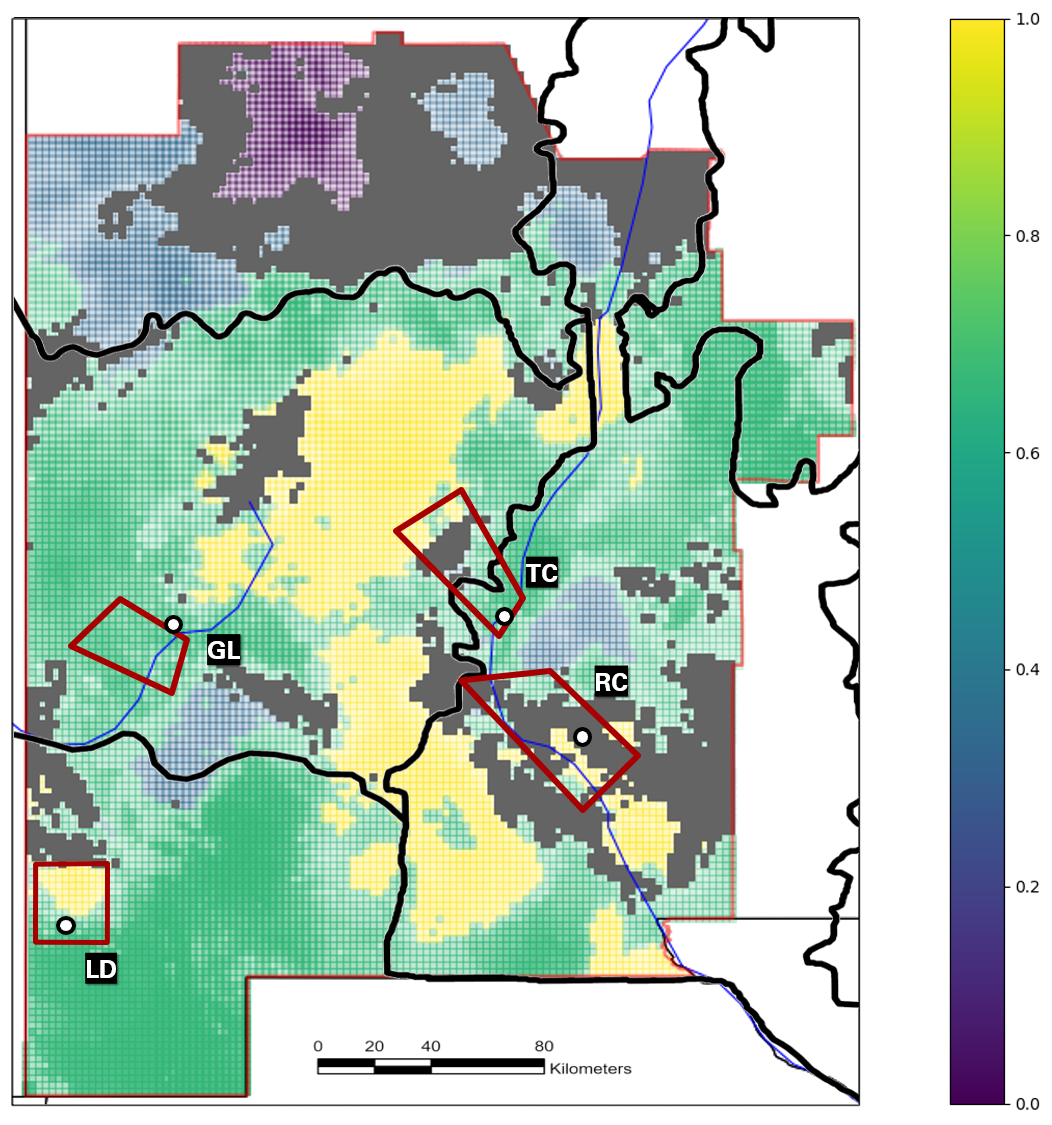
\includegraphics[width=.75\textwidth]{templates/images/Figure-Masked_Average_Gradient_Map-Prospect_Zones.png}
\caption[Structural uncertainty map with prospective areas]
{Combined-model prediction map with uncertainty masking as described for Figure \ref{fig:avg_gradient_masked_map}. Dark red quadrangles and labels identify prospective locations discussed in the text. Bold black lines depict the boundaries between the main physiographic regions in the study area. White markers plot KGAs related to the prospects with most-likely resource temperatures > 60 $^\circ$C.}
\label{fig:structural_uncertainty_prospects}
\end{figure}

\begin{figure}
\centering
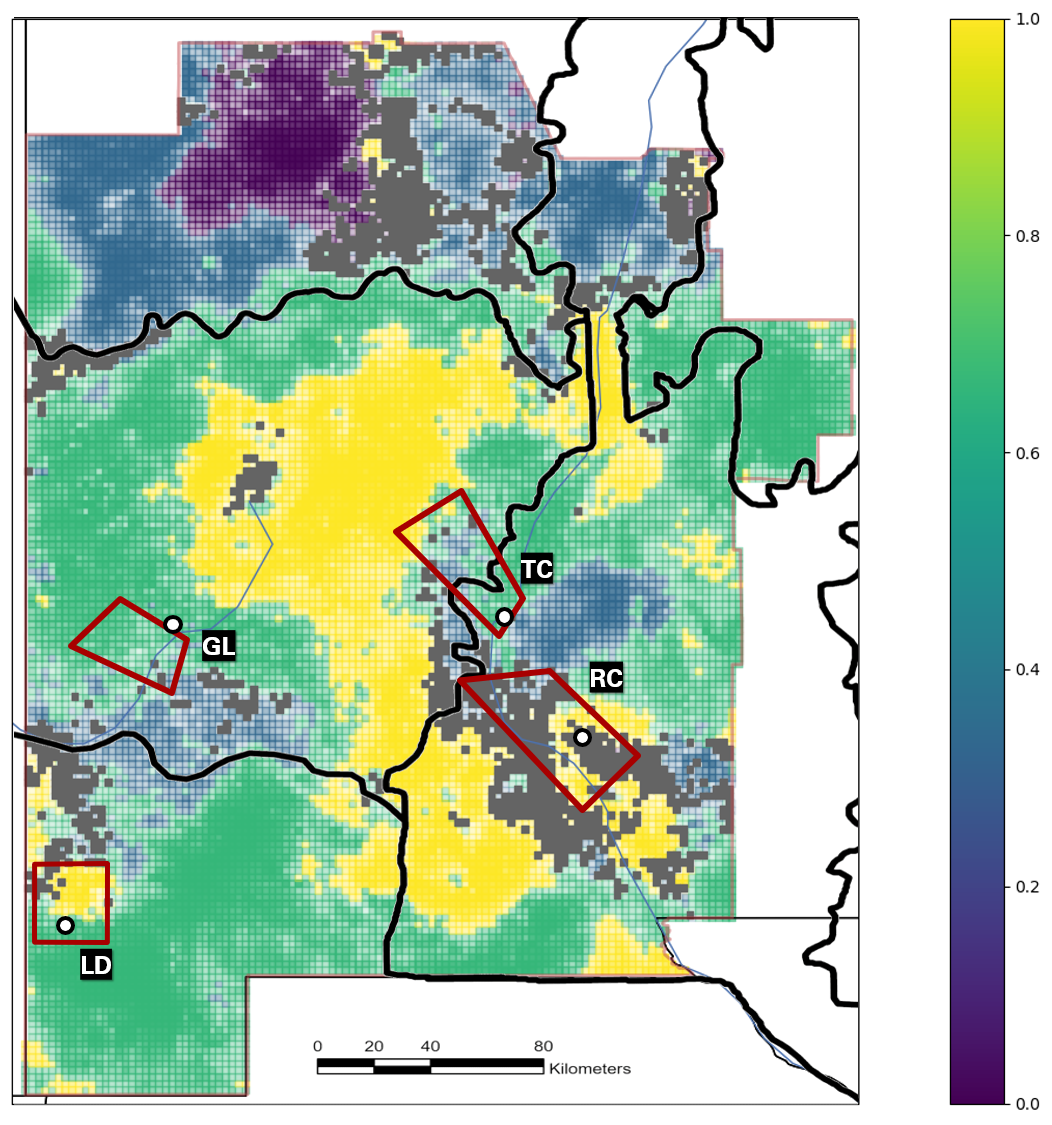
\includegraphics[width=.75\textwidth]{templates/images/Figure-BNN_All_Gradient_Map_Masked_Prospect_Zones.png}
\caption[Parameter uncertainty map with prospective areas]
{BNN ensemble-averaged prediction map with parameter-uncertainty based masking, as described for Figure \ref{fig:bnn_masked_pred_map}. Dark red quadrangles and labels identify prospective locations discussed in the text. Bold black lines depict the boundaries between the main physiographic regions in the study area. White markers plot KGAs related to the prospects with most-likely resource temperatures > 60 $^\circ$C.}
\label{fig:param_uncertainty_prospects}
\end{figure}

Figure \ref{fig:param_uncertainty_prospects} illustrates parameter uncertainty based on repeated runs of the BNN model. Gradient predictions for LD, GL, and TC all share moderate to high certainty. However, low parameter certainty is observed throughout the RC area. This uncertainty may at least partly account for the diversity of geothermal gradient class assignments within the RC quadrangle by the ANN model (Figure \ref{fig:ml_models_prospects}D). If RC was a target prospect, using predictions from the neural network alone to guide next steps would not be advised given the level of uncertainty. Explorationists would do well to choose a different, more certain model, particularly if no additional data are available for training the neural network further.

\begin{figure}
\centering
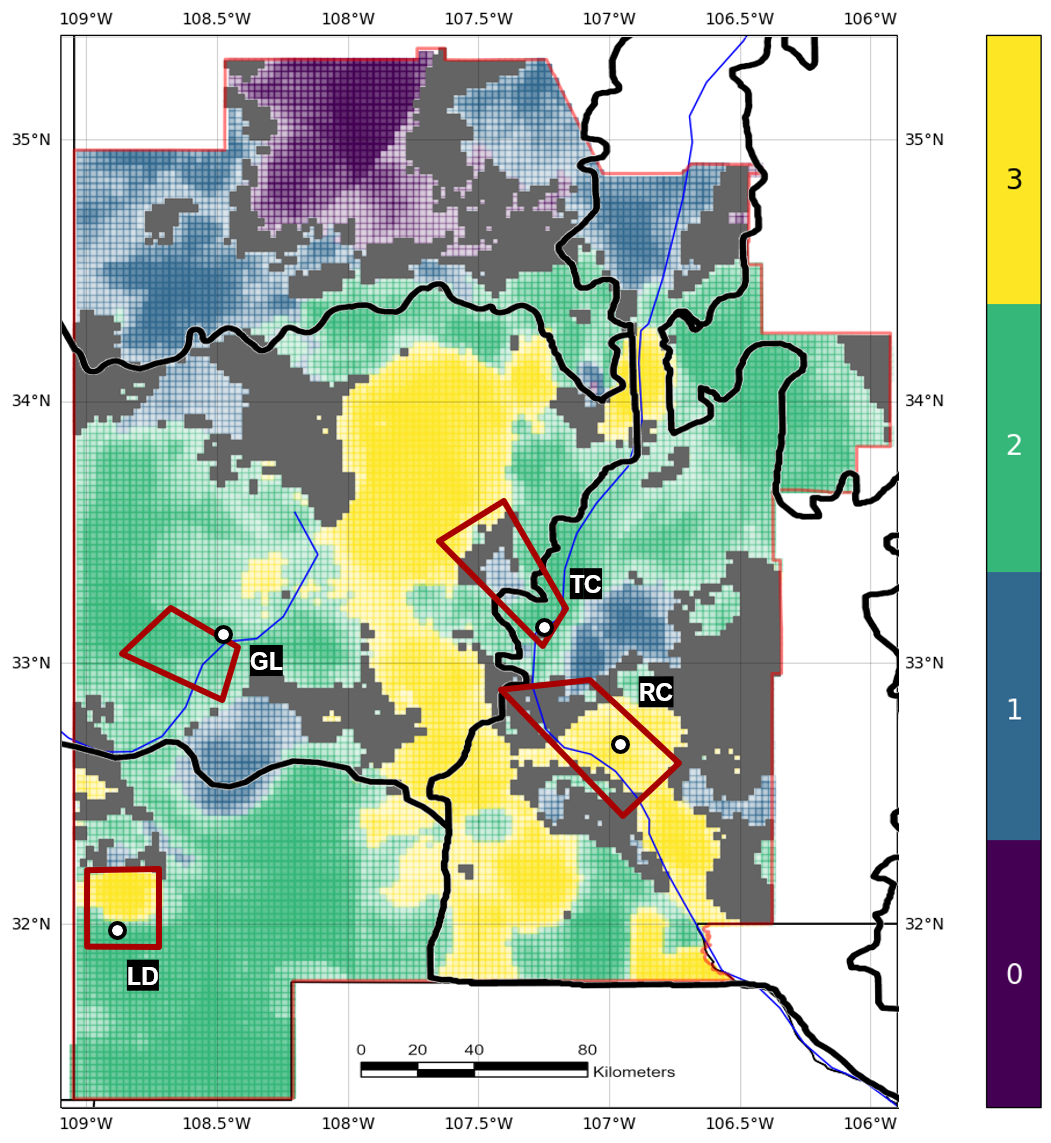
\includegraphics[width=.75\textwidth]{templates/images/Figure-MU_Masked_Average_Gradient_Map_Prospect_Zones.png}
\caption[Measurement uncertainty map with prospective areas]
{Ensemble-averaged WDS4 XGBoost prediction map with SiGT measurement uncertainty masking as described for Figure \ref{fig:mu_masked_pred_map}. Dark red quadrangles and labels identify prospective locations discussed in the text. Bold black lines depict the boundaries between the main physiographic regions in the study area. White markers plot KGAs related to the prospects with most-likely resource temperatures > 60 $^\circ$C.}
\label{fig:measure_uncertainty_prospects}
\end{figure}

Measurement uncertainty depicted in Figure \ref{fig:measure_uncertainty_prospects} considers Si Geothermometer Temperature (SiGT) in isolation from the rest of the input feature set, noting that SiGT dominates in feature importance for the XGBoost model (see Section \ref{ch5:xgb_feature_selection}). The level of measurement certainty for all four prospective areas is striking. A strip of low certainty appears at the gradient class boundary at TC, and likewise to the NW for Rincon. However, these results indicate no strong need to supplement or replace the SiGT data for the prospect areas, as might be the case for other locations within the AOI.

\noindent
In summary, the uncertainty analysis shows:
\begin{itemize}[itemsep=2pt]
    \item All models agree LD has the best high-grade gradient potential, while GL and TC are less prospective. The models are collectively inconclusive on RC.
    \item Neural-network parameter uncertainty makes it an unreliable model for assessing the RC area.
    \item SiGT measurements are relatively certain for the prospect areas. Additional expenditures for SiGT data may not be necessary.
\end{itemize}
Treating this analysis as part of a hypothetical exploration program, the overall heat-element favorability and low uncertainty would make LD a good prospect to progress to the well-planning stage. High uncertainty at RC would need to be addressed through additional pre-screening efforts before committing the resources and capital to drilling there.

\subsection{Southwestern New Mexico PCA}\label{ch5:case_nm_pca}

In a more recent study, \citet{pepin_new_2019} applied unsupervised PCA with $K$-means clustering to assess the geothermal potential of the Southwestern NM study area. \citeauthor{pepin_new_2019} noted the physiographic provinces in NM exert strong controls on the presence and type of USGS-identified KGRAs observed across the state. The cluster analysis identified two high-potential zones with different characteristics. The first defines a predominantly high-temperature hydrothermal zone stretching east-west from LD to the eastern AOI boundary and up along the Rio Grande to just above RC \citep[][Figure 3.5A]{pepin_new_2019}. A second high-potential region surrounds the narrow zone where CP, MDVF, RGR, and GP provinces all converge \citep[][Figure 3.5C]{pepin_new_2019}, although this second group largely comprises systems with low-temperature hot springs. 

The supervised-learning results presented in Figures \ref{fig:ml_models_prospects} and \ref{fig:structural_uncertainty_prospects} clearly display a correlation between high-grade geothermal gradient and physiographic province, but the relationship differs from that described by \citet{pepin_new_2019}. Models consistently predict high-grade gradients in the southern RGR and eastern MDVF provinces, with an additional ``hot spot'' where the RGR narrows to the north. This pattern repeats for all four machine learning models, and is present, albeit less obvious, in the geothermal-gradient feature map from \citet{bielicki_hydrogeolgic_2015} (see Figure \ref{fig:pfa_prospects}). \citet{pepin_new_2019} places the MDVF province in a low-potential cluster, driven in part by risk elements not considered here like structure/permeability. Nevertheless, the PCA model shows relatively strong overlap between clusters \citep[][Figure 3.4]{pepin_new_2019}, suggesting additional data engineering or alternative dimensionality-reduction methods could be of value before fully-discounting the prospectivity of the MDVF province.

Cluster analysis shows great promise, particularly in identifying how the influence of different features changes across a study area. \citet{pepin_new_2019}, \citet{smith_characterizing_2021}, and \citet{vesselinov_discovering_2020} all illustrate this point with significantly different dominant predictors for clusters correlated to individual physiographic provinces. Similar variance in feature importances was observed in the Shapley analysis by class (Figure \ref{fig:xgb_shap_global}); e.g., Si Geothermometer Temperatures top the importance list for class 0 and 1, but come in 2nd to Volcanic Dikes for class 3, and 4th from last in importance for class 2.

Perhaps more interesting is the relationship between high-grade geothermal gradients and complex physiographic province \textit{junctions} (i.e., physical geography interfaces) as seen in Figure \ref{fig:ml_models_prospects}. Specifically, the two boundary zones between 3 or 4 provinces within the AOI both have consistent high-grade geothermal gradient classifications. These zones also correspond with the two prospective clusters in the PCA analysis \citep{pepin_new_2019}. Whether greater geothermal potential at complex province junctions is unique to this study area or more broadly applicable requires further research.

\section{Recap}\label{ch5:recap}

This chapter presented the results from applying the four supervised machine-learning models described in Chapter \ref{ch3:expl_ml_prep} to the curated data (Appendix \ref{app:A_data_layers}) for the Southwestern NM study area. Uncertainties associated with the choice of models, the model parameters, and data measurements were also examined in the context of next-steps decisions for an explorationist. The chapter concluded with a comparison with other geothermal prospectivity studies for the region.

\noindent
Key insights from the work include:
\begin{enumerate}
    \item Logistic regression models are simple and easy to tune, however other model techniques have much stronger predictive performance.
    \item Decision trees are highly-explainable and directly identify feature importances. A notable downside is results can vary based on random structural variations during construction.
    \item XGBoost models demonstrate very strong predictive performance and support best-in-class Shapley feature attribution analysis. However, XGBoost model tuning can be complex and time-consuming.
    \item The highest degree of model complexity comes from neural network architectures, which show great performance if sufficient training data is available to constrain the enormous number of model parameters.
    \item Structural uncertainty analysis highlights areas where models collectively differ or agree on predictions. This is useful for rationalizing model selection and identifying spatial areas that require further study before taking costly actions.
    \item Parameter uncertainties indicate the ``known unknowns'' for a model, i.e., locations where model predictions are poorly constrained. Corrective actions include training on more data or relying on a different model technique.
    \item Measurement uncertainties characterize the impact of data reliability on model predictions. If high uncertainty exists in an area of interest, additional data acquisition may be needed, especially from sources with lower standard errors. 
    \item The value of this approach to exploration risk mitigation is demonstrated for  prospective areas identified in the Southwestern NM PFA study. High favorability, low uncertainty prospects (e.g., Lightning Dock) could progress to a well-planning stage, but areas with mixed favorability and/or high uncertainty (e.g., Rincon) would require additional pre-screening first.
    \item A correlation between physiographic provinces and geothermal favorability established in other studies is also observed in the Southwestern NM study area. In addition, high-grade geothermal gradients (positive heat risk-element values) align with complex convergence zones between 3 or more physiographic provinces.
\end{enumerate}
